\documentclass[../main.tex]{subfiles}

\begin{document}
\chapter{Experimental evaluation}\label{exp}
In the preceding chapters, we have built up the theory around games and the methods to discover their solution.
Then, modifications of these algorithms, which do not necessarily require linear programming formalism to determine the approximate results, were proposed.
This chapter consists of comparing different multi-armed bandit algorithms within these modified methods on two distinct models.

Firstly, we study the performance and the convergence of distinct bandits, used in the bandit iteration algorithm proposed in \refsec{new:bandititeration}, to the optimal value found by the value iteration method on the model of fully observable stochastic games.
We will mostly focus on comparing the observable and standard variants as well as the two different accumulation steps \refsec{new:bandititeration:steps}, $\lint$ and $\sqrtt$.

Secondly, we compare convergence of the B-HSVI \refsec{new:bhsvi} algorithm also using multi-armed bandits with the standard HSVI \refsec{standard:osposg} which uses mathematical programming.
In this case, we focus on partially observable stochastic games and specifically on the OS-POSGs subset, even though this algorithm can solve perfect information stochastic games, too.

\section{Technical details}\label{exp:tech}
The experiments were carried out through the \textit{Metacentrum} platform acknowledged at the preface of the thesis, specifically on the \textit{halmir} cluster \cite{halmir}.
For a single run of an algorithm was used a single AMD EPYC 7543 core with $2.8$GHz base frequency and $16$GB of RAM.
The algorithms were implemented in a single-threaded program in the programming language Julia, version (1.7.0) \cite{julia}.
For the linear programs, the \textit{Coin-or linear programming} \cite{clp} and \textit{IBM CPLEX v. 20.1} optimization frameworks were used.
The implementation details for solution methods of both evaluated algorithms are listed in \refapx{apx:impl}.

\section{SGs and bandit iteration}\label{exp:sg}
In \refsec{bg:sg} a formal model of a stochastic game was introduced and an algorithm provided to solve any instance declared in this formalism in \refsec{standard:sg}.
It was modified to create \textit{bandit iteration} algorithm in \refsec{new:bandititeration}.
For comparison purposes of this thesis, we used two specific game types, each consisting of multiple different instances.
Before proceeding with the experimental testing of the algorithm, we define the two types of games.
The games are quite simple and the particular used instances are small so many results of the experiments can be at least partly verified by intuition.

\subsection{Game types}\label{exp:sg:games}
In both games, there are two players placed in a maze-like environment.
The players simultaneously choose actions and move through the maze or carry out extra manoeuvres and while player 1 tries to defeat player 2 as quickly as possible, player 2 tries to stay alive as long as he can.

Both players can observe positions and formerly chosen actions of the adversary, the only thing unknown to them is the action selected in the current round.
Because these are types of \textit{stochastic} games, every selected action can have multiple outcomes with different probabilities.
For example, if a player decides to go forward, he can end up somewhere else than before him with some non-zero probability.
However, these outcomes and probabilities depend on the particular instance of a game type and are not essential for the understanding of the game.
Henceforth, for the sake of a simpler description, we will assume that each action has only a single outcome, i.e. the player always does what was intended.

For both types, it is possible, that the game will take infinitely long.
As any player can perfectly observe its adversary, it just depends on the specific instance.
We try to avoid this situation by posing a restriction that there always exists some path between both players.

\subsubsection{Chase}\label{exp:sg:games:chase}
The game we call \textit{Chase} is the simpler of the two types.
It takes place in a randomly generated directed graph $g = (V, E)$ with loops allowed, where $V$ is a set of vertices of size $n$ and $E$ is a set of directed edges.
The edges connect the $n$ vertices in such a way, that there always exists a path between any two different nodes in the graph.

Player 1, i.e. \textit{chaser}, and player 2, i.e. \textit{runner}, are then located in random vertices $v_1$, $v_2$ in $g$.
Actions available to both players in a vertex $v$ correspond exactly to outgoing edges from the vertex $v$.
An action identified with edge $\left(v,v^{\prime}\right)$ means that a player can move from vertex $v$ to the adjacent vertex $v^{\prime}$.

Players use these actions to move through the graph $g$ and the goal for player 1 is to \textit{catch} player 2, which happens when they end up in the same vertex.
When this phenomenon occurs, they are both moved to a special absorbing state $n+1$, which is not shown on the visualizations \reffig{exp:sg:games:chase:examples}, and the game ends.
The only exception to this rule, when both can be present in the same vertex and the game does not end, is the initial round $0$, because both can be placed in the same vertex $v_1 = v_2$.
In this case, the game continues and ends only if they immediately go to a same vertex again.

To motivate the chaser to catch the runner the rewards are defined as follows.
Every chaser's action, which does not lead to victory, is penalized with $-1$.
When the runner is caught, the chaser receives a reward $+10$.
The chaser is trying to maximize the total received reward over all rounds and thus trying to win soon.
On the contrary, from the definition of a two-player zero-sum game, the runner is trying to minimize this quantity and avoid being caught for as long as possible.

\begin{figure}[ht]
    \centering
    \begin{subfigure}[b]{0.3\textwidth}
        \centering
        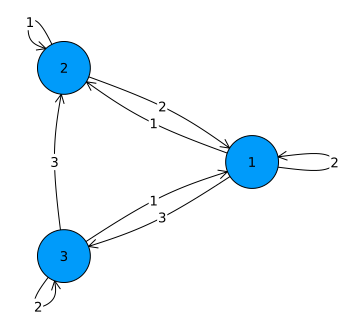
\includegraphics[width=\textwidth]{games/chase_3.png}
        \caption{\textbf{Chase3} with $n = 3$}
        \label{exp:sg:games:chase:examples:3}
    \end{subfigure}
    \hfill
    \begin{subfigure}[b]{0.3\textwidth}
        \centering
        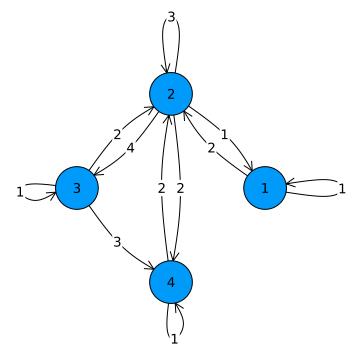
\includegraphics[width=\textwidth]{games/chase_4.png}
        \caption{\textbf{Chase4} with $n = 4$}
        \label{exp:sg:games:chase:examples:4}
    \end{subfigure}
    \hfill
    \begin{subfigure}[b]{0.3\textwidth}
        \centering
        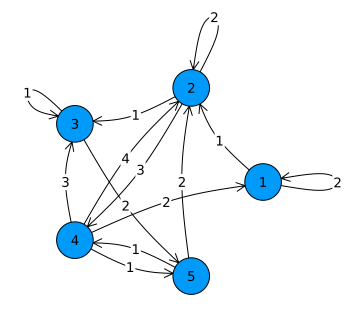
\includegraphics[width=\textwidth]{games/chase_5.png}
        \caption{\textbf{Chase5} with $n = 5$}
        \label{exp:sg:games:chase:examples:5}
    \end{subfigure}
    \caption[Example \textbf{Chase} instances]{Illustration of graphs representing the environment of the \textbf{Chase} stochastic game for different number of vertices. The detailed description of \textbf{Chase} is in \refsec{exp:sg:games:chase}. Numbers in vertices of the graphs represent identifiers of the states of the game and the integers near the edges are labels for corresponding actions.}
    \label{exp:sg:games:chase:examples}
\end{figure}

\subsubsection{Tag}\label{exp:sg:games:tag}
As opposed to \textit{Chase}, \textit{Tag} is closer to more conventional games.
Player 1 is called tagger, while player 2 is named evader.
Players are randomly placed into a square $n \times n$ board with some obstacles, which do not permit the player to pass through them.
The only restriction to the placement of obstacles is, as mentioned before, that there must exist a path between the two players so that solving the game even makes sense.

Both players have actions to move to adjacent squares if there is no obstacle present on the target square.
In addition, the tagger can shoot a laser beam either vertically or horizontally in every state.
In this case, player 2 stays on the square he was before shooting and the beam hits all squares in the chosen direction until an obstacle or end of the map is hit.

The goal of the tagger is not to get on the same square as the evader, as it was in \textit{Chase}, but to hit the evader with the laser beam.
Again, he tries to succeed as fast as possible and player 2 tries to avoid getting hit for the longest.
Rewards for moving and completing the objective remain the same as in \textit{Chase}.
However, to discourage the tagger from shooting unnecessarily, blasting a laser beam without hitting the target results in a bigger penalization by reward $-10$.
As well as in \textit{Chase}, player 1 tries to maximize the overall accumulated reward and player 2 tries to minimize it.

\begin{figure}[ht]
    \centering
    \begin{subfigure}[b]{0.3\textwidth}
        \centering
        \begin{tikzpicture}
            \foreach \x in {0,1}{\foreach \y in {0,1}\node[box] at (\x,\y){};}
            \node[box] at (0, 1) {1};
            \node[box] at (1, 1) {2};

            \node[box,fill=black] at (0, 0) {};
            \node[box] at (1, 0) {3};
        \end{tikzpicture}
        \caption{\textit{Tag} $2 \times 2$}
        \label{exp:sg:games:tag:example:2}
    \end{subfigure}
    \hfill
    \begin{subfigure}[b]{0.3\textwidth}
        \centering
        \begin{tikzpicture}
            \foreach \x in {0,1,2}{\foreach \y in {0,1,2}\node[box] at (\x,\y){};}
            \node[box] at (0, 2) {1};
            \node[box, fill=black] at (1, 2) {};
            \node[box] at (2, 2) {5};

            \node[box] at (0, 1) {2};
            \node[box, fill=black] at (1, 1) {};
            \node[box] at (2, 1) {6};

            \node[box] at (0, 0) {3};
            \node[box] at (1, 0) {4};
            \node[box] at (2, 0) {7};
        \end{tikzpicture}
        \caption{\tagname{3}{01} $3 \times 3$}
        \label{exp:sg:games:tag:examples:31}
    \end{subfigure}
    \hfill
    \begin{subfigure}[b]{0.3\textwidth}
        \centering
        \begin{tikzpicture}
            \foreach \x in {0,1,2}{\foreach \y in {0,1,2}\node[box] at (\x,\y){};}
            \node[box] at (0, 2) {1};
            \node[box] at (1, 2) {3};
            \node[box, fill=black] at (2, 2) {};

            \node[box] at (0, 1) {2};
            \node[box] at (1, 1) {4};
            \node[box] at (2, 1) {6};

            \node[box, fill=black] at (0, 0) {};
            \node[box] at (1, 0) {5};
            \node[box] at (2, 0) {7};
        \end{tikzpicture}
        \caption{\tagname{3}{02} $3 \times 3$}
        \label{exp:sg:games:tag:examples:32}
    \end{subfigure}
    \caption[Example \textbf{Tag} instances]{Illustration of the maze, where the tagger tries to shoot the evader in the \textbf{Tag} game described fully in \refsec{exp:sg:games:tag}. Both players cannot step on the black fields. The states available for them are labelled with unique integer identifiers used in later comparisons.}
    \label{exp:sg:games:tag:examples}
\end{figure}

When the evader is hit, the game ends and both players are again moved into an absorbing terminal state, which is again not shown in the pictures \reffig{exp:sg:games:tag:examples}.

\subsection{Environment and parameters}\label{exp:sg:env}
The performance of an algorithm depends not only on the algorithm itself but also on its parameters and the settings of the environment where the algorithm is put.
Here, the most important parameters are the bandit ones as they drive the search.
These details are briefly described in this section.

\subsubsection{Reference}\label{exp:sg:env:ref}
To argument about convergence of a given bandit algorithm used inside the bandit iteration framework \refalg{new:bandititeration:alg} some referential value is needed.
The values returned by the algorithm are then supposed to get as close as possible to this reference value.
Ideally, they should be equal.

The best possible reference value is the optimal value, but this value is unknown.
Thus, the value returned by the value iteration algorithm, after it stopped with some precision parameter $\Delta$.
From the definition of value iteration \refalg{standard:sg:valueiter:algorithm:alg}, the returned value function $V_{\text{iter}}(s)$ is a good approximation of the optimal $V^*(s)$ in every state $s \in S$.
For the purpose of the following comparisons, we pose $V^* = V_{\text{iter}}$ and the values returned from the bandit iteration algorithm are compared to this value.
The precision parameter was set to $\Delta = 1 \times 10^{-6}$.

For comparing the results of the bandit algorithm with different bandits, we use quantities $V(s)$ based on this formula
\begin{equation}\label{exp:sg:env:ref:diff}
    V(s) = V_{\text{bandit}}(s) - V^* \qquad \forall s \in S
\end{equation}
When $V(s) = 0 \quad \forall s \in S$, we say that the bandit iteration has converged.

\subsubsection{Means of evaluation}\label{exp:sg:env:eval}
In stochastic games, there is defined a starting state, where both players begin their plays.
Solving the game then means finding value of the game in this particular starting state.
However, in our experiments, we always perform the learning backup for every state $s \in S$ and thus we end with value of the game for every state.
To acquire the value of the game for the starting point, it only needs to be picked from the value function $V_{\text{bandit}}$.
This way is convenient for comparison of the bandit algorithms and how they behave in different types of states.

\subsubsection{Setting}\label{exp:sg:env:runs}
Experiments were run on all three \textit{Chase} instances \reffig{exp:sg:games:chase:examples}, for one \textit{Tag} instance with dimensions $2 \times 2$ \reffig{exp:sg:games:tag:example:2} and for $7$ instance of \textit{Tag} with dimensions $3 \times 3$.
Two of those latter instances are displayed in \reffig{exp:sg:games:tag:examples:31}, respectively \reffig{exp:sg:games:tag:examples:32}.

The versions of multi-armed bandits from \refsec{new:bandit} were used in the bandit iteration algorithm for evaluation, which are those with shuffled greedy action selection, the observable variants and the numerically stable Exp3.
Every bandit was tried inside the bandit iteration for $10^5$ iterations $10$ times for each instance for both steps, $\lint$ and $\sqrtt$ \refdef{new:bandititeration:steps}, with different seeds for each single run.

The runtime of these bandit iteration runs for different instances of \textit{Tag} and \textit{Chase} is analysed in \refapx{apx:time}.

\subsubsection{Parameters}\label{exp:sg:env:parameters}
The parameters were fixed to those used standardly with each respective bandit.
Both the observable and non-observable variants were parametrized with the same value, so the comparison is more accurate.
The individual chosen parameters for all non-observable bandits are listed in table \reftab{exp:sg:env:params:params}.
\begin{table}
    \begin{tabular}{l || c | c | c | c | c}
        bandit & Best of N & $\epsilon$-greedy & Successive elimination & UCB & Exp3 \\
        \hline
        parameter & $N = 100$ & $\epsilon = 0.1$ & \multicolumn{2}{c |}{$\alpha = 20$} & $n = 10^5$
    \end{tabular}
    \caption[Selected parameters for multi-armed bandits for the bandit iteration algorithm]{The best found parameter values for each individual bandit algorithm tested on stochastic games in the bandit iteration framework.}
    \label{exp:sg:env:params:params}
\end{table}

For the Best of N bandit, the N should be much smaller than the intended number of iterations, otherwise it would degrade into simply random selection as the first $N * |A|$ actions are selected uniformly at random.
The chosen number is shown in \reftab{exp:sg:env:params:params}

The value $\epsilon = 0.1$ is used usually for the $\epsilon$-greedy as it provides sufficient exploration while exploiting very frequently.

The exploration parameter $\alpha$ has the same purpose for both Successive elimination and UCB bandits as it represents how fast do the confidence bounds tighten around the average received reward.
A good rule of thumb for selecting this value is the size of an interval, from which the rewards are sampled.
In the case of \textit{Catch}, the interval is $\left[-1, 10\right]$, so the parameter should be $\alpha_{\text{catch}} = 11$, for \textit{Tag} it is $\left[-10, 10\right]$, and thus $\alpha_{\text{tag}} = 20$.
Naturally, the larger one was selected as $\alpha$.

The Exp3 is given the number of iterations $n$ as a single parameter and then the appropriate $\gamma$ and $\eta$ are computed as declared in \refform{new:bandit:instability:params}.

The experiments were conducted for different parameter settings with the above in mind.
The values listed in \reftab{exp:sg:env:params:params} showed the best results.

\subsubsection{Graphs}\label{exp:sg:env:graphs}
Graphs are the most important part of the following examination of the algorithm's behaviour.
To prevent confusion, we briefly describe the properties of the used graphs.

Each graph shows how selected bandits behave in a single state of the examined stochastic game.
Values on the $x$ axis correspond to rounds $t = 1, \dots, T$ of the bandit iteration and due to the large $T = 10^5$, this axis is scaled by the decimal logarithm $\log_{10}$.
The values on the $y$ axis then displays the deviation of the result computed by the bandit iteration and the optimal value found by value iteration for each round.
From these differences $V(t) = V_{\text{bandit}}(t) - V^*$ is computed \textit{mean} $\mu(t)$ and the \textit{standard deviation} $\sigma(t)$.
The graph is thus shown as a line $\mu(t)$ surrounded by an interval $\left[\mu(t) - \sigma(t), \mu(t) + \sigma(t)\right]$ $\forall t = 1, \dots, T$.

The deviation of the optimal value from itself is always $0$ and thus is displayed as a constant function $y = 0$ in black.

Now we have everything ready for the actual comparison of the bandit algorithms and their convergence.

\subsection{Individual bandits}\label{exp:sg:individual}
In this short section, we summarize the analysis of the individual bandit algorithms.
We focus on their performance, comparison of the standard and observable variants and investigation of the effects of the two step functions on the course of convergence.
This summary is based on a detailed analysis located in \refapx{apx:sgexp}.

From the comparisons in \refapx{apx:sgexp}, it clearly follows that the observable variants converge faster and closer to the optimal value than the standard bandits.
We demonstrate this on the example of UCB.
This algorithm does not converge to the optimal value in states where mixed strategies are optimal, because it was designed to find the best single action.
However, the observable UCB is able to leverage the average play of the opponent and correctly find the mixed strategy and converge to the optimal value.

Similarly, the $\sqrtt$ step function is superior to the $\lint$ function, but not as definitely as the observable variants are superior to the standard ones.
The $\sqrtt$ causes much faster convergence to the value, but when the value is close to the optimal value it produces high fluctuations in value.
On the other hand, $\lint$ has a smooth course but at the expense of slow convergence.

From the experiments, the best performing algorithms are UCB, $\epsilon$-greedy with their respective observable variants and the Exp3 adversarial bandit.
These algorithms often find the optimal value with either of the step functions.
In contrast, the Best of $N$ bandit and the Successive elimination do not perform well due to fixating a single best action at some point, which happens with these bandits with no means of recovery.

We proceed with comparison of these selected well-performing multi-armed bandits among themselves to analyse their speed and resistance to changes in value.

\subsection{Bulk comparison}\label{exp:sg:best}
Previously, we showcased how the proposed algorithms behave inside the bandit iteration framework and how they converge to the value found by the value iteration.
Also, we compared the standard single-agent versions with the observable versions meant for games.
Now, we focus on the three most promising multi-armed bandits and compare them together on selected states.
Generally, the bandits which stop even considering some action should be avoided, as this action can later be important in the mixed strategy and just more exploration is necessary.

The comparison is conducted on $4$ states, where are many possible actions and where the optimal strategies are mixed which is confirmed by the value iteration.
These selected bandit algorithms usually have no problem with convergence to an optimum in states with pure strategies, so these are more appropriate to showcase the advantages and disadvantages of each individual bandit.
We separate the set-ups by used step function and the version of the algorithm to prevent confusion and increase readability of the charts.

The first state is $s = \left(3, 3\right)$ of the instance \tagname{3}{01} \reffig{exp:sg:games:tag:examples:31}.
\begin{figure}[ht]
    \begin{subfigure}[t]{0.45\linewidth}
        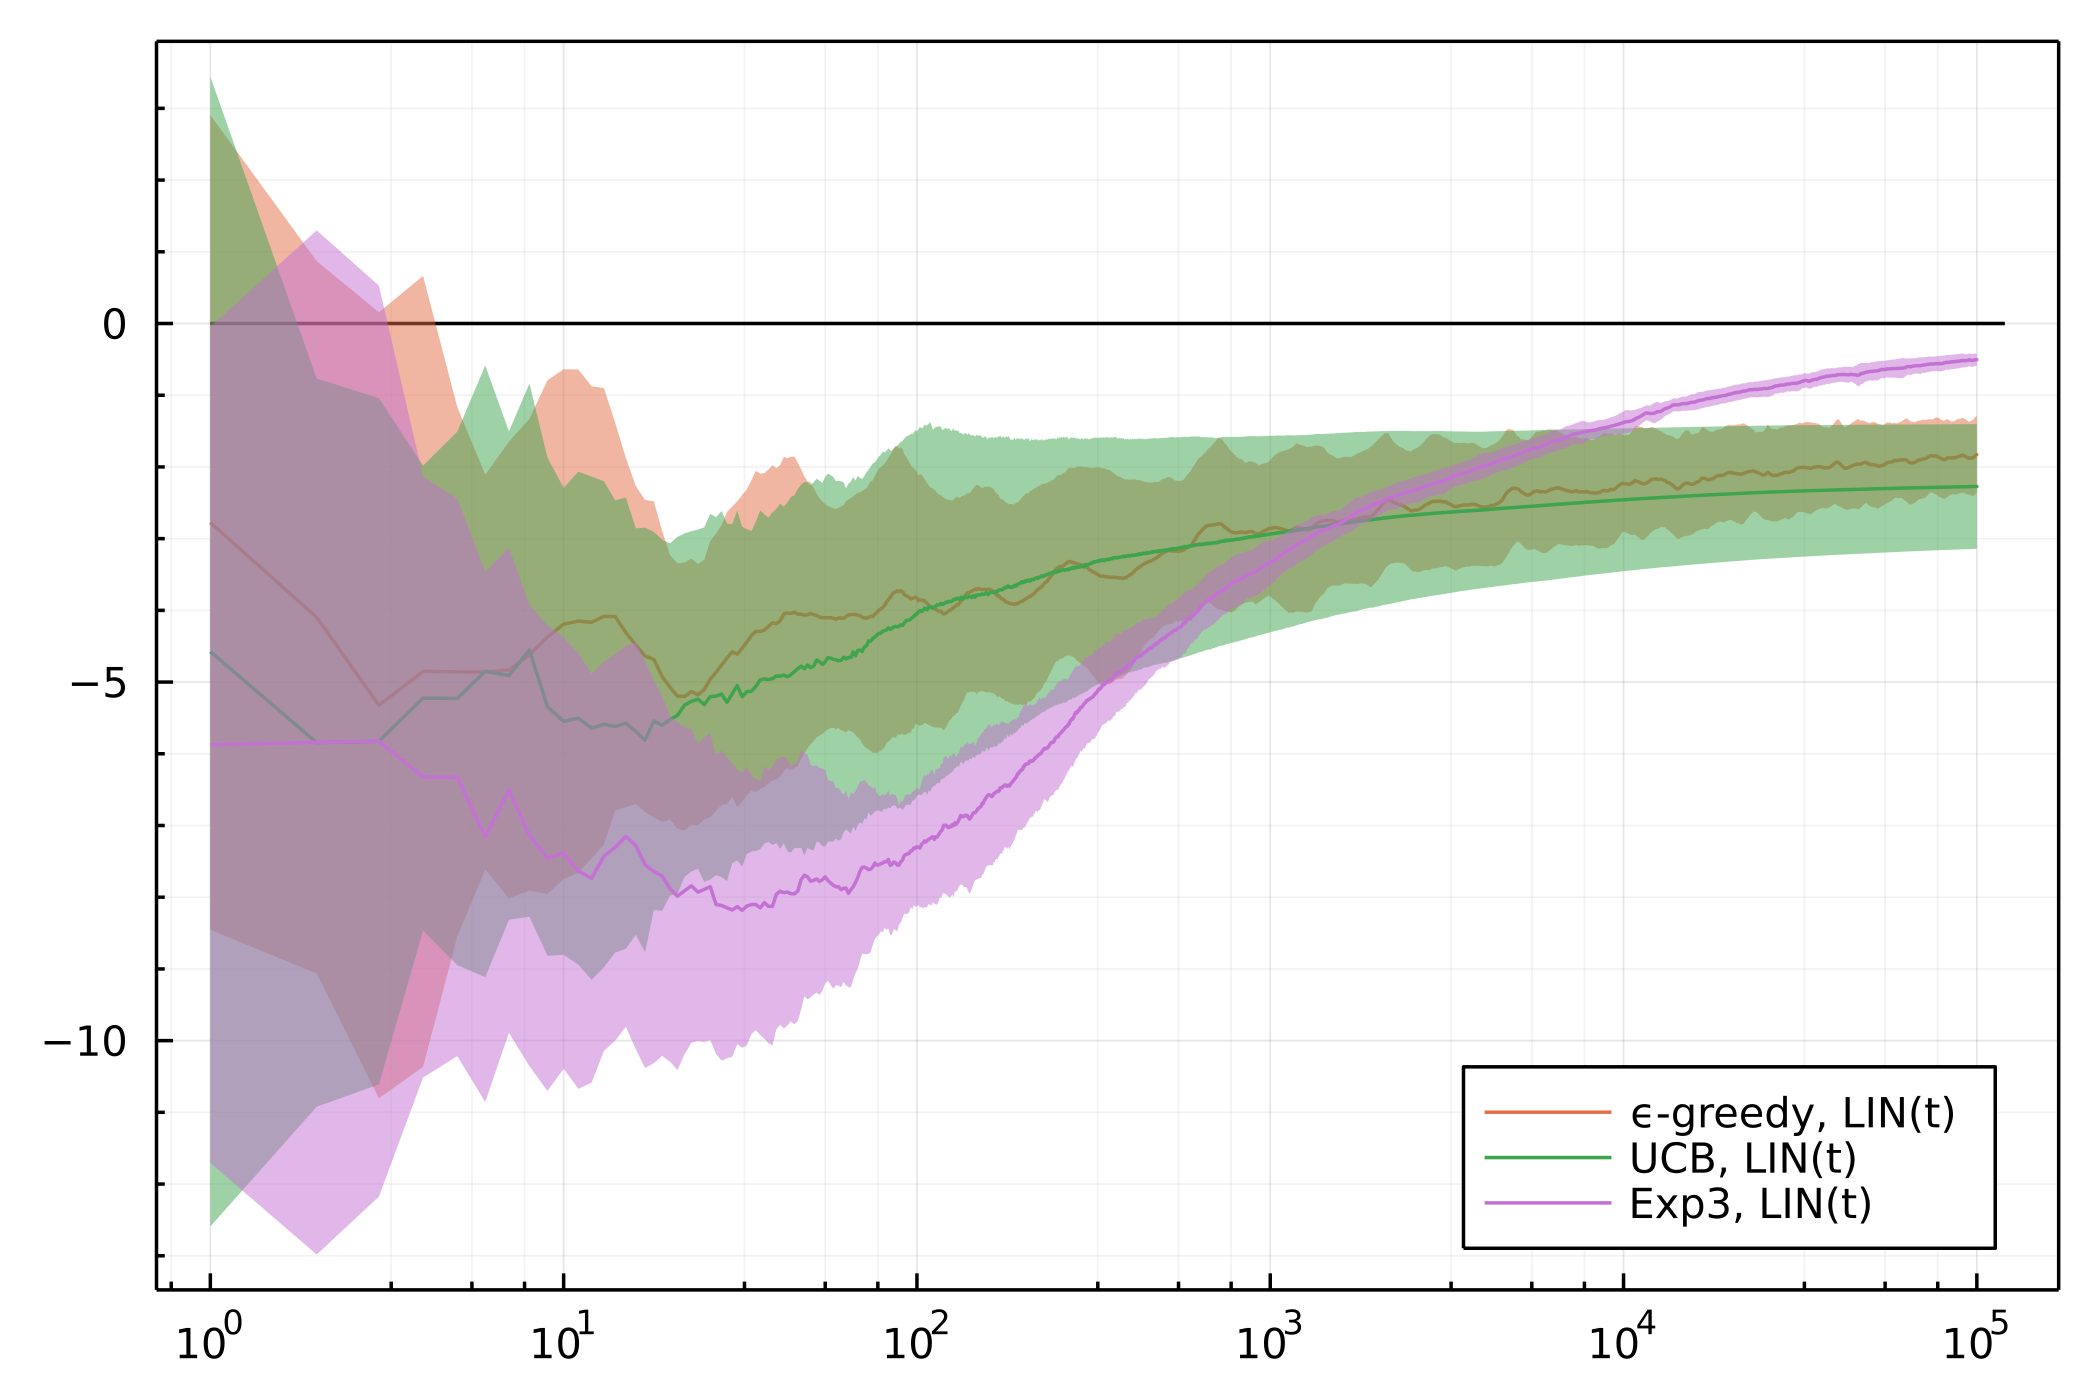
\includegraphics[width=1\textwidth]{sg/best/tag_3_01_EpsilonGreedy_UCB_Exp3_LinT_3_3.png}
        \caption{Standard bandits with $\lint$ step}
        \label{exp:sg:best:301:33:std:lin}
    \end{subfigure}
    \hfill
    \begin{subfigure}[t]{0.45\linewidth}
        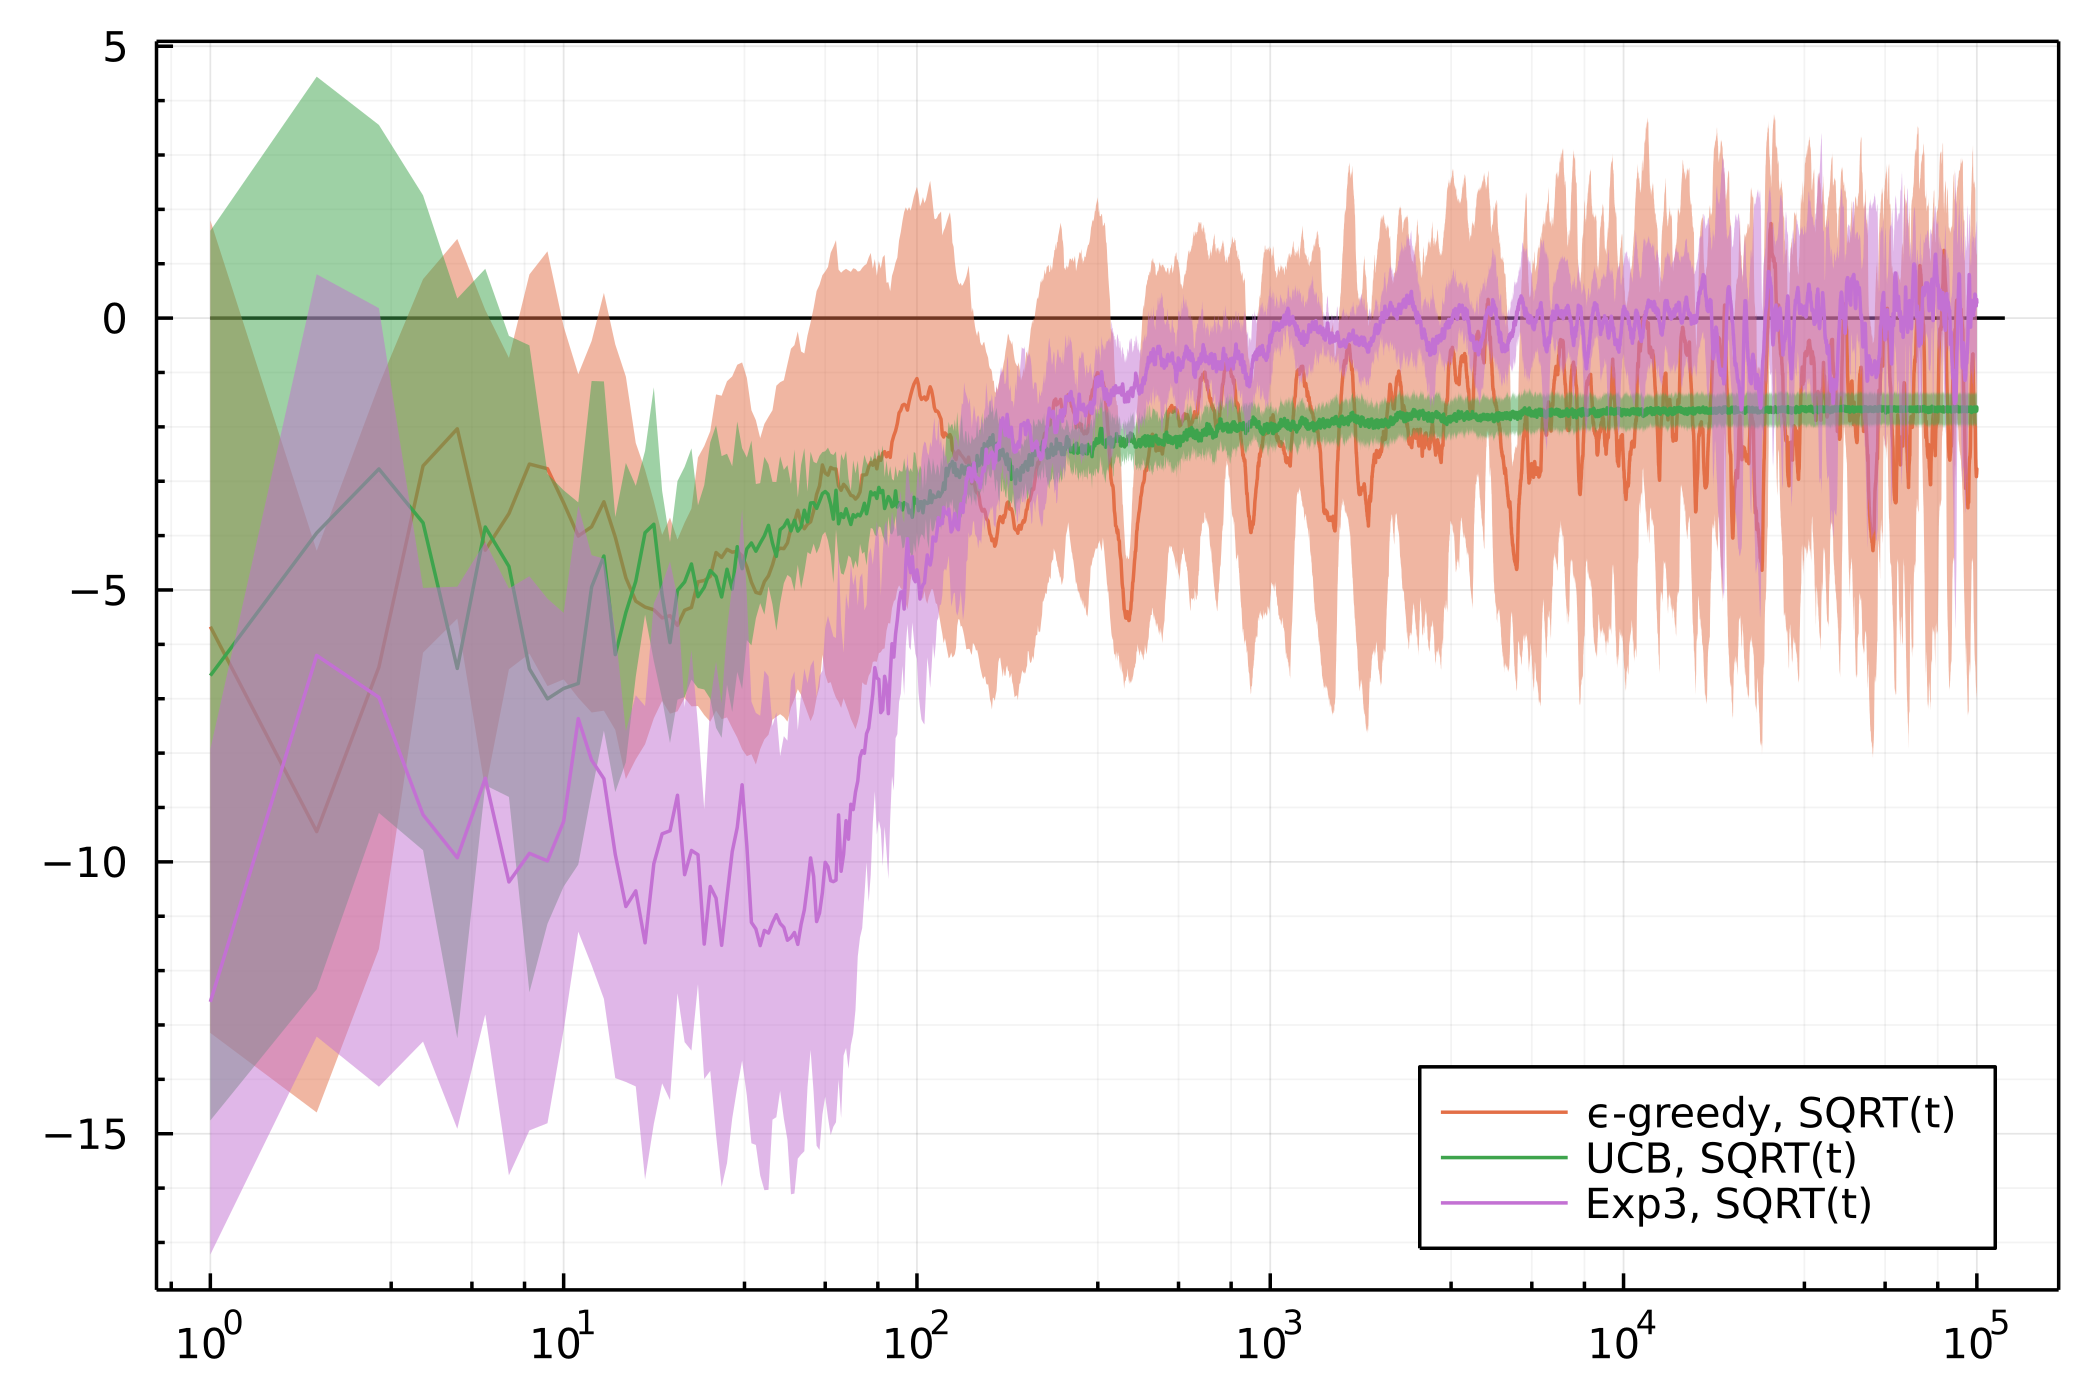
\includegraphics[width=1\textwidth]{sg/best/tag_3_01_EpsilonGreedy_UCB_Exp3_SqrtT_3_3.png}
        \caption{Standard bandits with $\sqrtt$ step}
        \label{exp:sg:best:301:33:std:sqrt}
    \end{subfigure}
    \begin{subfigure}[t]{0.45\linewidth}
        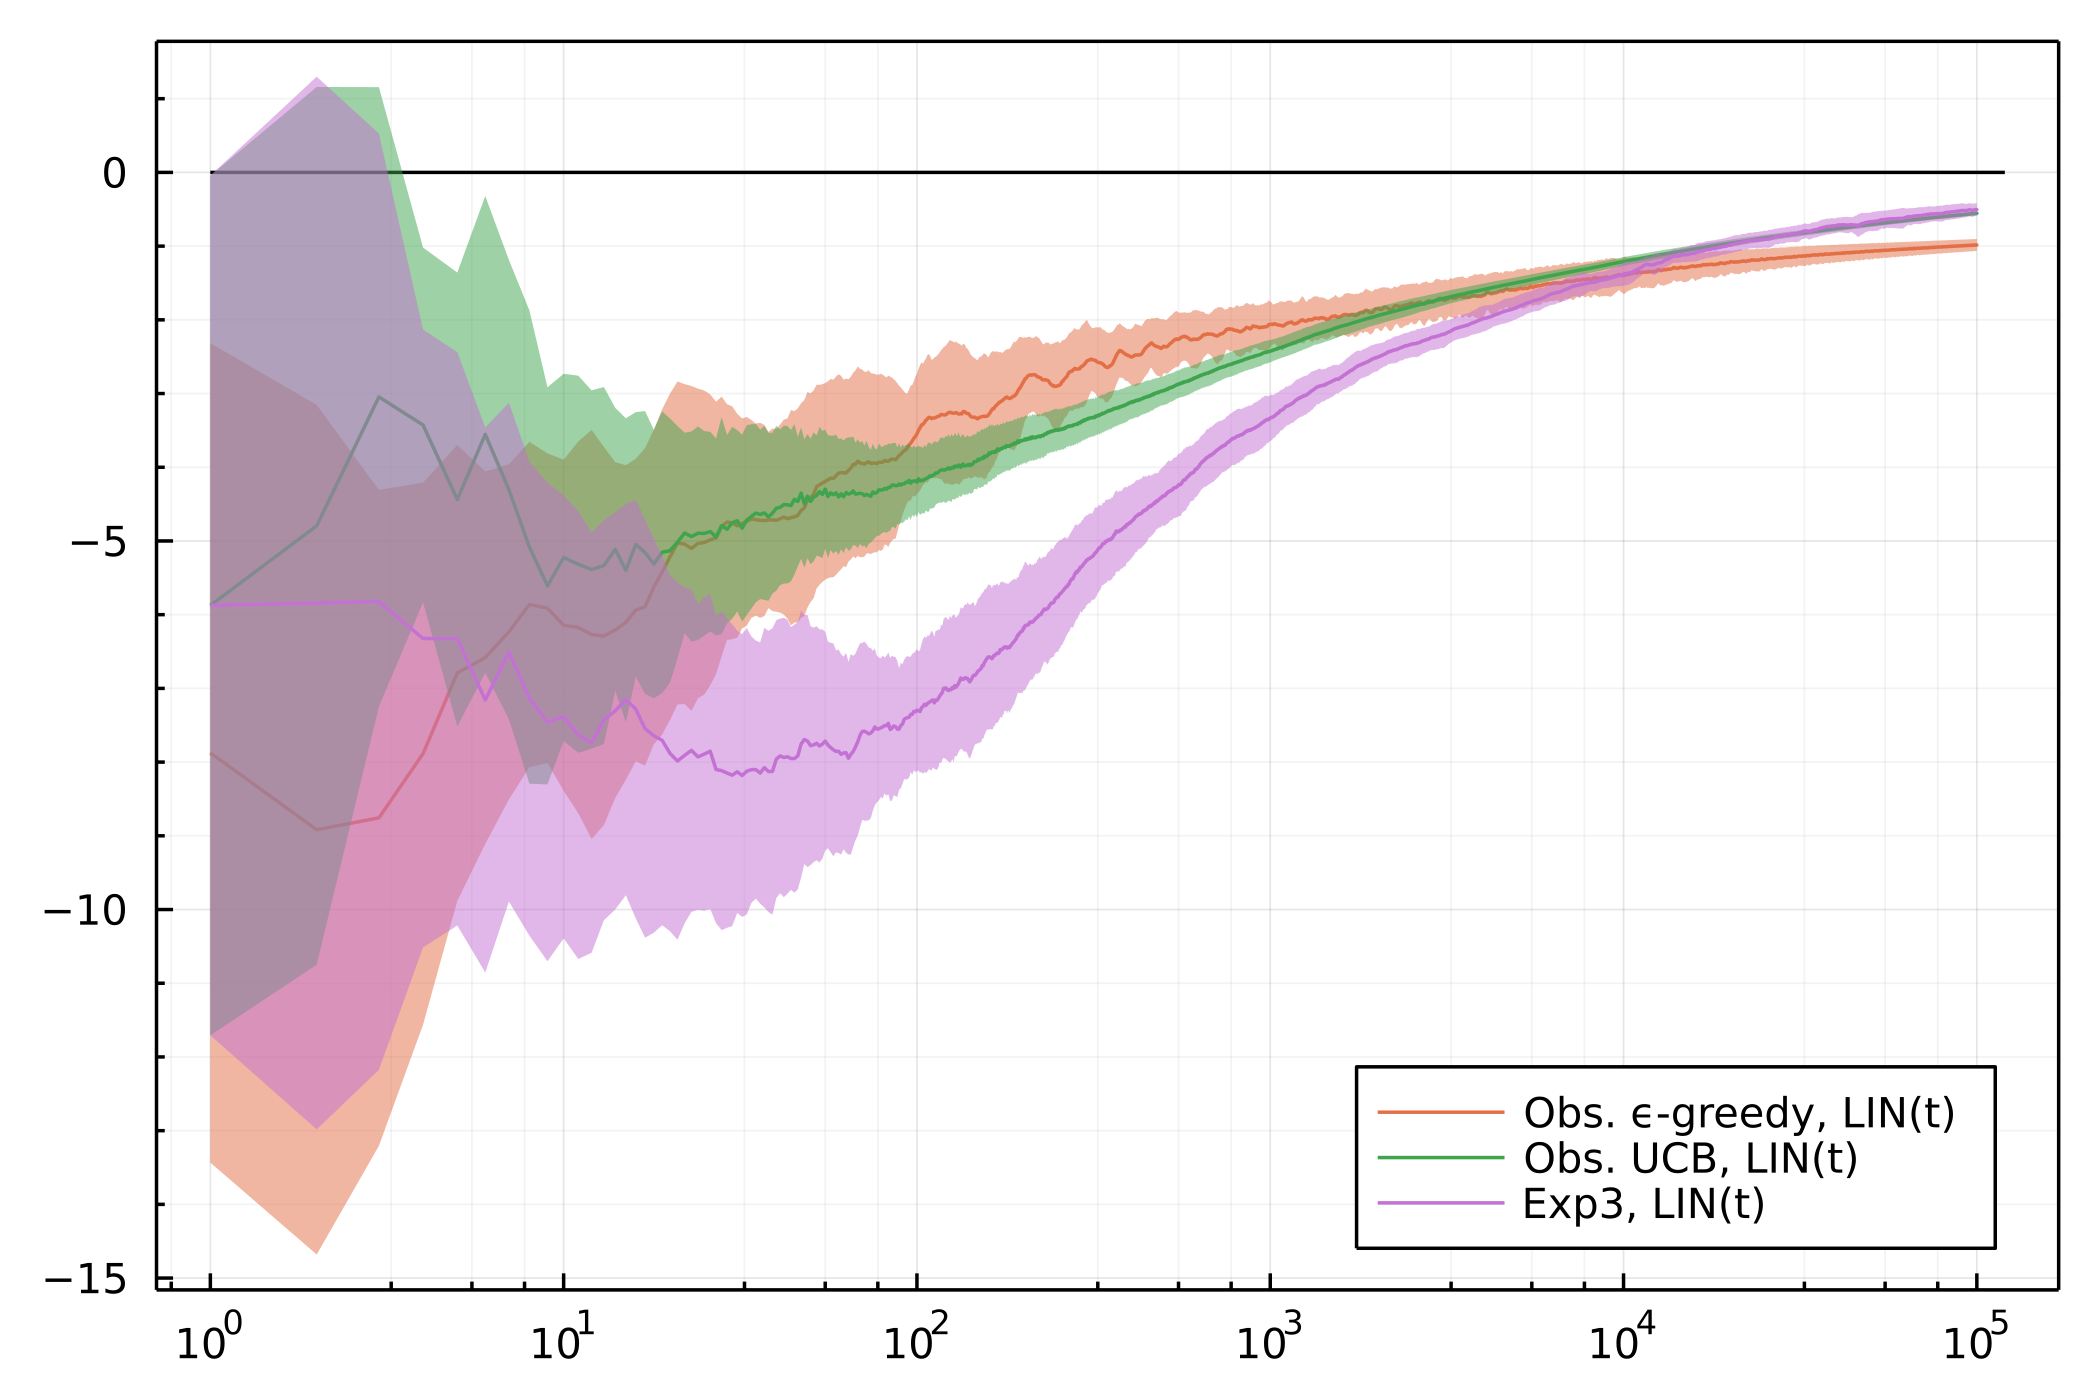
\includegraphics[width=1\textwidth]{sg/best/tag_3_01_ObservableEpsilonGreedy_ObservableUCB_Exp3_LinT_3_3.png}
        \caption{Observable bandits with $\lint$ step}
        \label{exp:sg:best:301:33:obs:lint}
    \end{subfigure}
    \hfill
    \begin{subfigure}[t]{0.45\linewidth}
        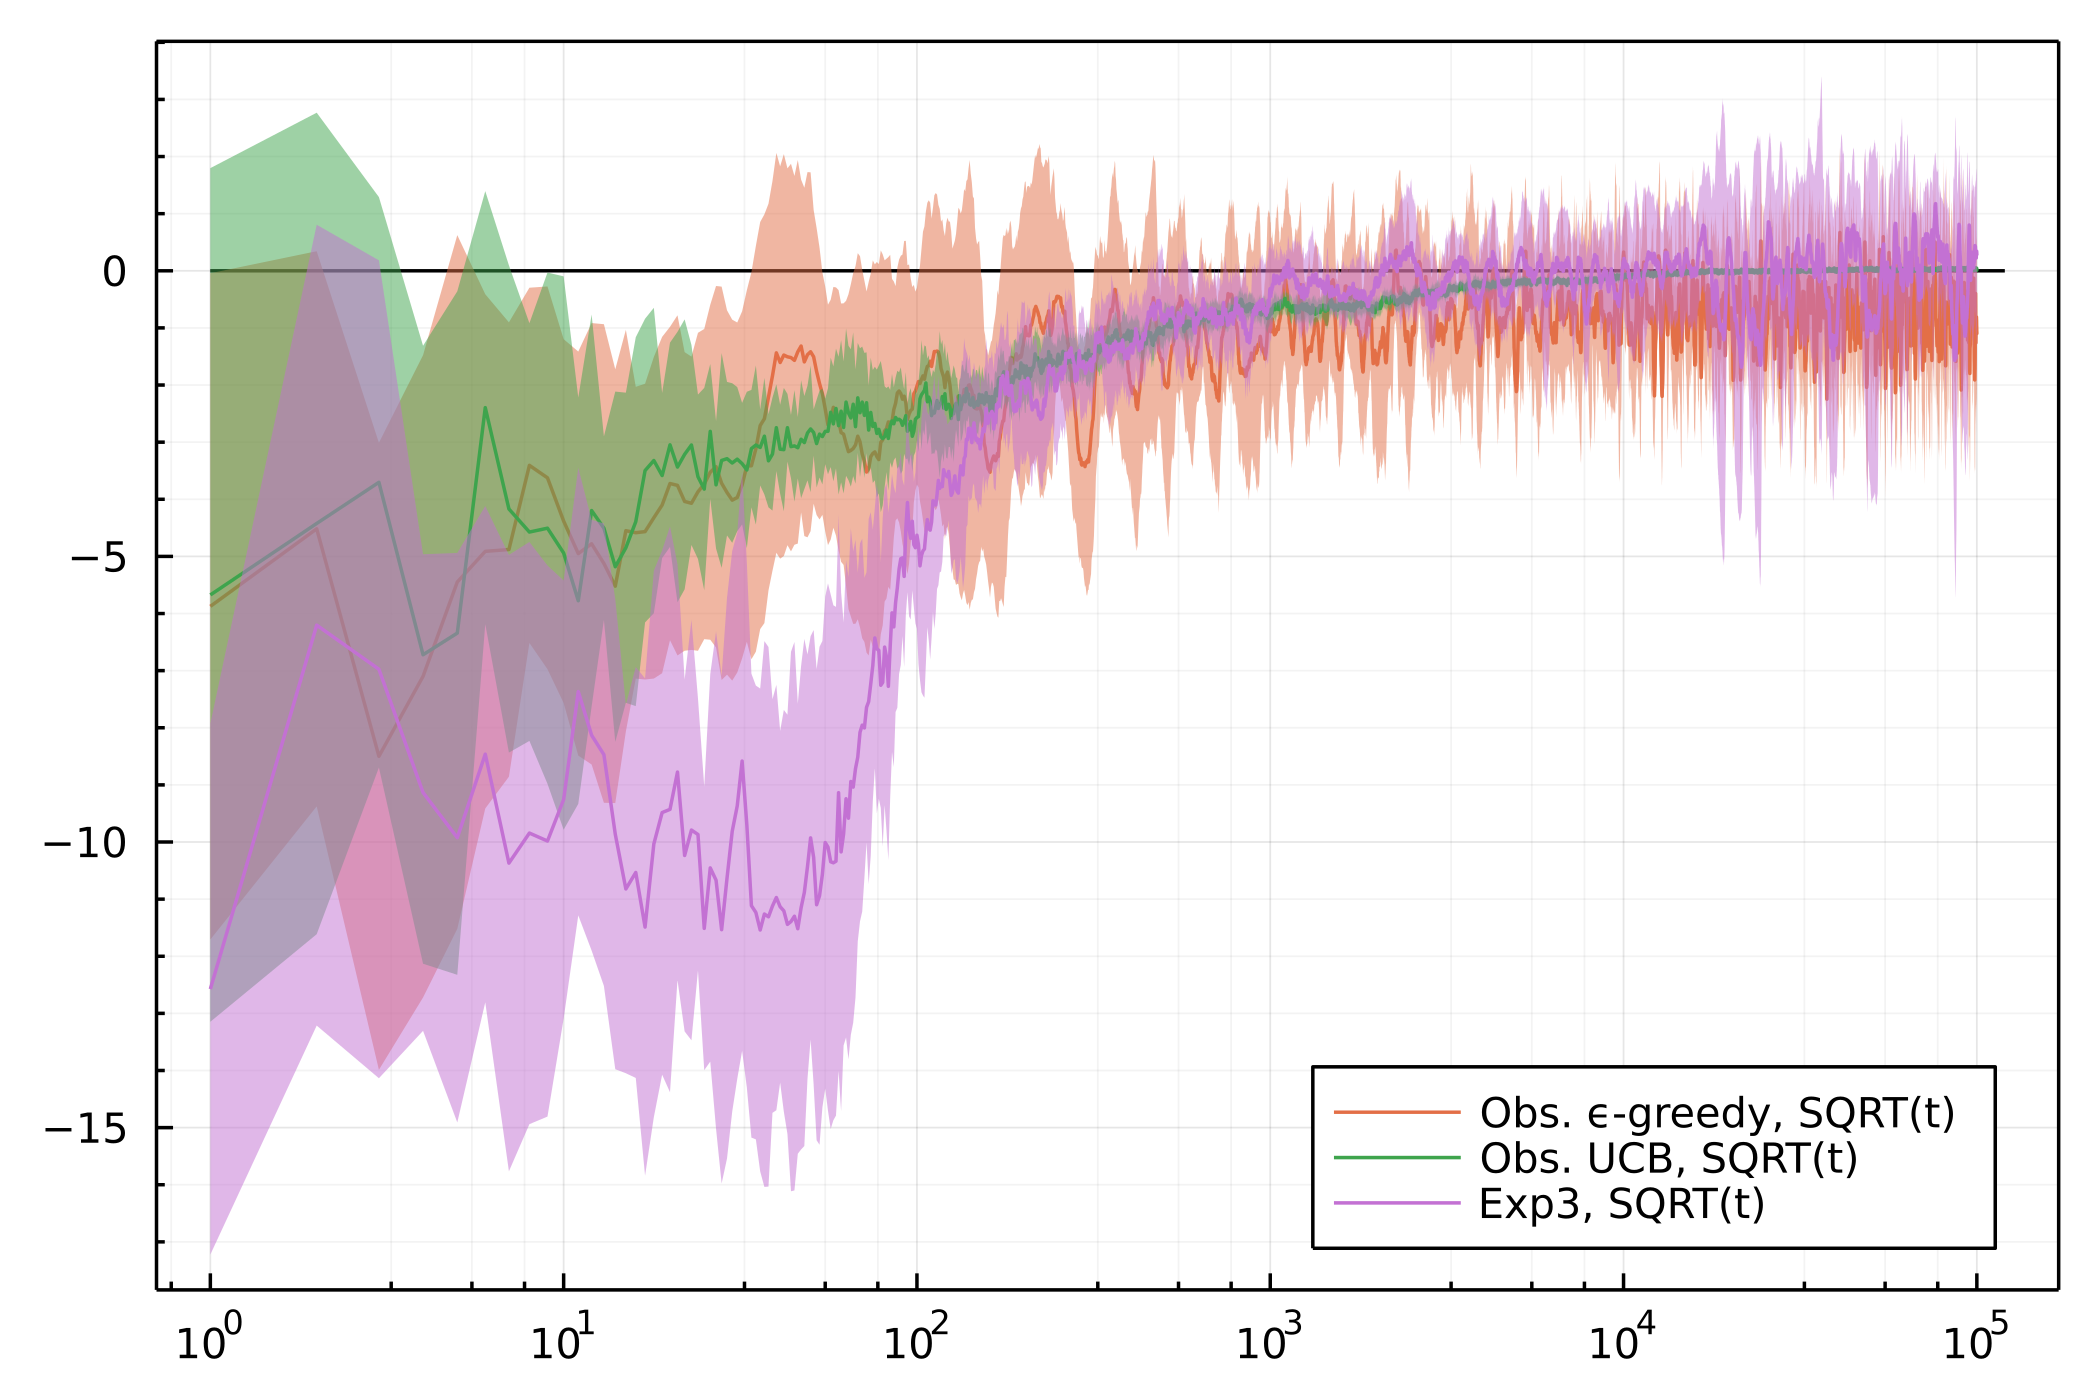
\includegraphics[width=1\textwidth]{sg/best/tag_3_01_ObservableEpsilonGreedy_ObservableUCB_Exp3_SqrtT_3_3.png}
        \caption{Observable bandits with $\sqrtt$ step}
        \label{exp:sg:best:301:33:obs:sqrt}
    \end{subfigure}
    \caption[Comparison of three best bandits and their observable counterparts on \tagname{3}{01}]{
        This quartet of figures studies development of deviation of learned values from the value iteration result over time.
        The comparison is made on a \textbf{Tag} instance \tagname{3}{01} in a mixed-strategy state $s = \left(3, 3\right)$ for the three best bandits from previous comparisons, $\epsilon$-greedy, UCB and Exp3, in combination with the two step functions, $\lint$ and $\sqrtt$.
        The top half compares the standard bandits together, the bottom half their observable complements.
    }
    \label{exp:sg:best:301:33}
\end{figure}
In this state \reffig{exp:sg:best:301:33}, the Exp3 algorithm is superior to the standard versions without adversary's average play.
Even though it falls behind at the beginning and despite the large fluctuations with the $\sqrtt$ step, it eventually overcomes the other two in convergence.
Standard UCB and $\epsilon$-greedy perform approximately the same, but UCB is more resistant to the fluctuations caused by the weighted step.
The observable UCB, however, catches up to the Exp3 algorithm and does not oscillate afterwards, observable $\epsilon$-greedy follow close behind.

The second state is $s = \left(4, 4\right)$ of the instance \tagname{3}{02} \reffig{exp:sg:games:tag:examples:32}.
\begin{figure}[ht]
    \begin{subfigure}[t]{0.45\linewidth}
        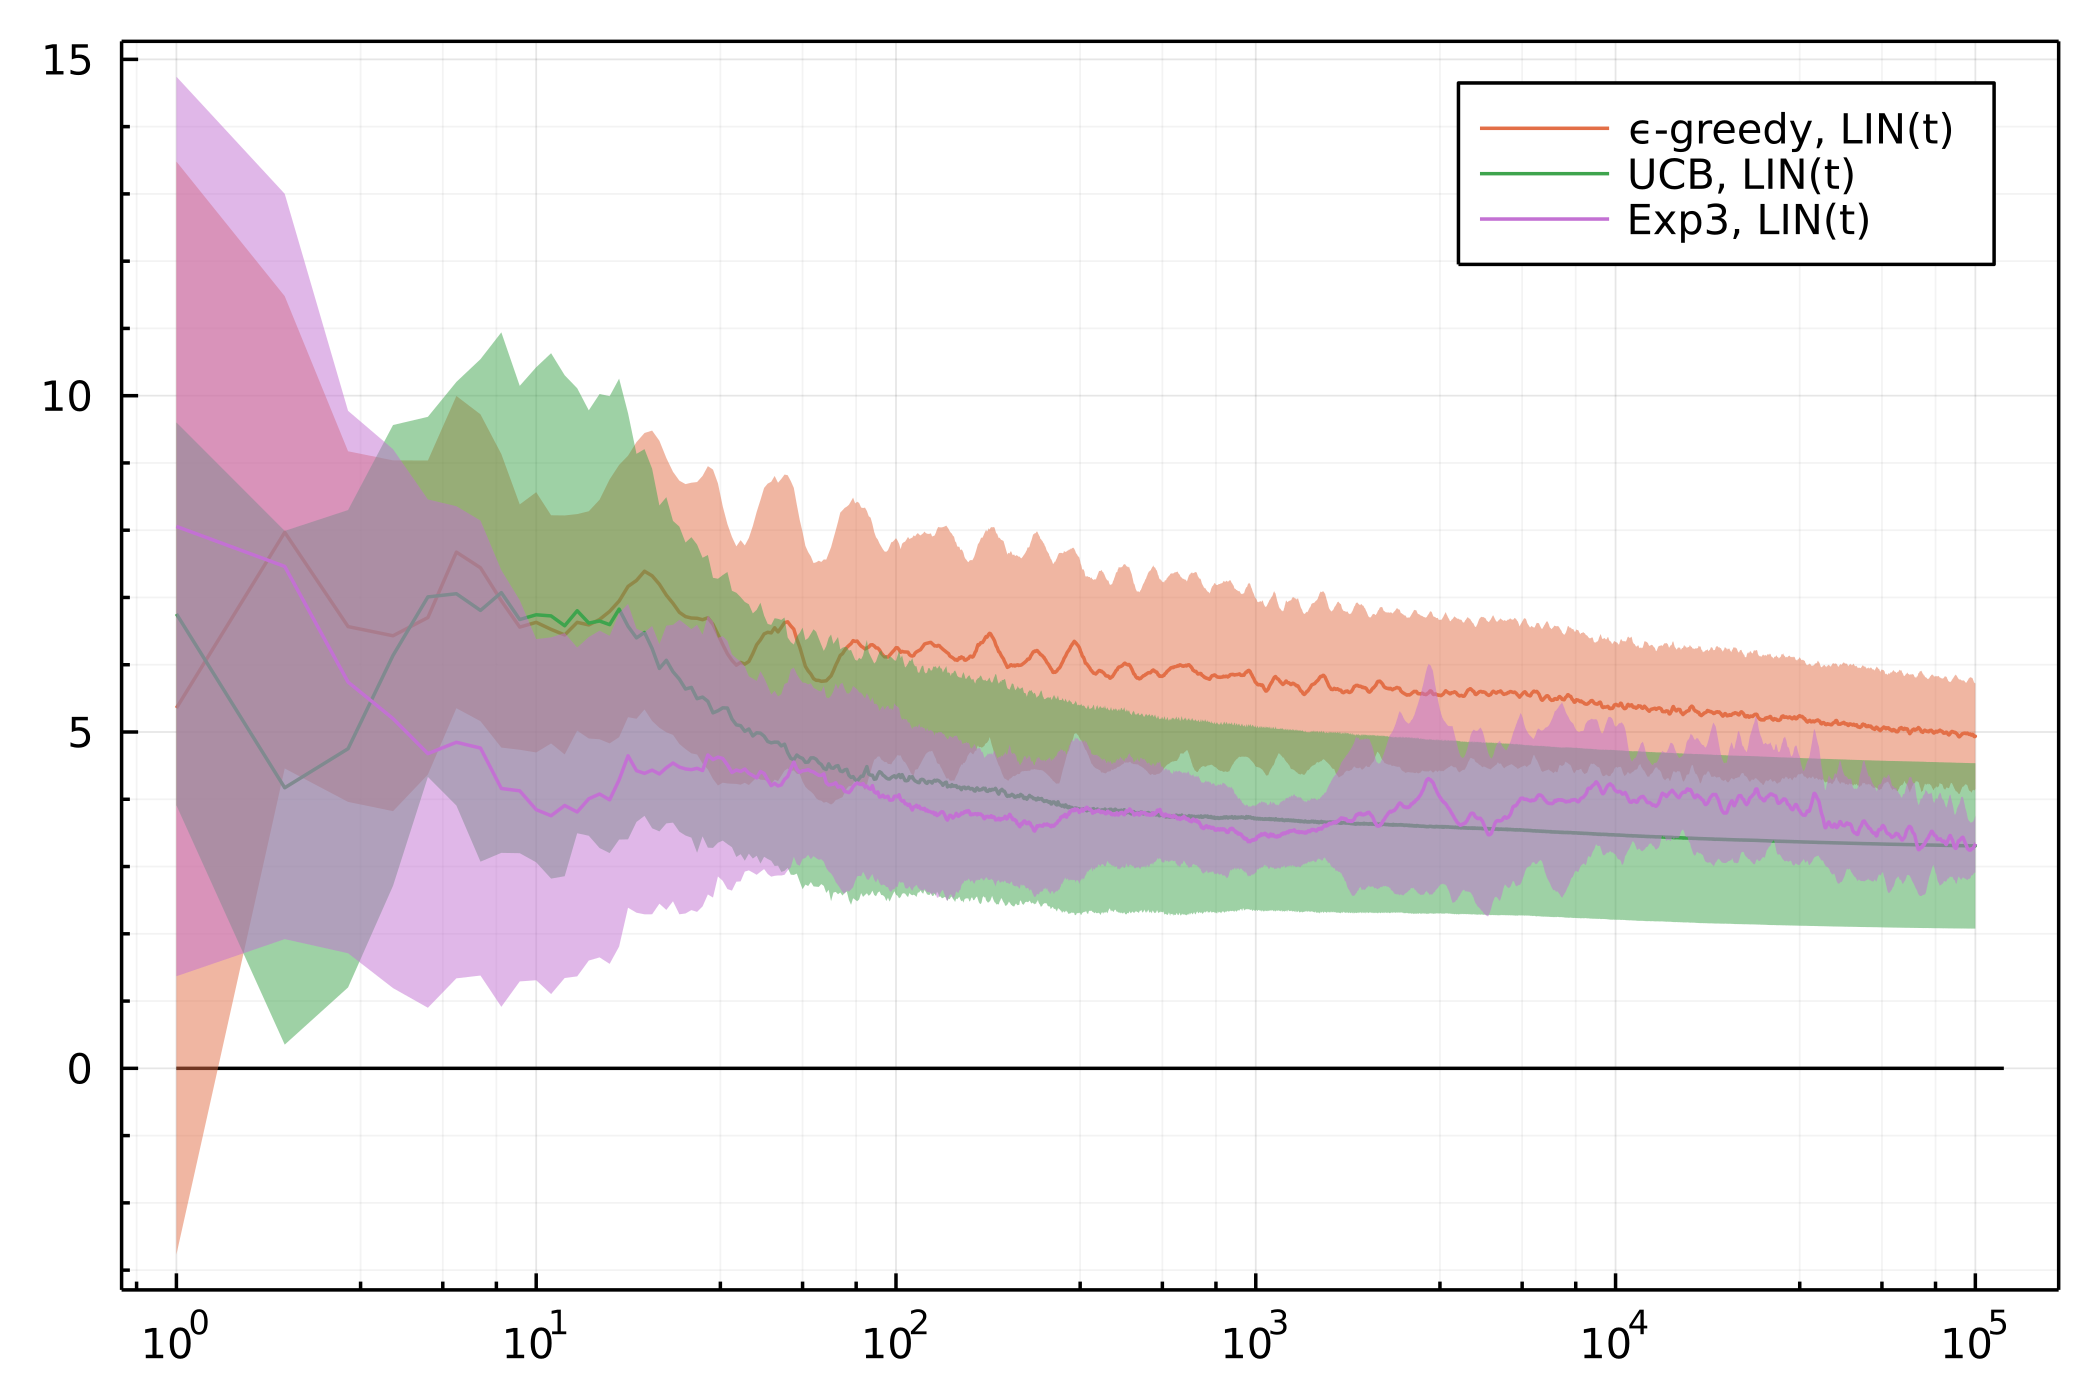
\includegraphics[width=1\textwidth]{sg/best/tag_3_02_EpsilonGreedy_UCB_Exp3_LinT_4_4.png}
        \caption{Standard bandits with $\lint$ step}
        \label{exp:sg:best:302:44:std:lin}
    \end{subfigure}
    \hfill
    \begin{subfigure}[t]{0.45\linewidth}
        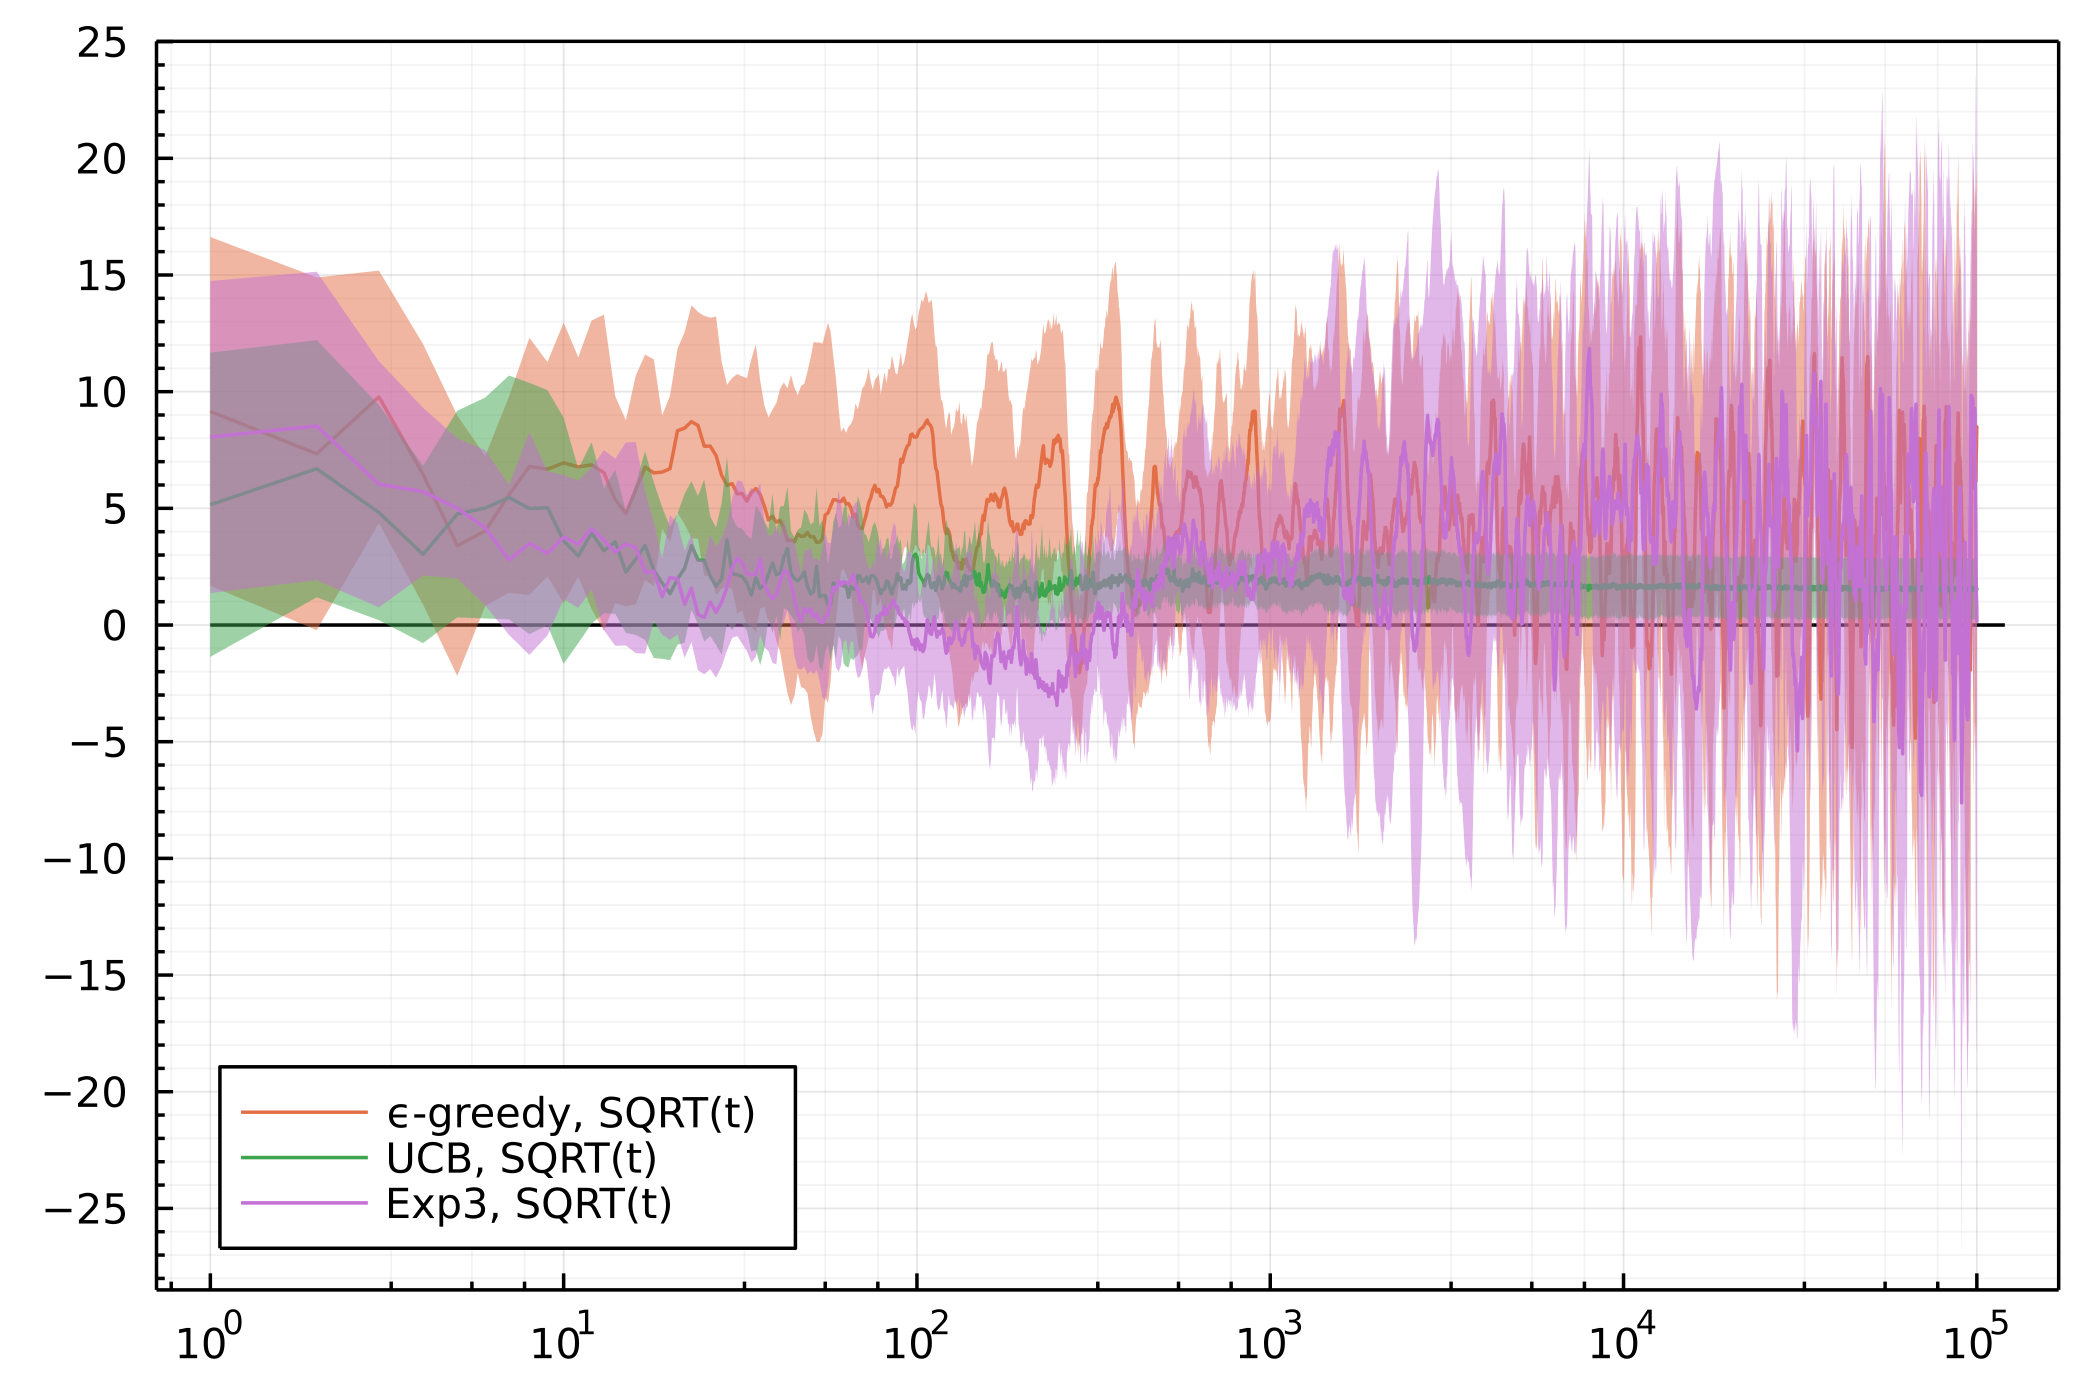
\includegraphics[width=1\textwidth]{sg/best/tag_3_02_EpsilonGreedy_UCB_Exp3_SqrtT_4_4.png}
        \caption{Standard bandits with $\sqrtt$ step}
        \label{exp:sg:best:302:44:std:sqrt}
    \end{subfigure}
    \begin{subfigure}[t]{0.45\linewidth}
        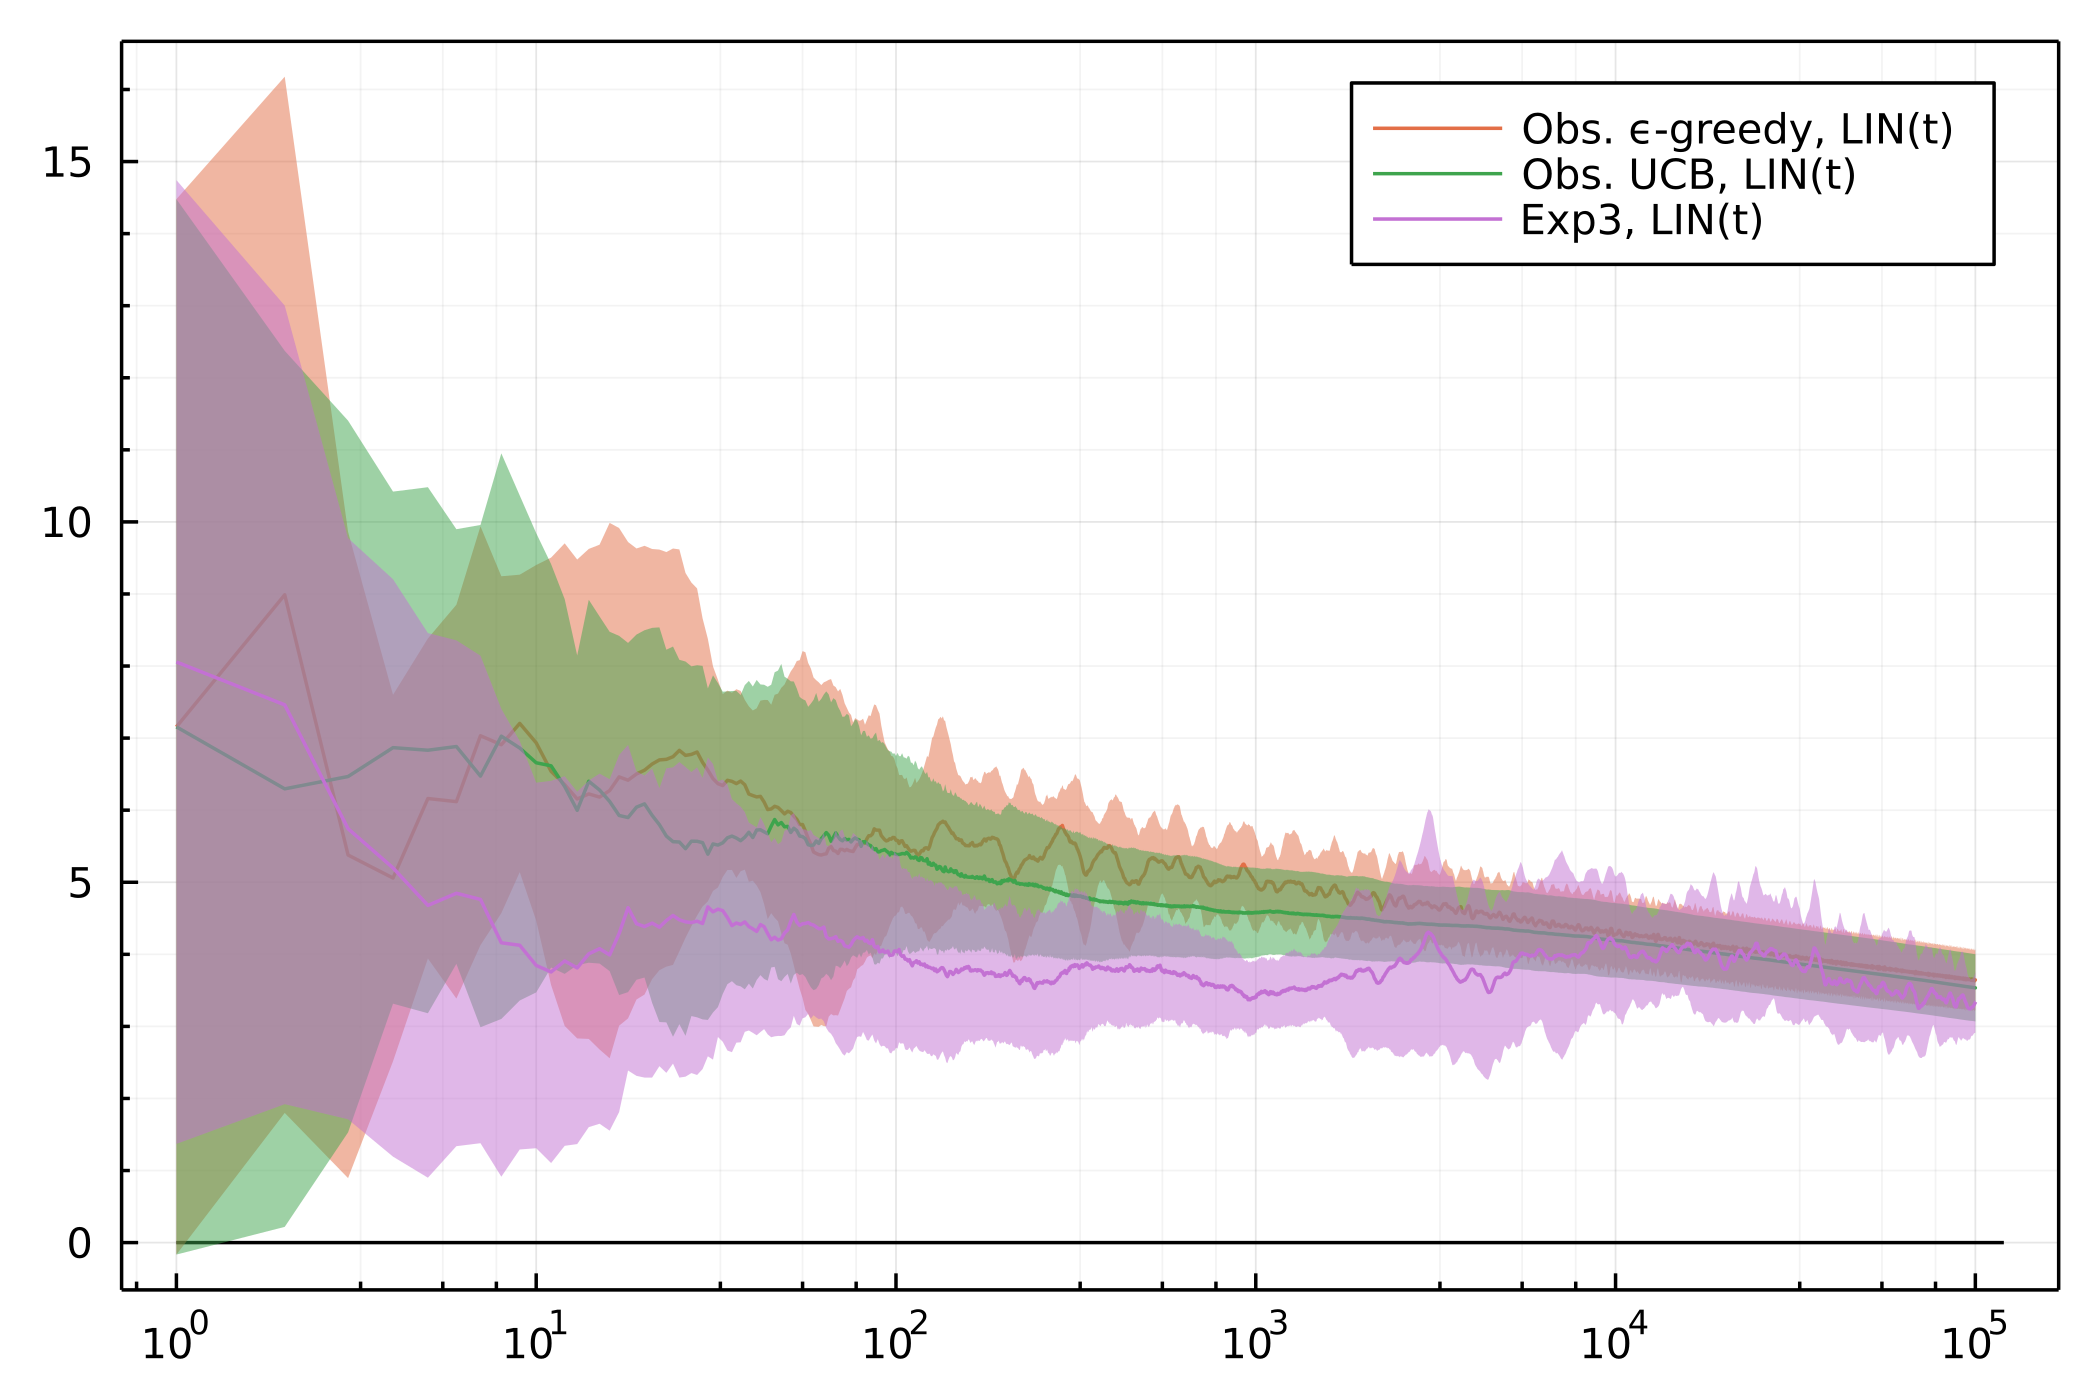
\includegraphics[width=1\textwidth]{sg/best/tag_3_02_ObservableEpsilonGreedy_ObservableUCB_Exp3_LinT_4_4.png}
        \caption{Observable bandits with $\lint$ step}
        \label{exp:sg:best:302:44:obs:lint}
    \end{subfigure}
    \hfill
    \begin{subfigure}[t]{0.45\linewidth}
        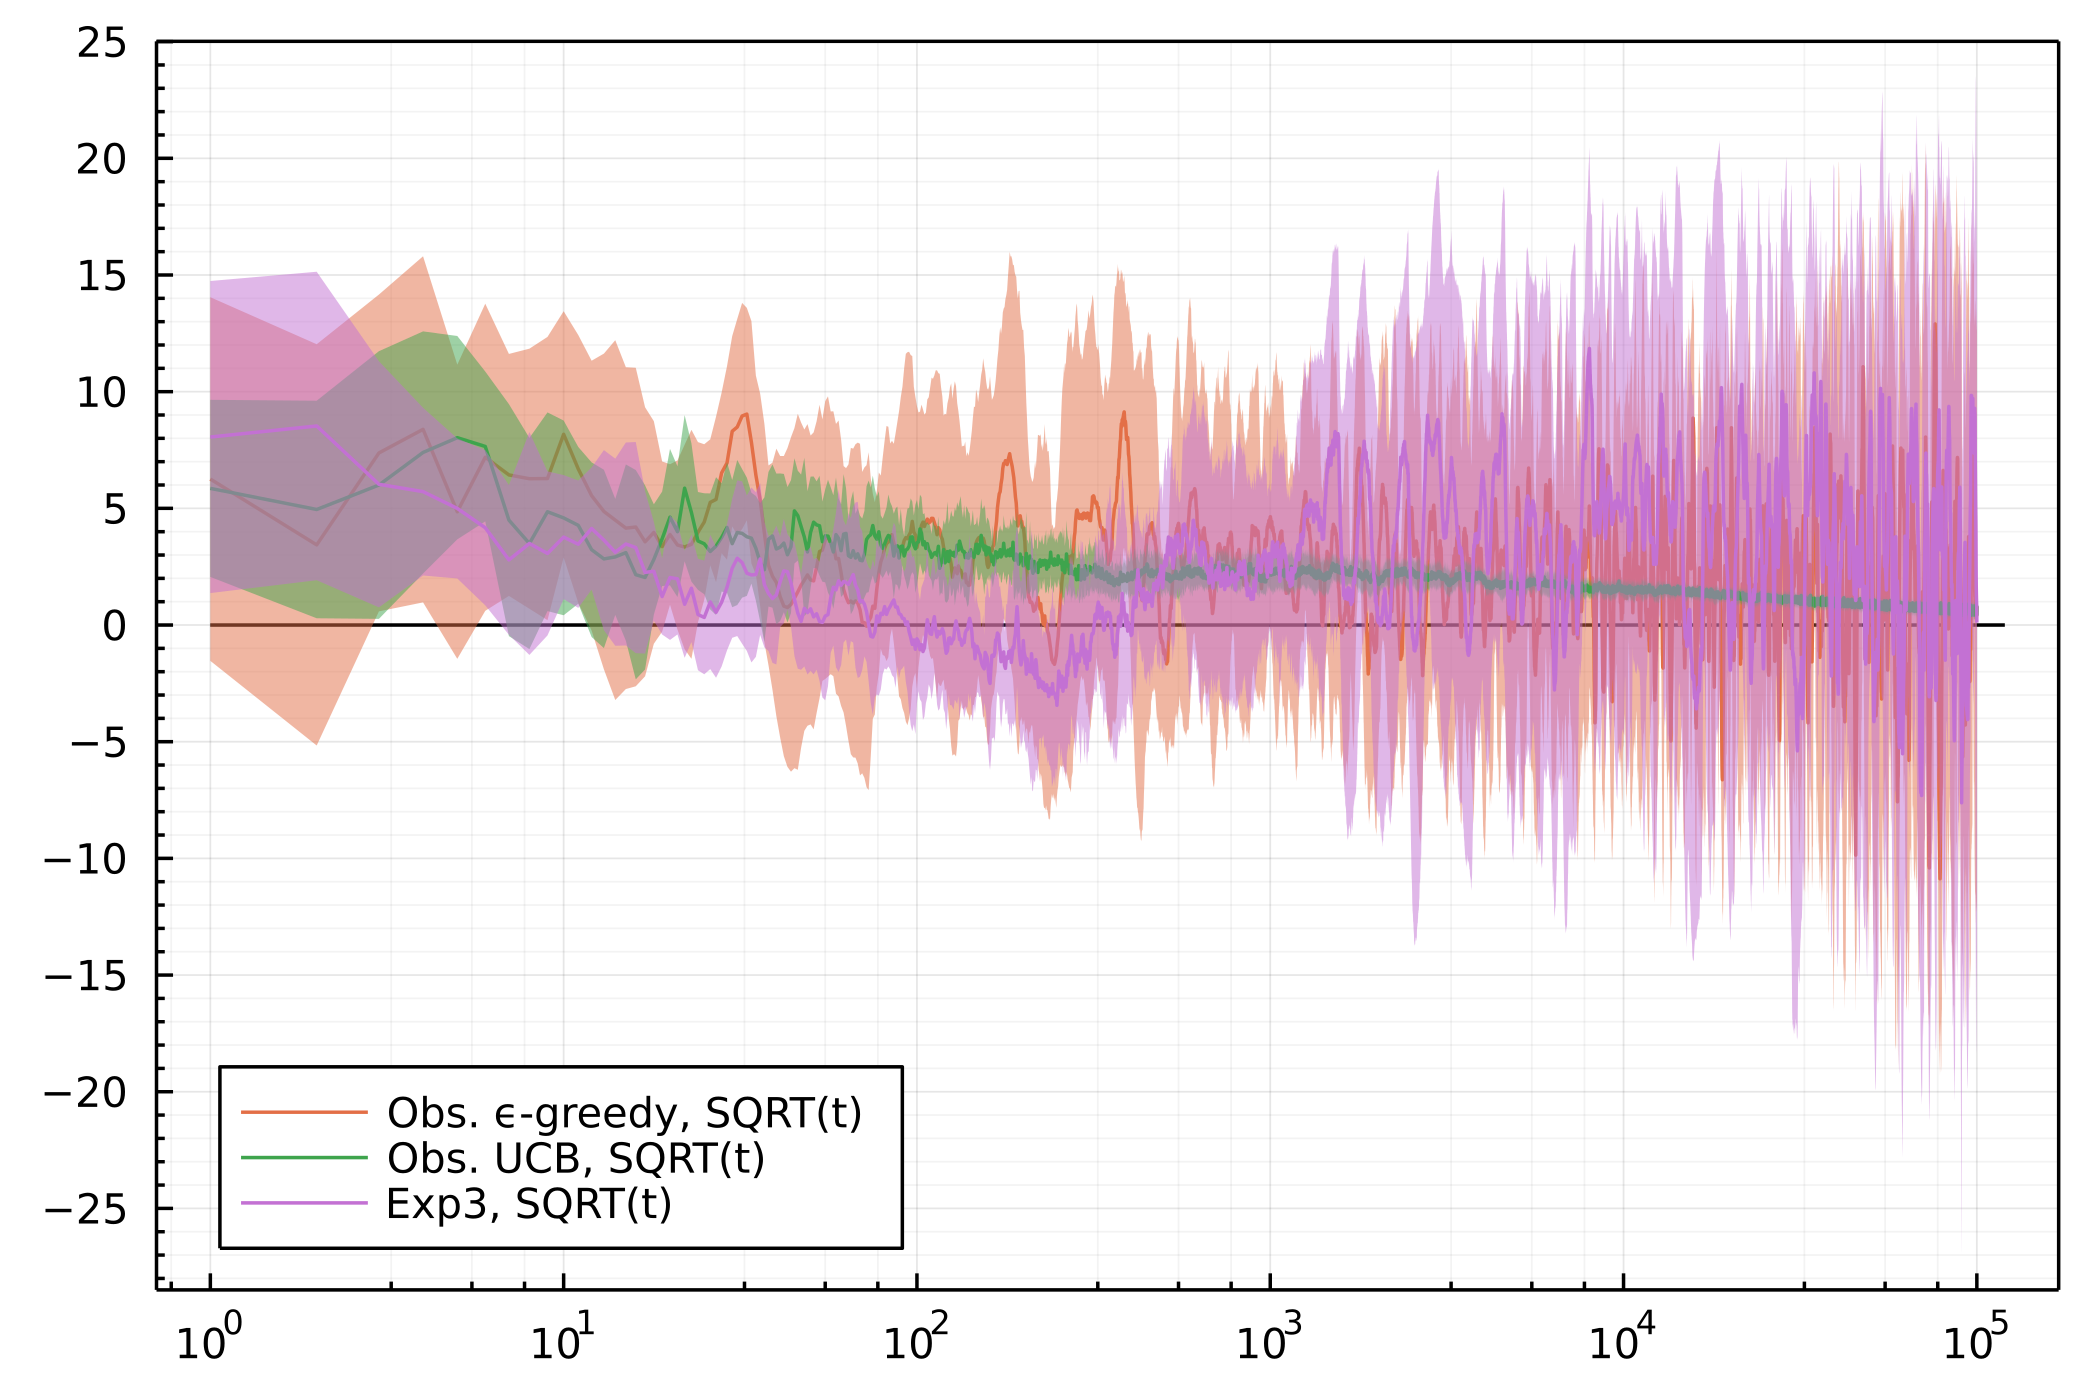
\includegraphics[width=1\textwidth]{sg/best/tag_3_02_ObservableEpsilonGreedy_ObservableUCB_Exp3_SqrtT_4_4.png}
        \caption{Observable bandits with $\sqrtt$ step}
        \label{exp:sg:best:302:44:obs:sqrt}
    \end{subfigure}
    \caption[Comparison of three best bandits and their observable counterparts on \tagname{3}{02} in a state $s = \left(4, 4\right)$]{
        This quartet of figures studies development of deviation of learned values from the value iteration result over time.
        The comparison is made on a \textbf{Tag} instance \tagname{3}{02} in a mixed-strategy state $s = \left(4, 4\right)$ for the three best bandits from previous comparisons, $\epsilon$-greedy, UCB and Exp3, in combination with the two step functions, $\lint$ and $\sqrtt$.
        The top half compares the standard bandits together, the bottom half their observable complements.
    }
    \label{exp:sg:best:302:44}
\end{figure}
Here \reffig{exp:sg:best:302:44}, all the bandits converge very slowly with the $\lint$ step.
Moreover, the non-observable variants seem to converge to some suboptimal values, even though, after many more iterations, the Exp3 algorithm appears that it would approach the optimum closer.
The observable bandits converge as slowly as the standard ones, but the trend suggests further decrease of the deviation from the value of the game for more iterations.
With this step function, these three algorithms are comparable.

When it comes to $\sqrtt$, the situation dramatically improves.
Especially the average play UCB performs very well as it converges close to the real value and does not fluctuate afterwards.
The other standard bandits converge to another value and oscillate around it, while the observable ones converge to the optimum.
The fluctuations are enormous, when intersected by a line.

The situation \reffig{exp:sg:best:302:14} for the third discussed state $s = \left(1, 4\right)$ of the instance \tagname{3}{02} \reffig{exp:sg:games:tag:examples:32} is very similar to the second example with few exceptions which will be now discussed.
\begin{figure}[ht]
    \begin{subfigure}[t]{0.45\linewidth}
        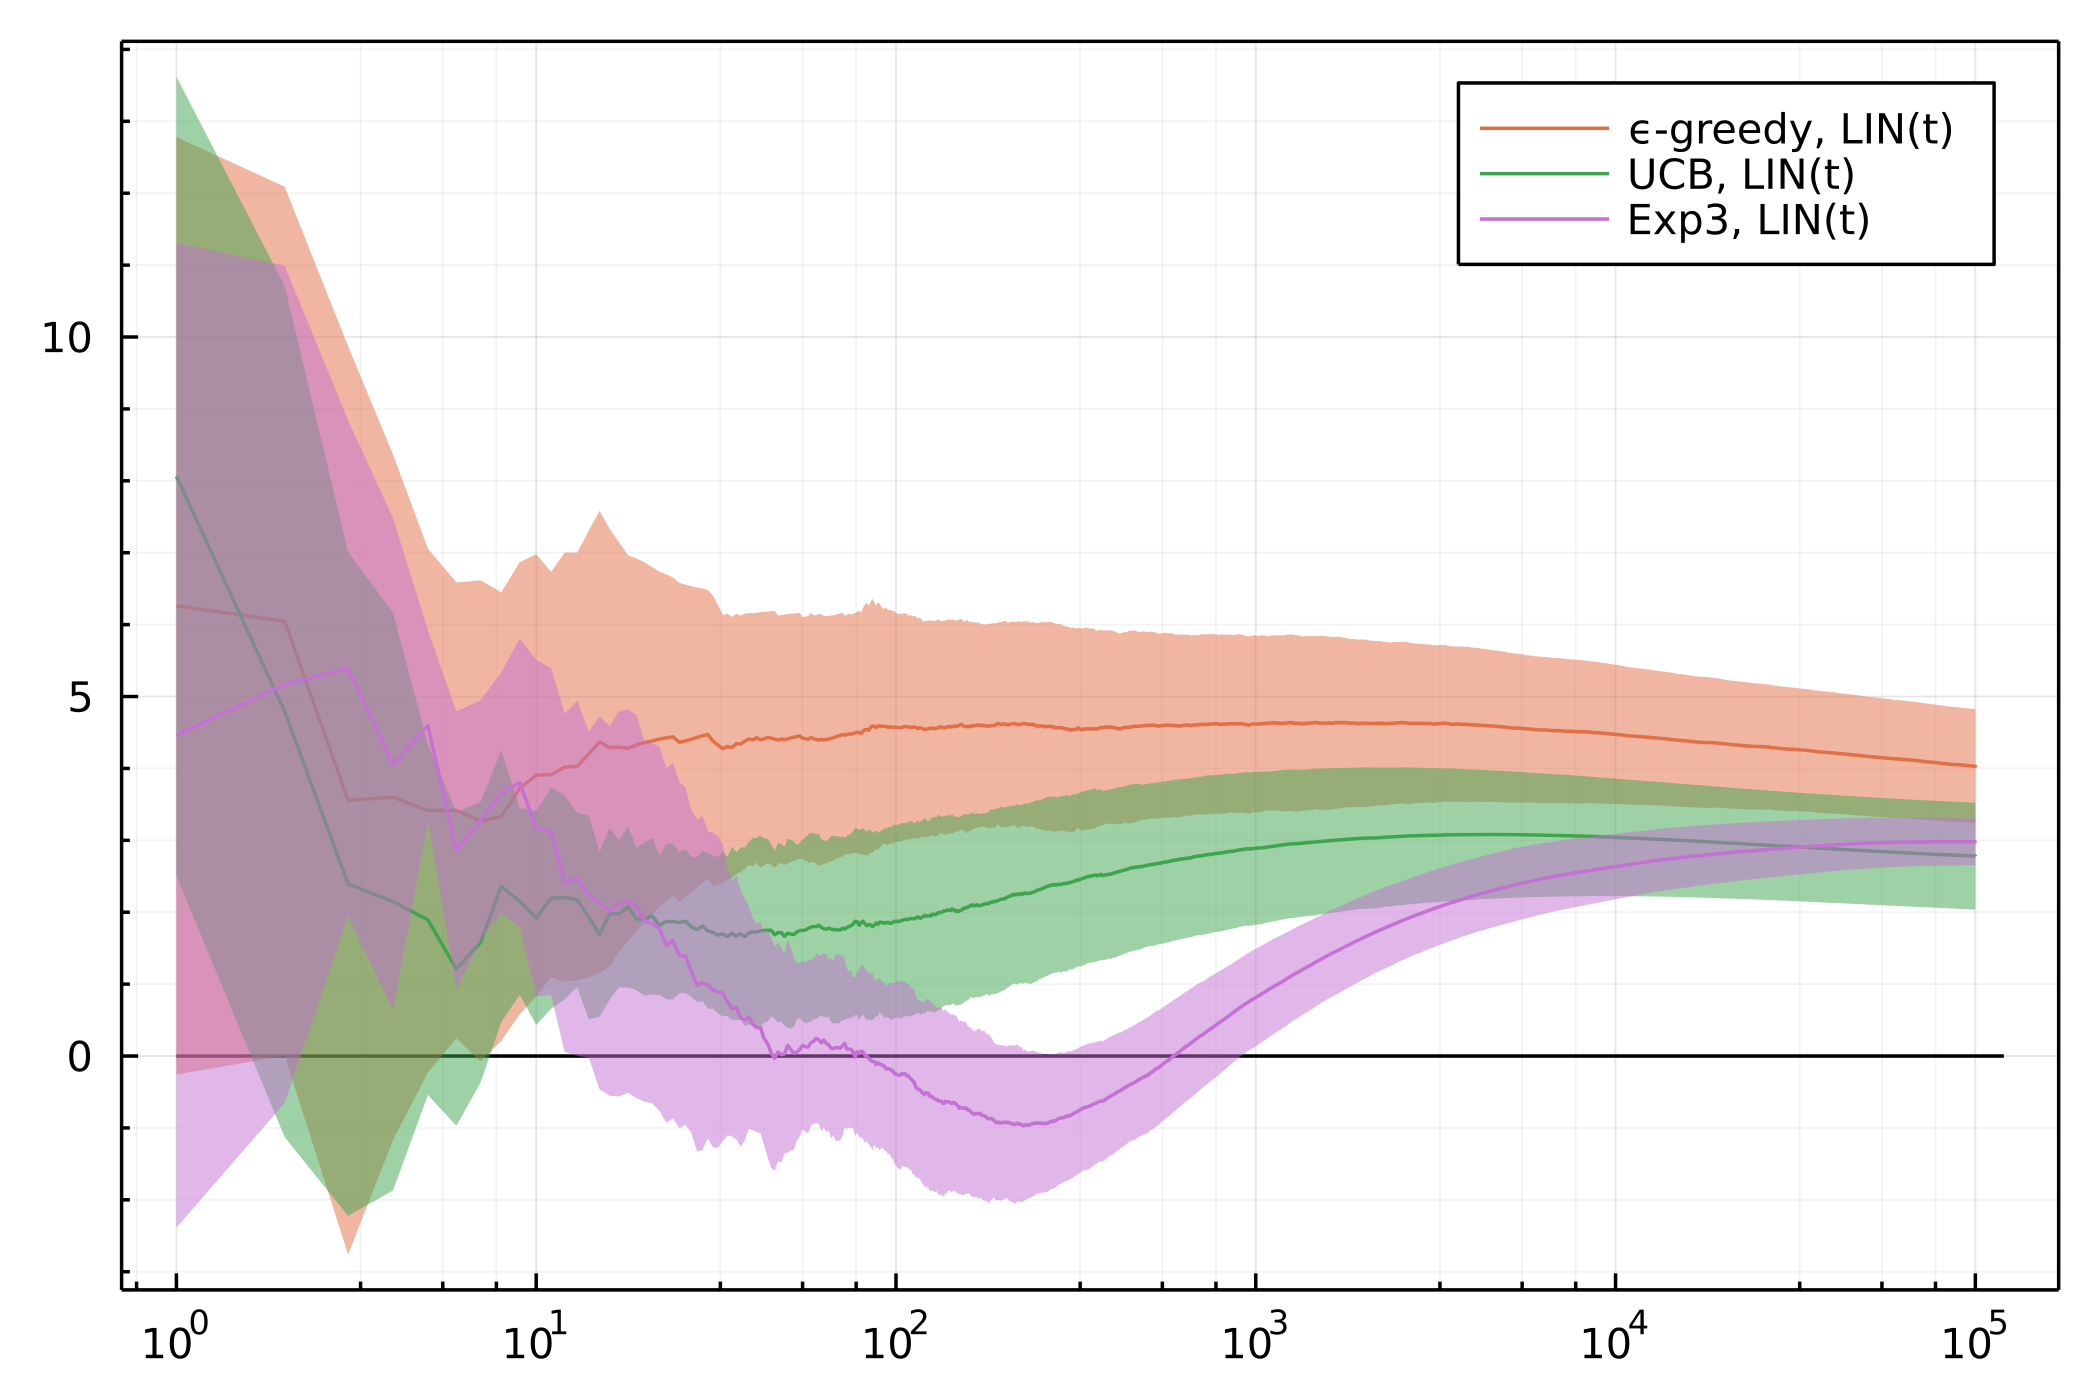
\includegraphics[width=1\textwidth]{sg/best/tag_3_02_EpsilonGreedy_UCB_Exp3_LinT_1_4.png}
        \caption{Standard bandits with $\lint$ step}
        \label{exp:sg:best:302:14:std:lin}
    \end{subfigure}
    \hfill
    \begin{subfigure}[t]{0.45\linewidth}
        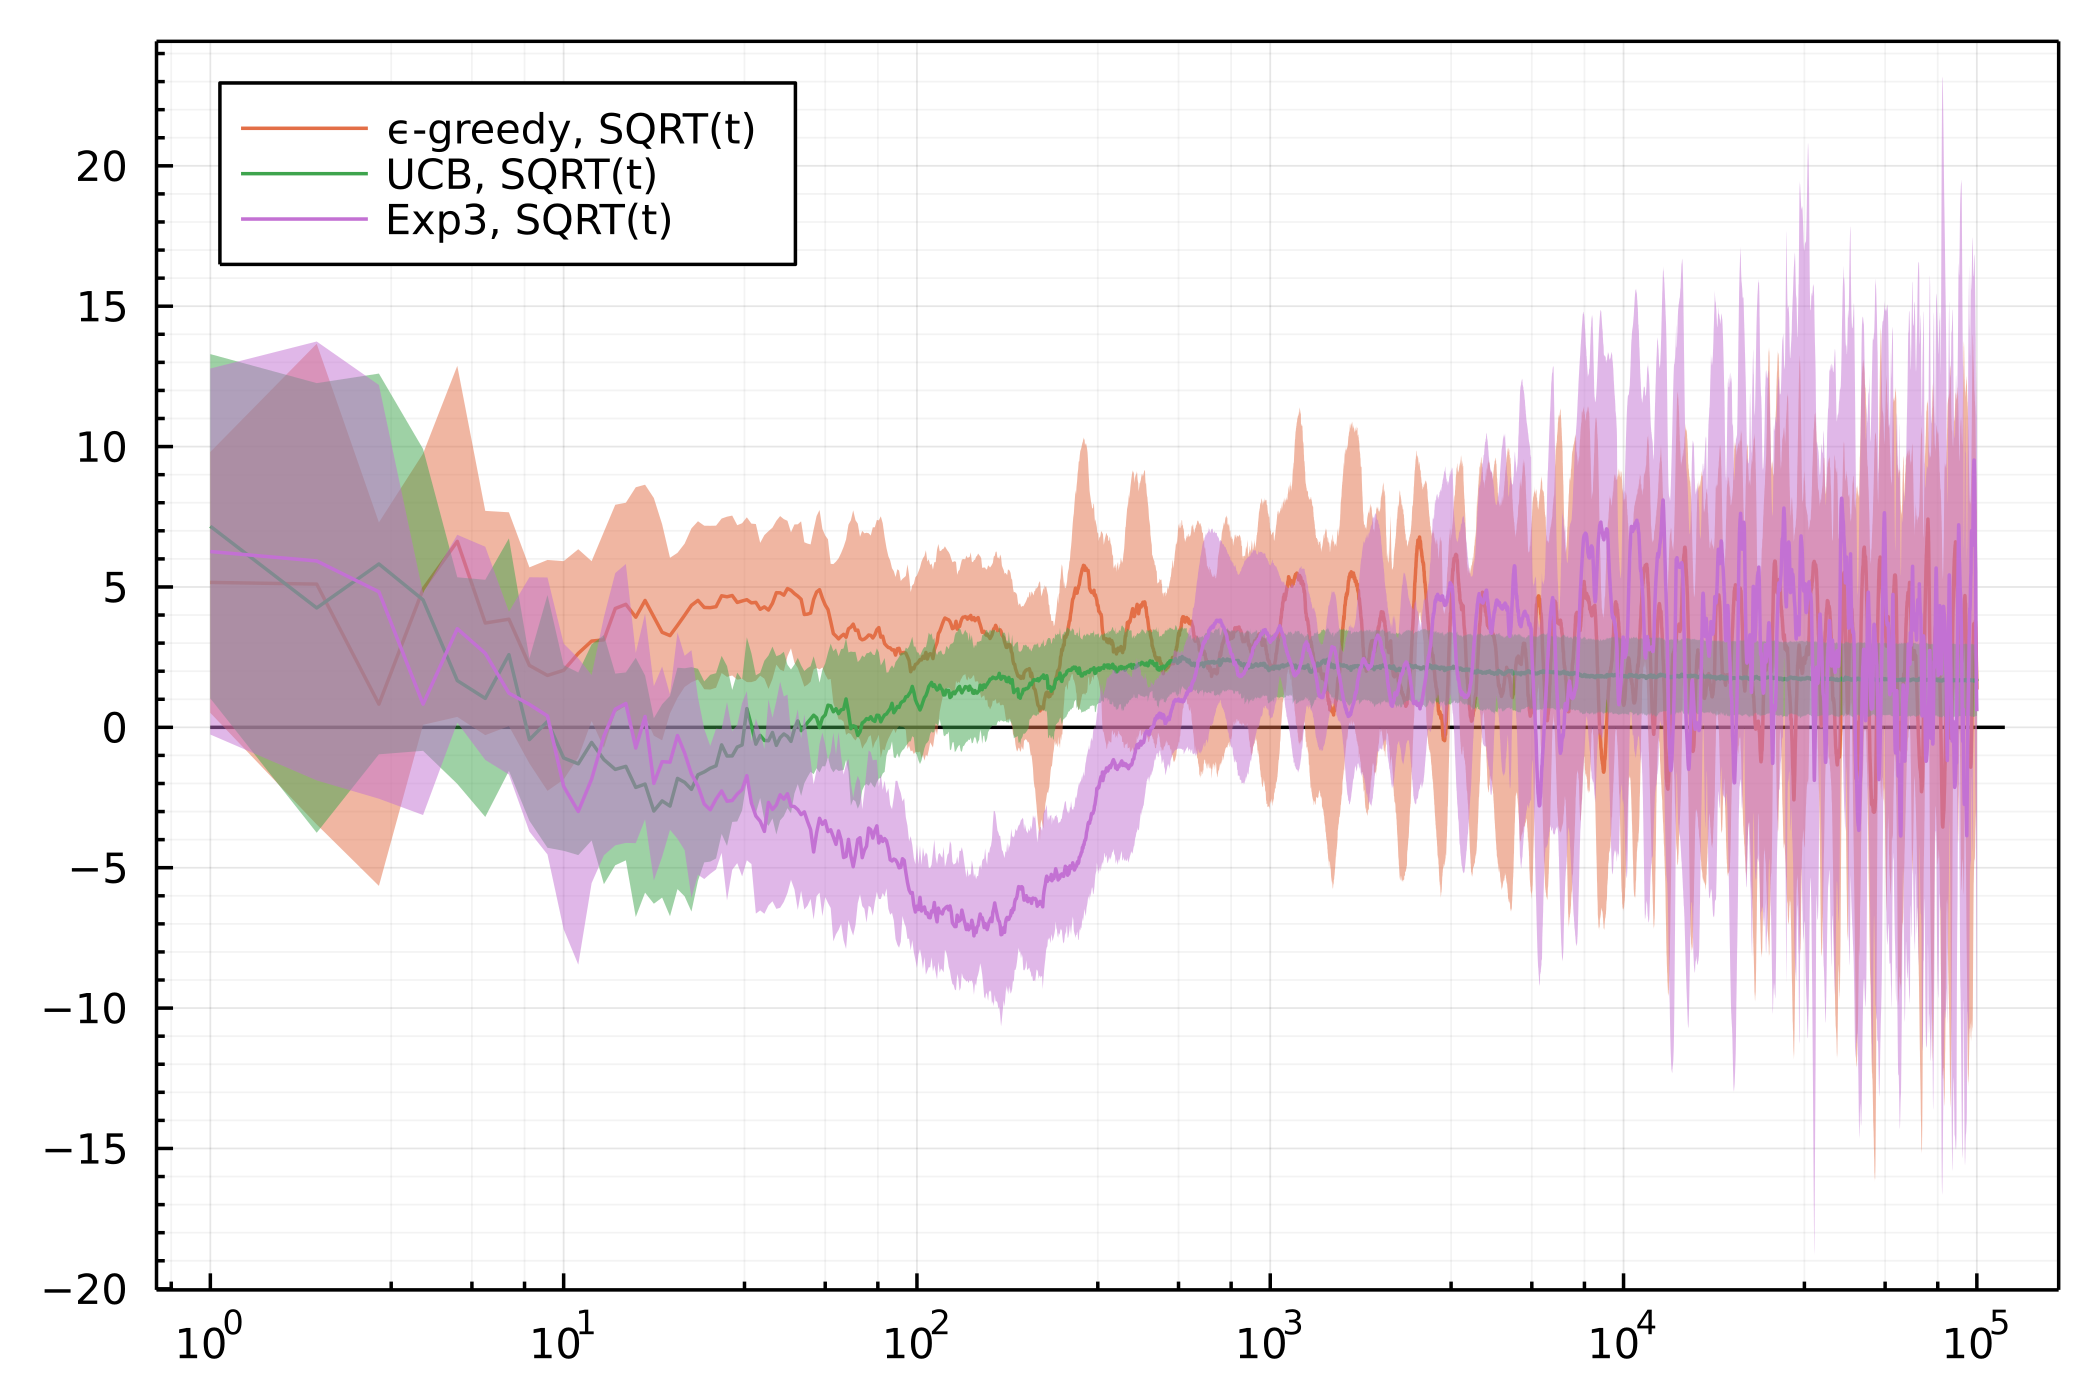
\includegraphics[width=1\textwidth]{sg/best/tag_3_02_EpsilonGreedy_UCB_Exp3_SqrtT_1_4.png}
        \caption{Standard bandits with $\sqrtt$ step}
        \label{exp:sg:best:302:14:std:sqrt}
    \end{subfigure}
    \begin{subfigure}[t]{0.45\linewidth}
        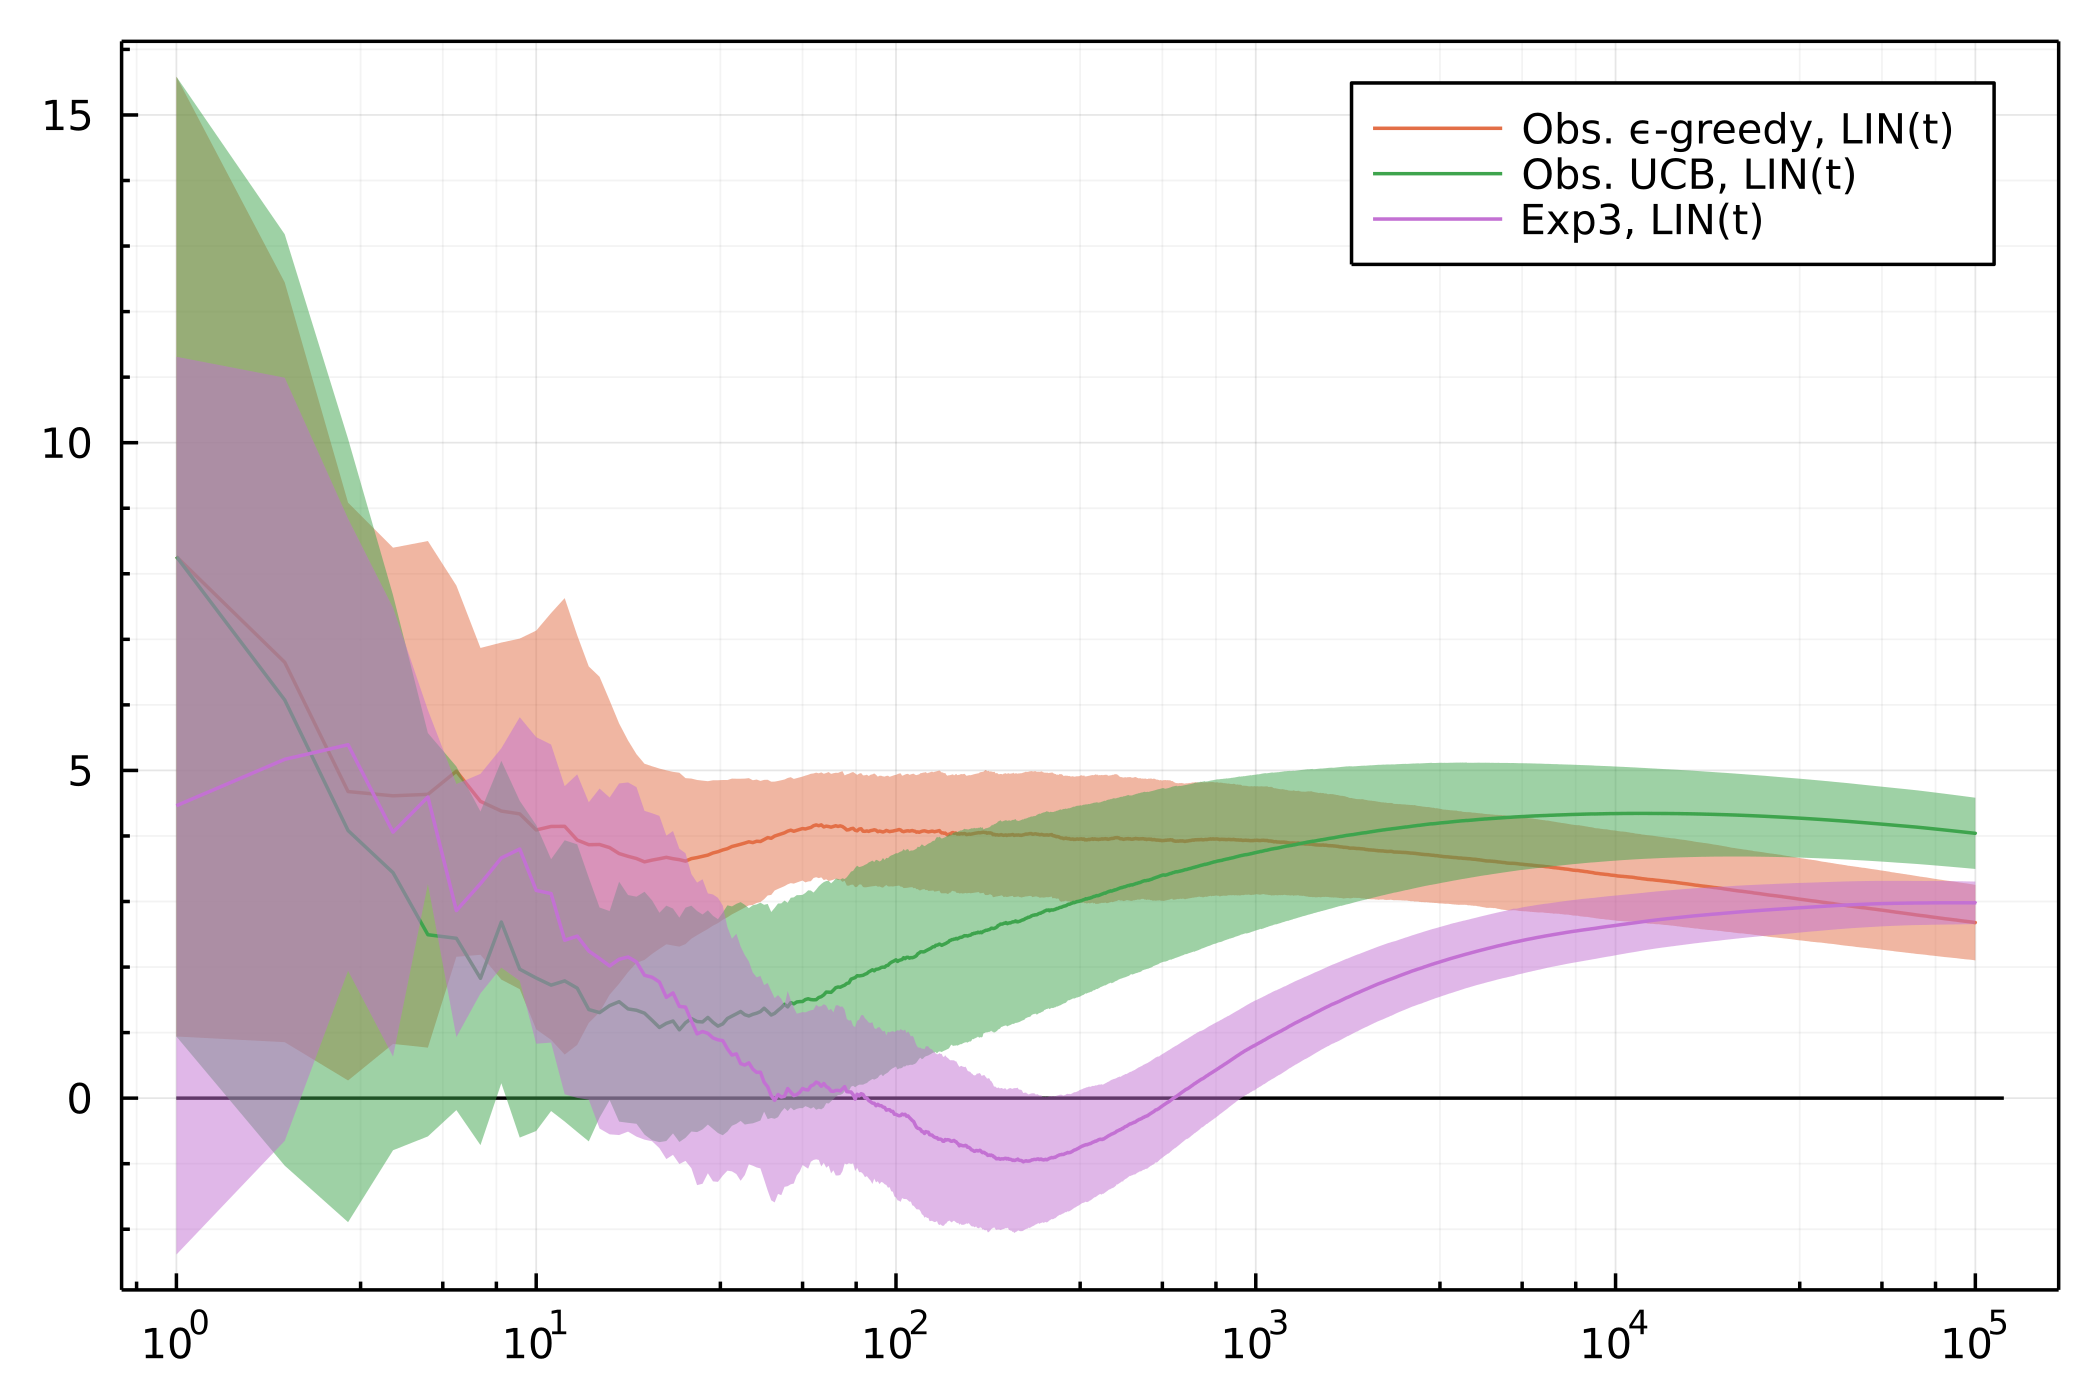
\includegraphics[width=1\textwidth]{sg/best/tag_3_02_ObservableEpsilonGreedy_ObservableUCB_Exp3_LinT_1_4.png}
        \caption{Observable bandits with $\lint$ step}
        \label{exp:sg:best:302:14:obs:lint}
    \end{subfigure}
    \hfill
    \begin{subfigure}[t]{0.45\linewidth}
        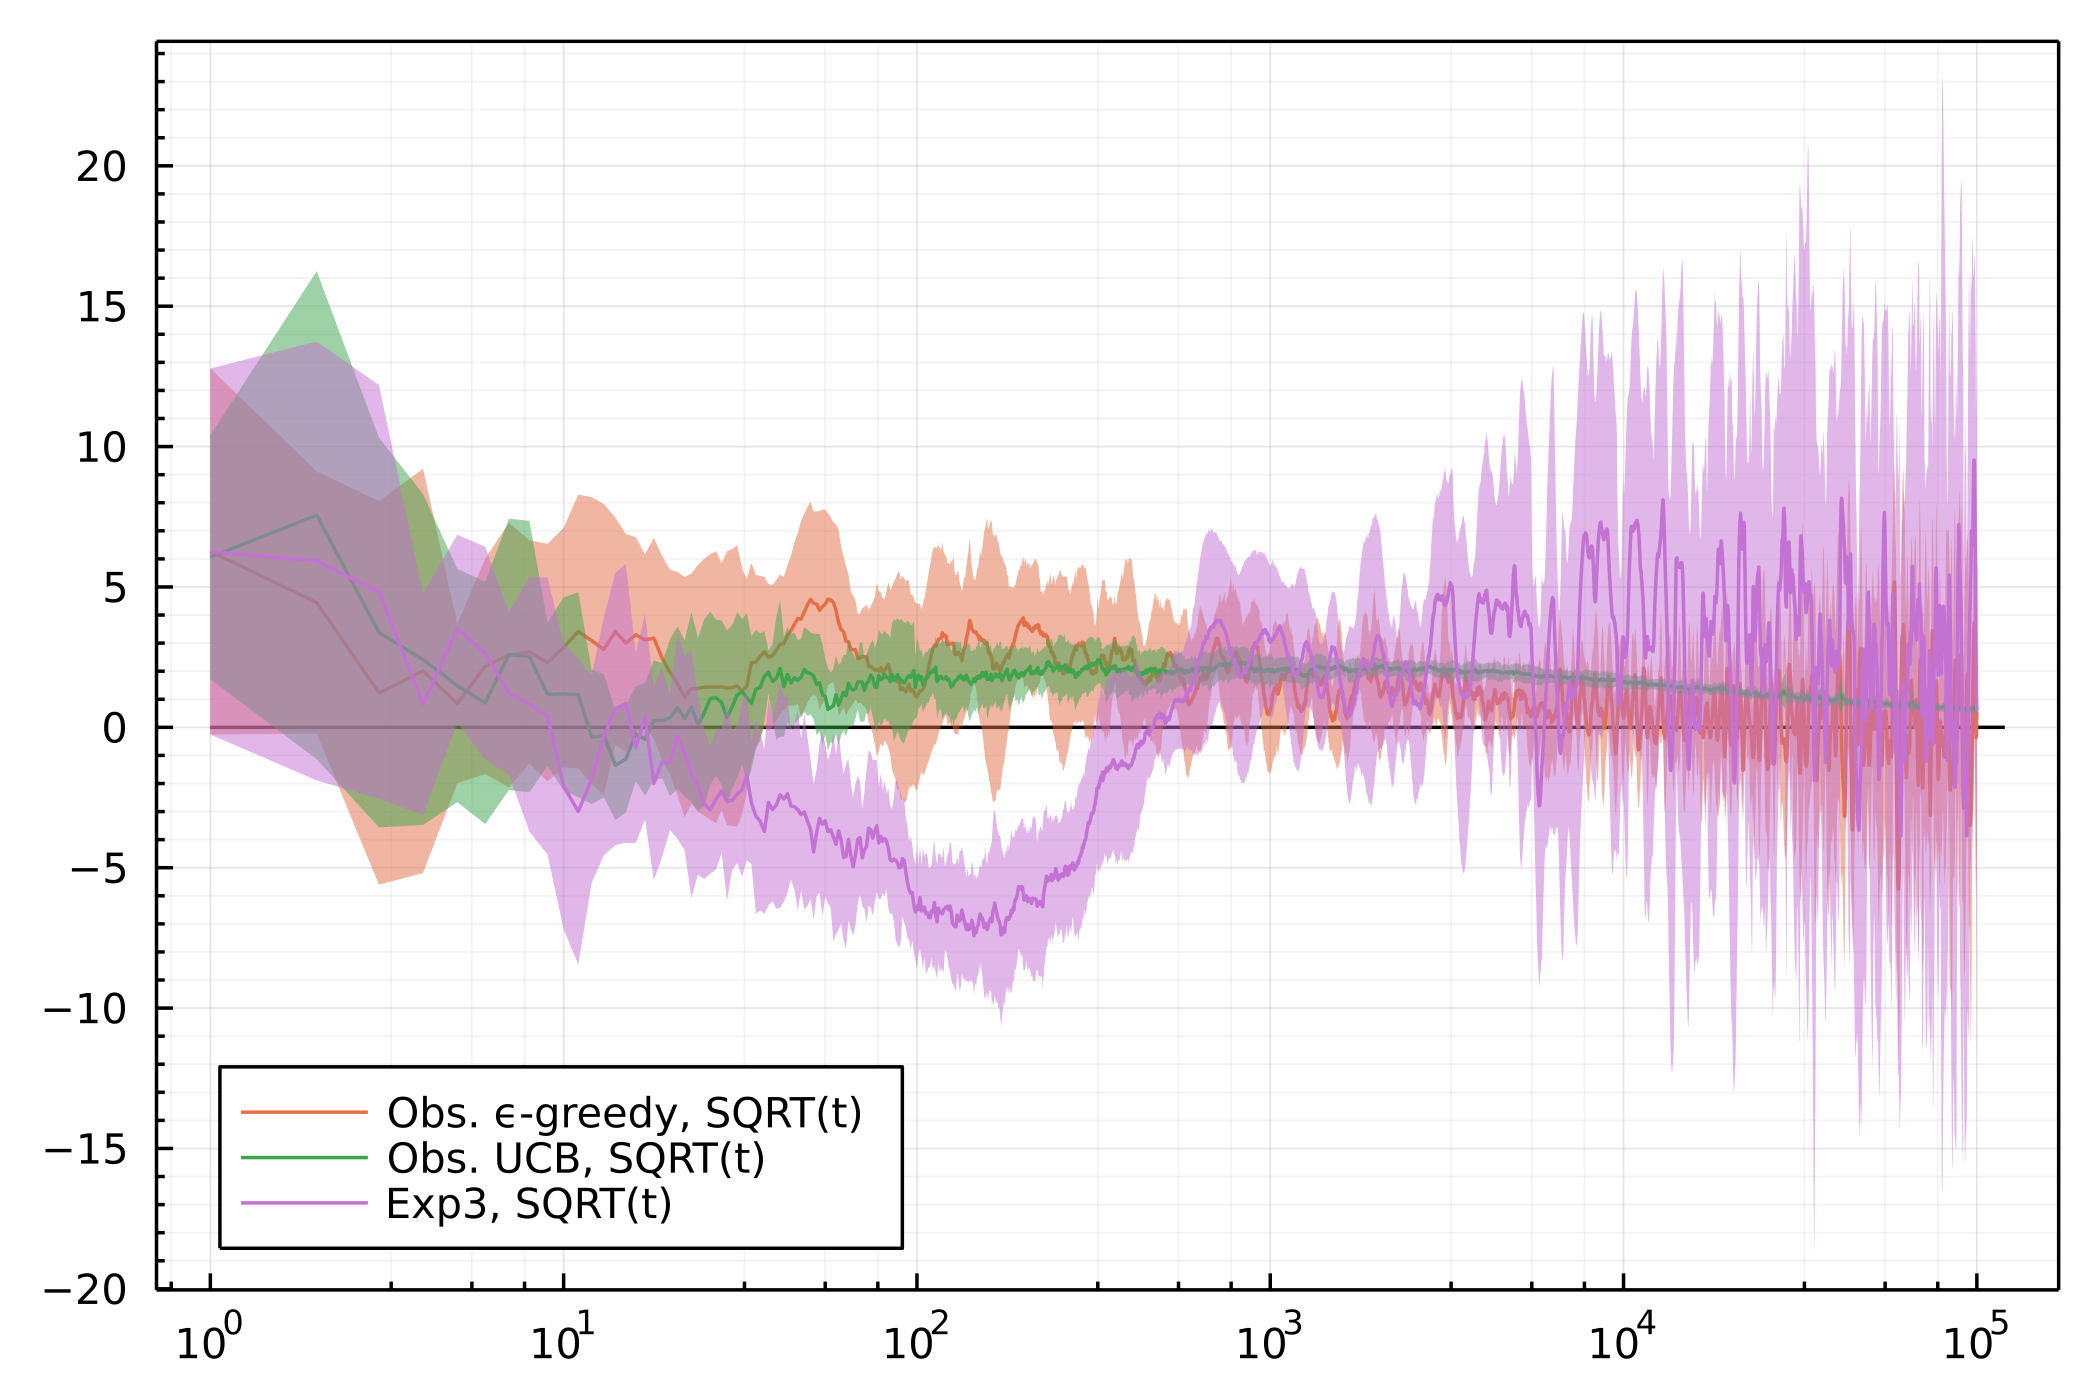
\includegraphics[width=1\textwidth]{sg/best/tag_3_02_ObservableEpsilonGreedy_ObservableUCB_Exp3_SqrtT_1_4.png}
        \caption{Observable bandits with $\sqrtt$ step}
        \label{exp:sg:best:302:14:obs:sqrt}
    \end{subfigure}
    \caption[Comparison of three best bandits and their observable counterparts on \tagname{3}{02} in a state $s = \left(1, 4\right)$]{
        This quartet of figures studies development of deviation of learned values from the value iteration result over time.
        The comparison is made on a \textbf{Tag} instance \tagname{3}{02} in a mixed-strategy state $s = \left(1, 4\right)$ for the three best bandits from previous comparisons, $\epsilon$-greedy, UCB and Exp3, in combination with the two step functions, $\lint$ and $\sqrtt$.
        The top half compares the standard bandits together, the bottom half their observable complements.
    }
    \label{exp:sg:best:302:14}
\end{figure}
The $\lint$ step performs a bit worse than in the previous case, because it approaches towards the optimal value for a while and then it diverges to another value before turning to improve again.
From the graphs it seems, that more iterations would bring the deviations even closer to $0$.
But again, the observable UCB with $\sqrtt$ step dominates the others especially in close to no fluctuations and tight standard deviation intervals.

Interestingly, the Exp3 algorithm always goes below the 0 deviation line and then again above rather than going just in one direction.
This could be tied to the two most probable joint actions which can occur in this state.
The evader can go left or down, while the tagger can hit the evader with vertical or horizontal beam.
The Exp3 thus can first explore these two pure strategies before settling to the randomized solution.

The last state is $s = \left(3, 3\right)$ from the chase instance \reffig{exp:sg:games:chase:examples:5}.
\begin{figure}[ht]
    \begin{subfigure}[t]{0.45\linewidth}
        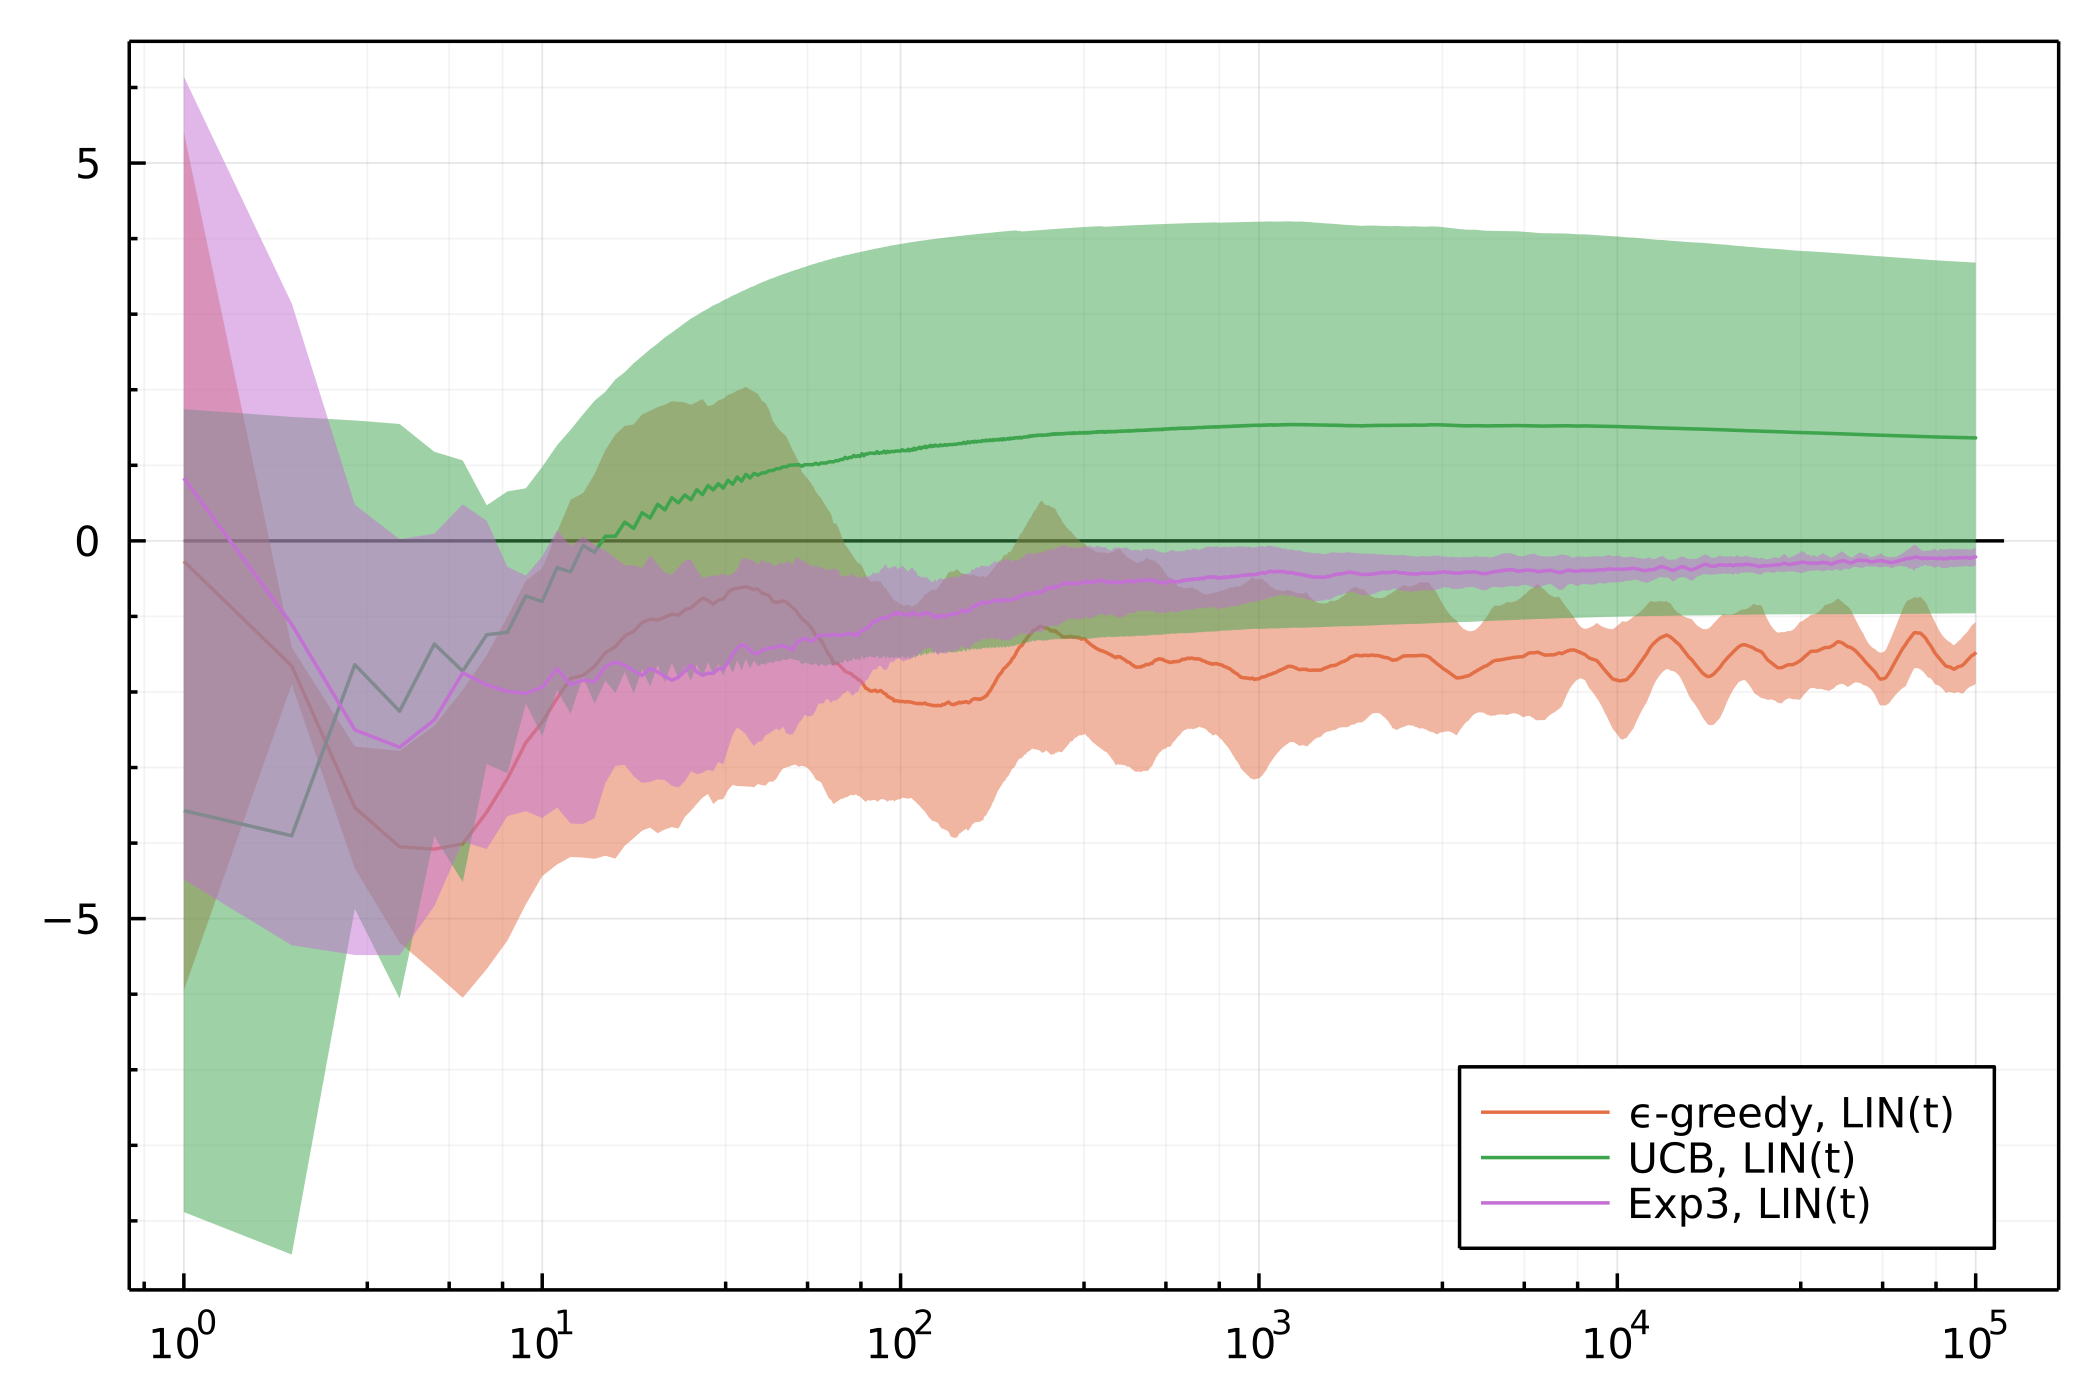
\includegraphics[width=1\textwidth]{sg/best/graphs_5_01_EpsilonGreedy_UCB_Exp3_LinT_3_3.png}
        \caption{Standard bandits with $\lint$ step}
        \label{exp:sg:best:5:33:std:lin}
    \end{subfigure}
    \hfill
    \begin{subfigure}[t]{0.45\linewidth}
        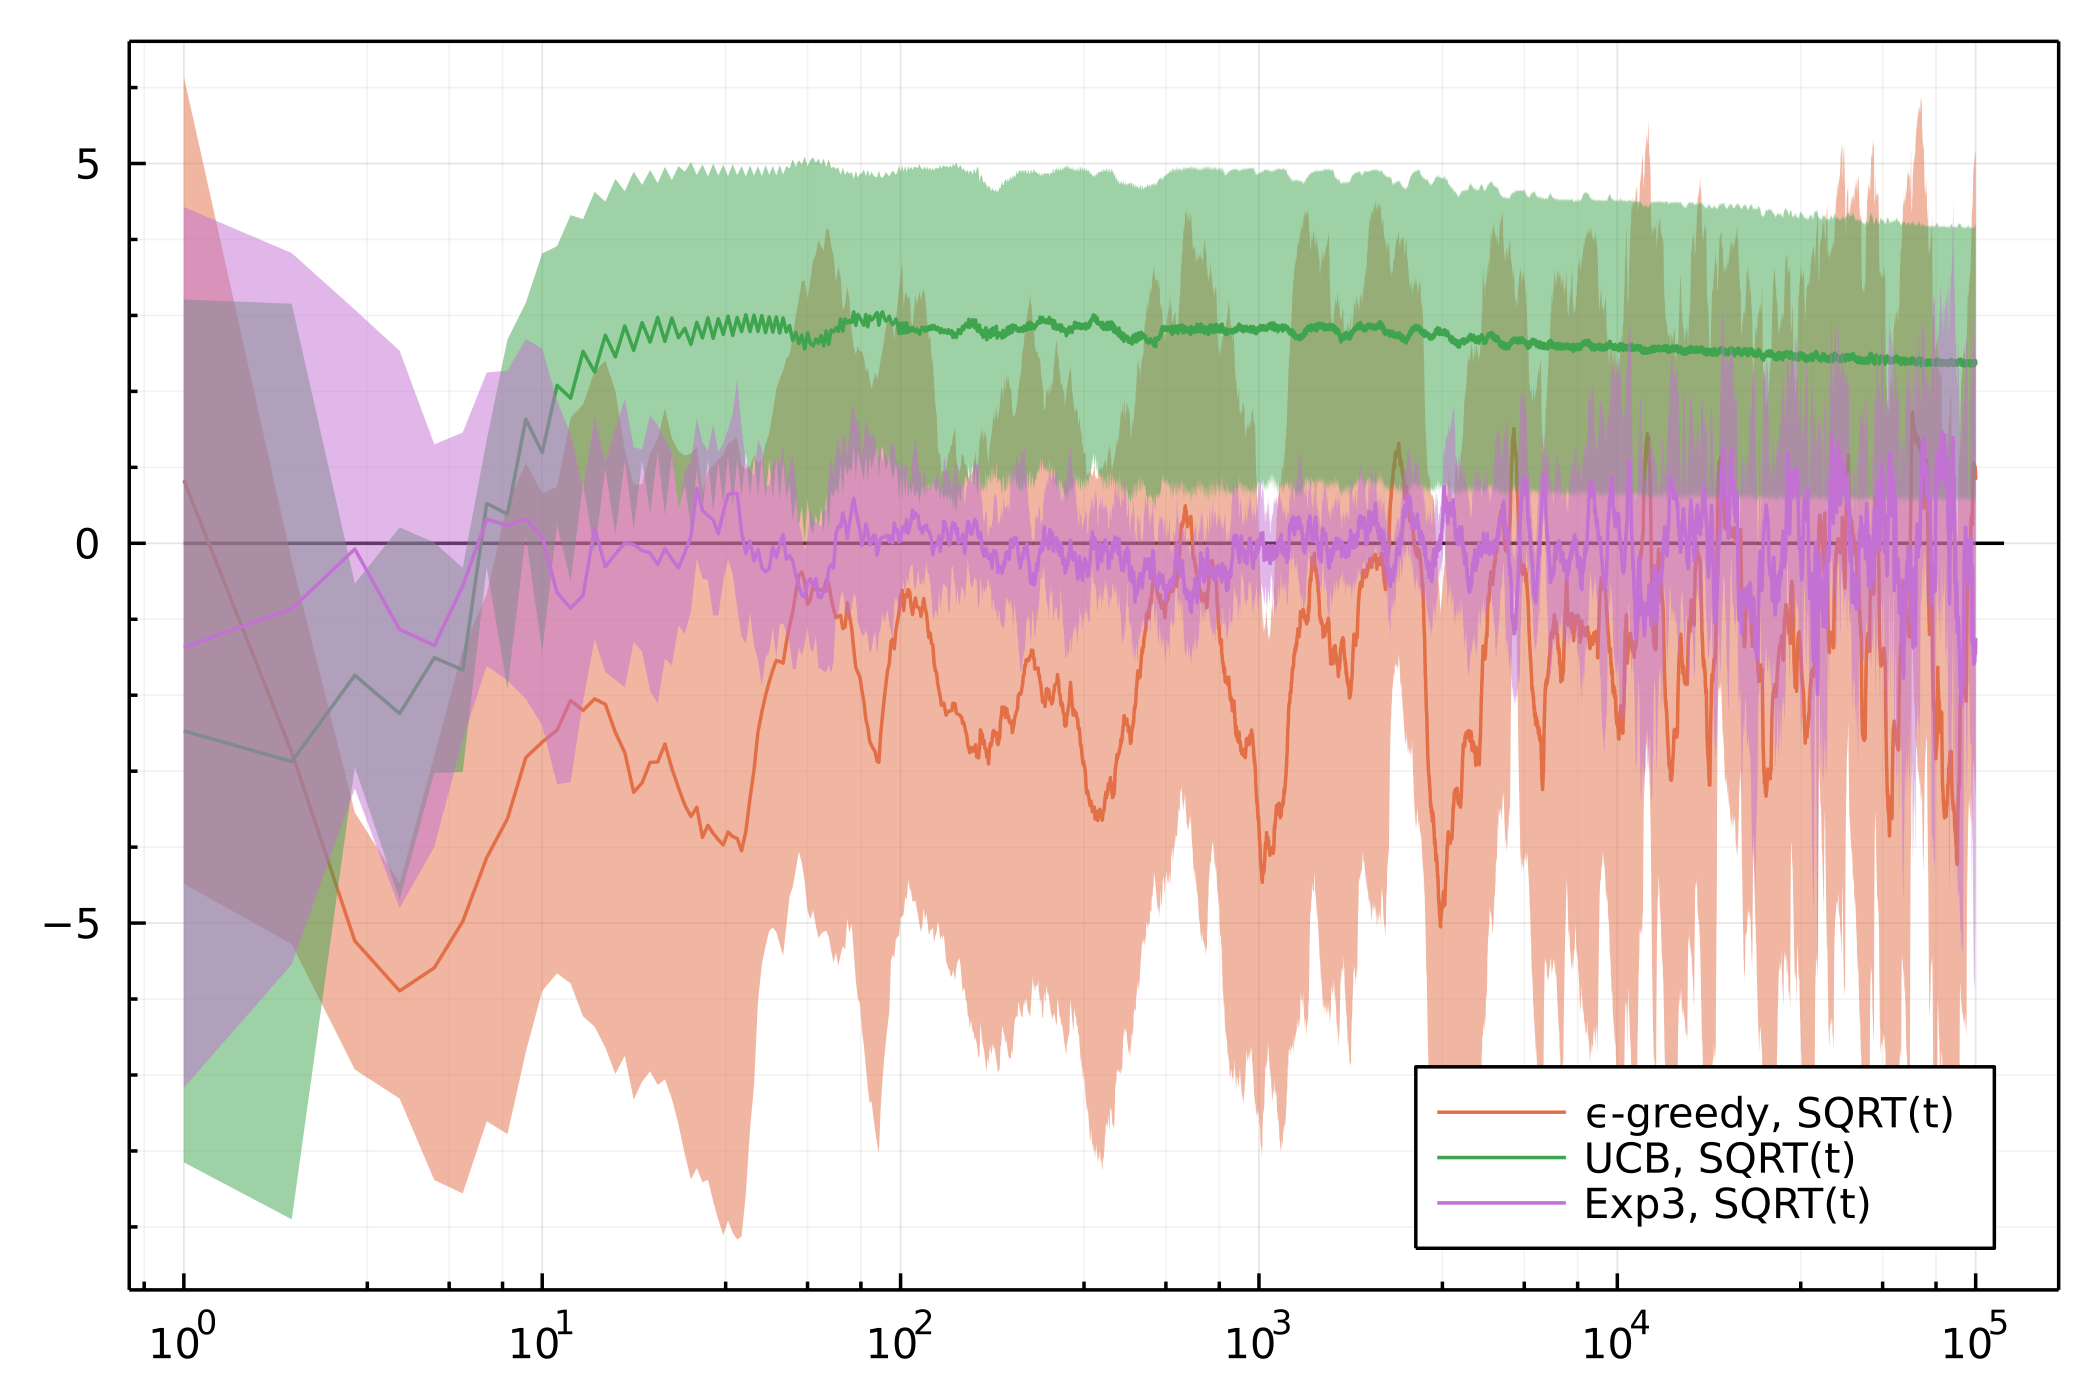
\includegraphics[width=1\textwidth]{sg/best/graphs_5_01_EpsilonGreedy_UCB_Exp3_SqrtT_3_3.png}
        \caption{Standard bandits with $\sqrtt$ step}
        \label{exp:sg:best:5:33:std:sqrt}
    \end{subfigure}
    \begin{subfigure}[t]{0.45\linewidth}
        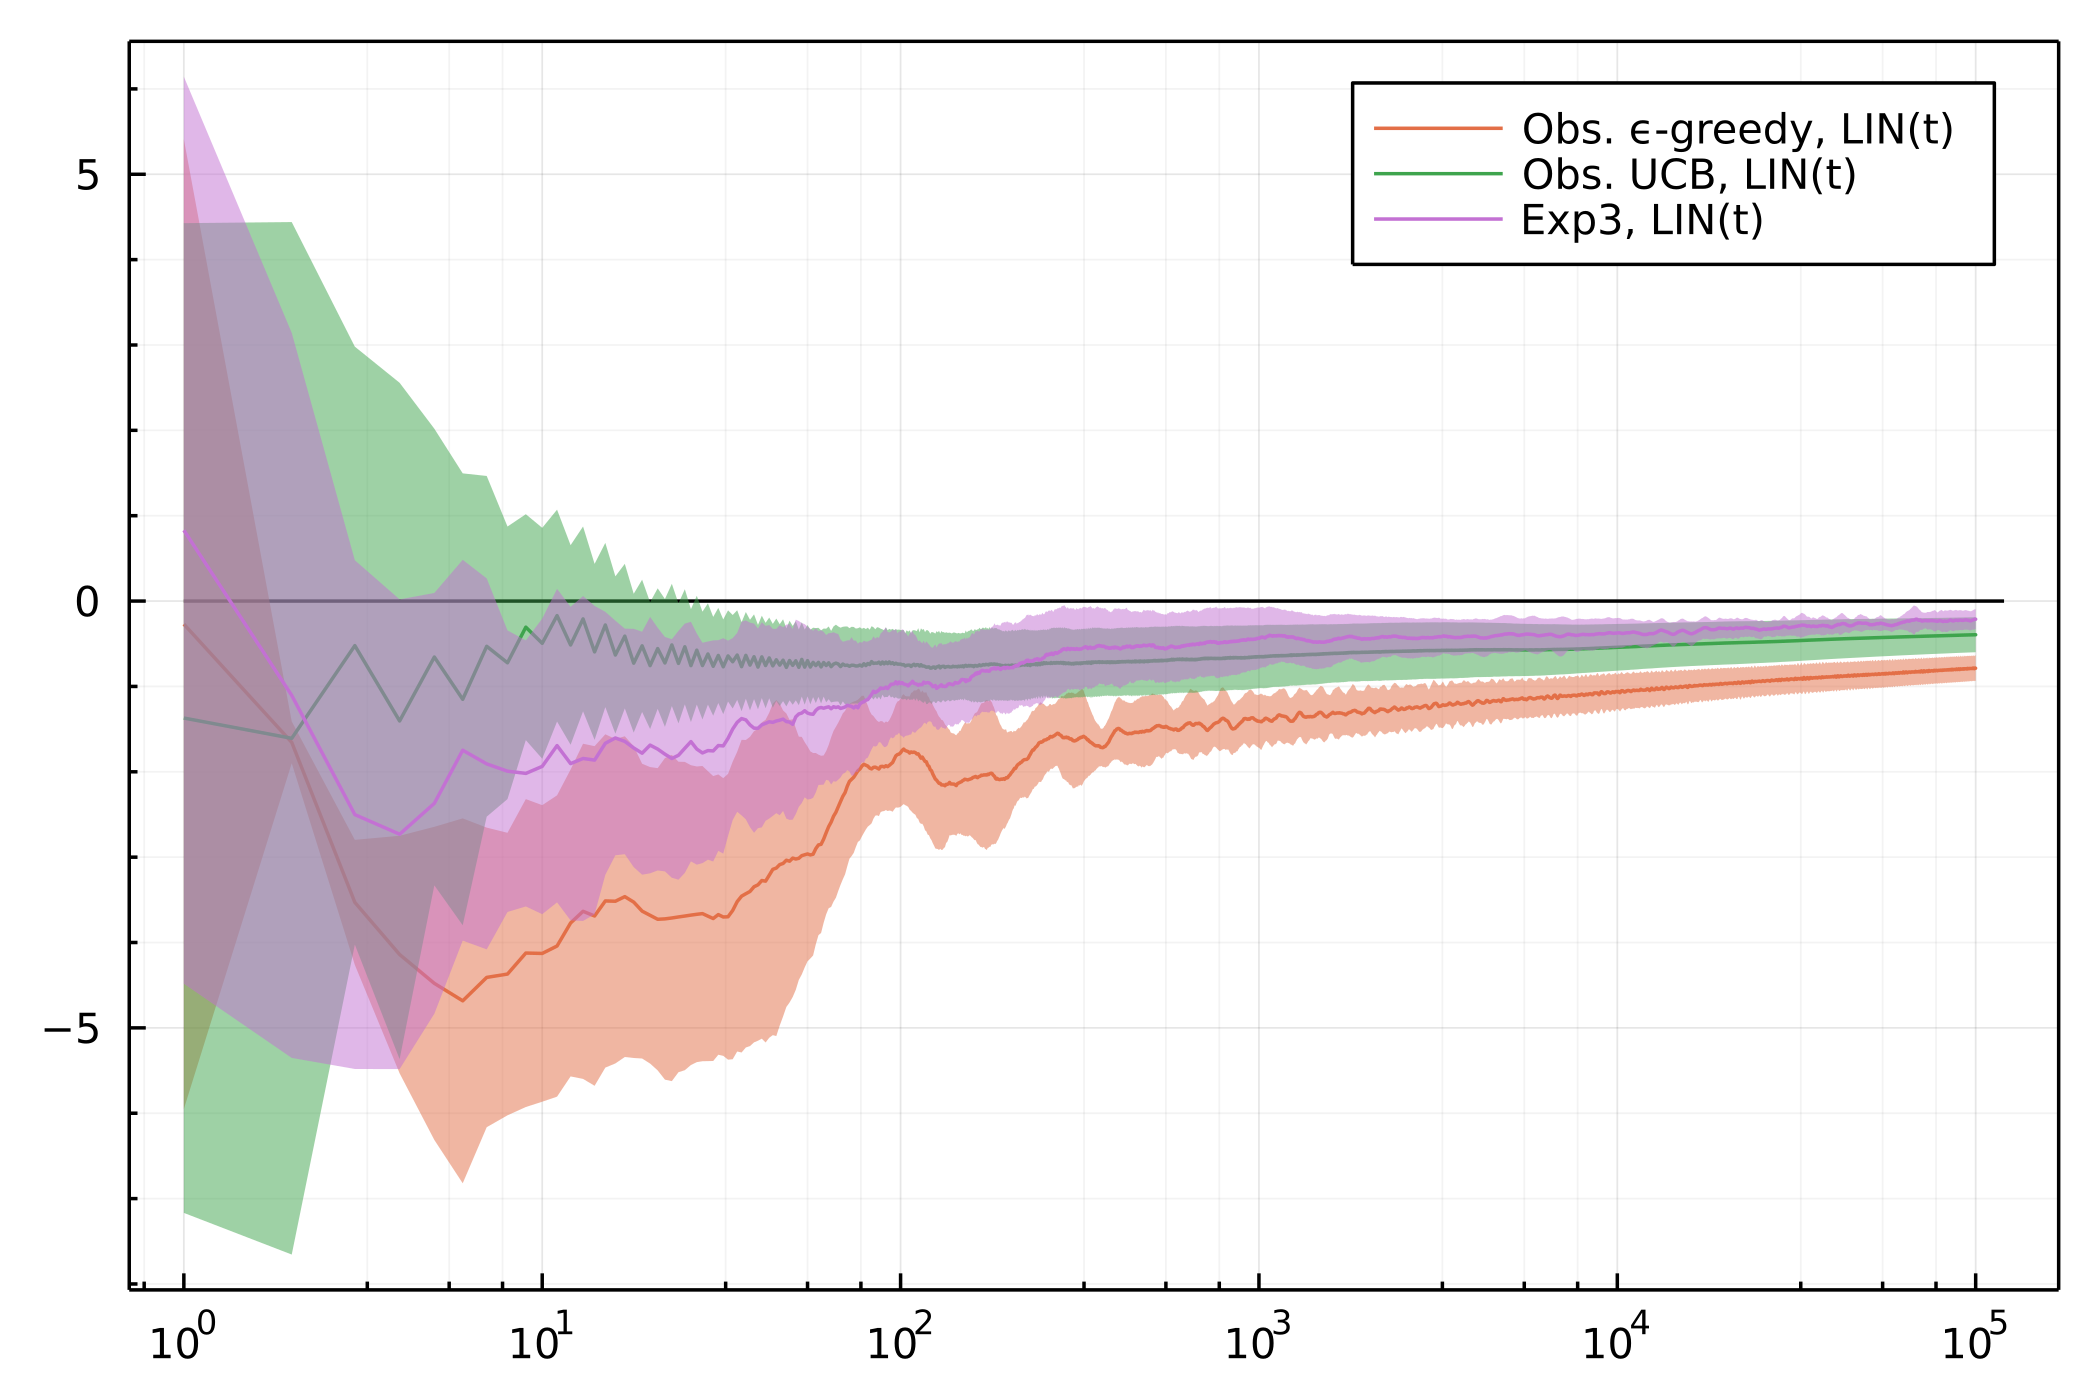
\includegraphics[width=1\textwidth]{sg/best/graphs_5_01_ObservableEpsilonGreedy_ObservableUCB_Exp3_LinT_3_3.png}
        \caption{Observable bandits with $\lint$ step}
        \label{exp:sg:best:5:33:obs:lint}
    \end{subfigure}
    \hfill
    \begin{subfigure}[t]{0.45\linewidth}
        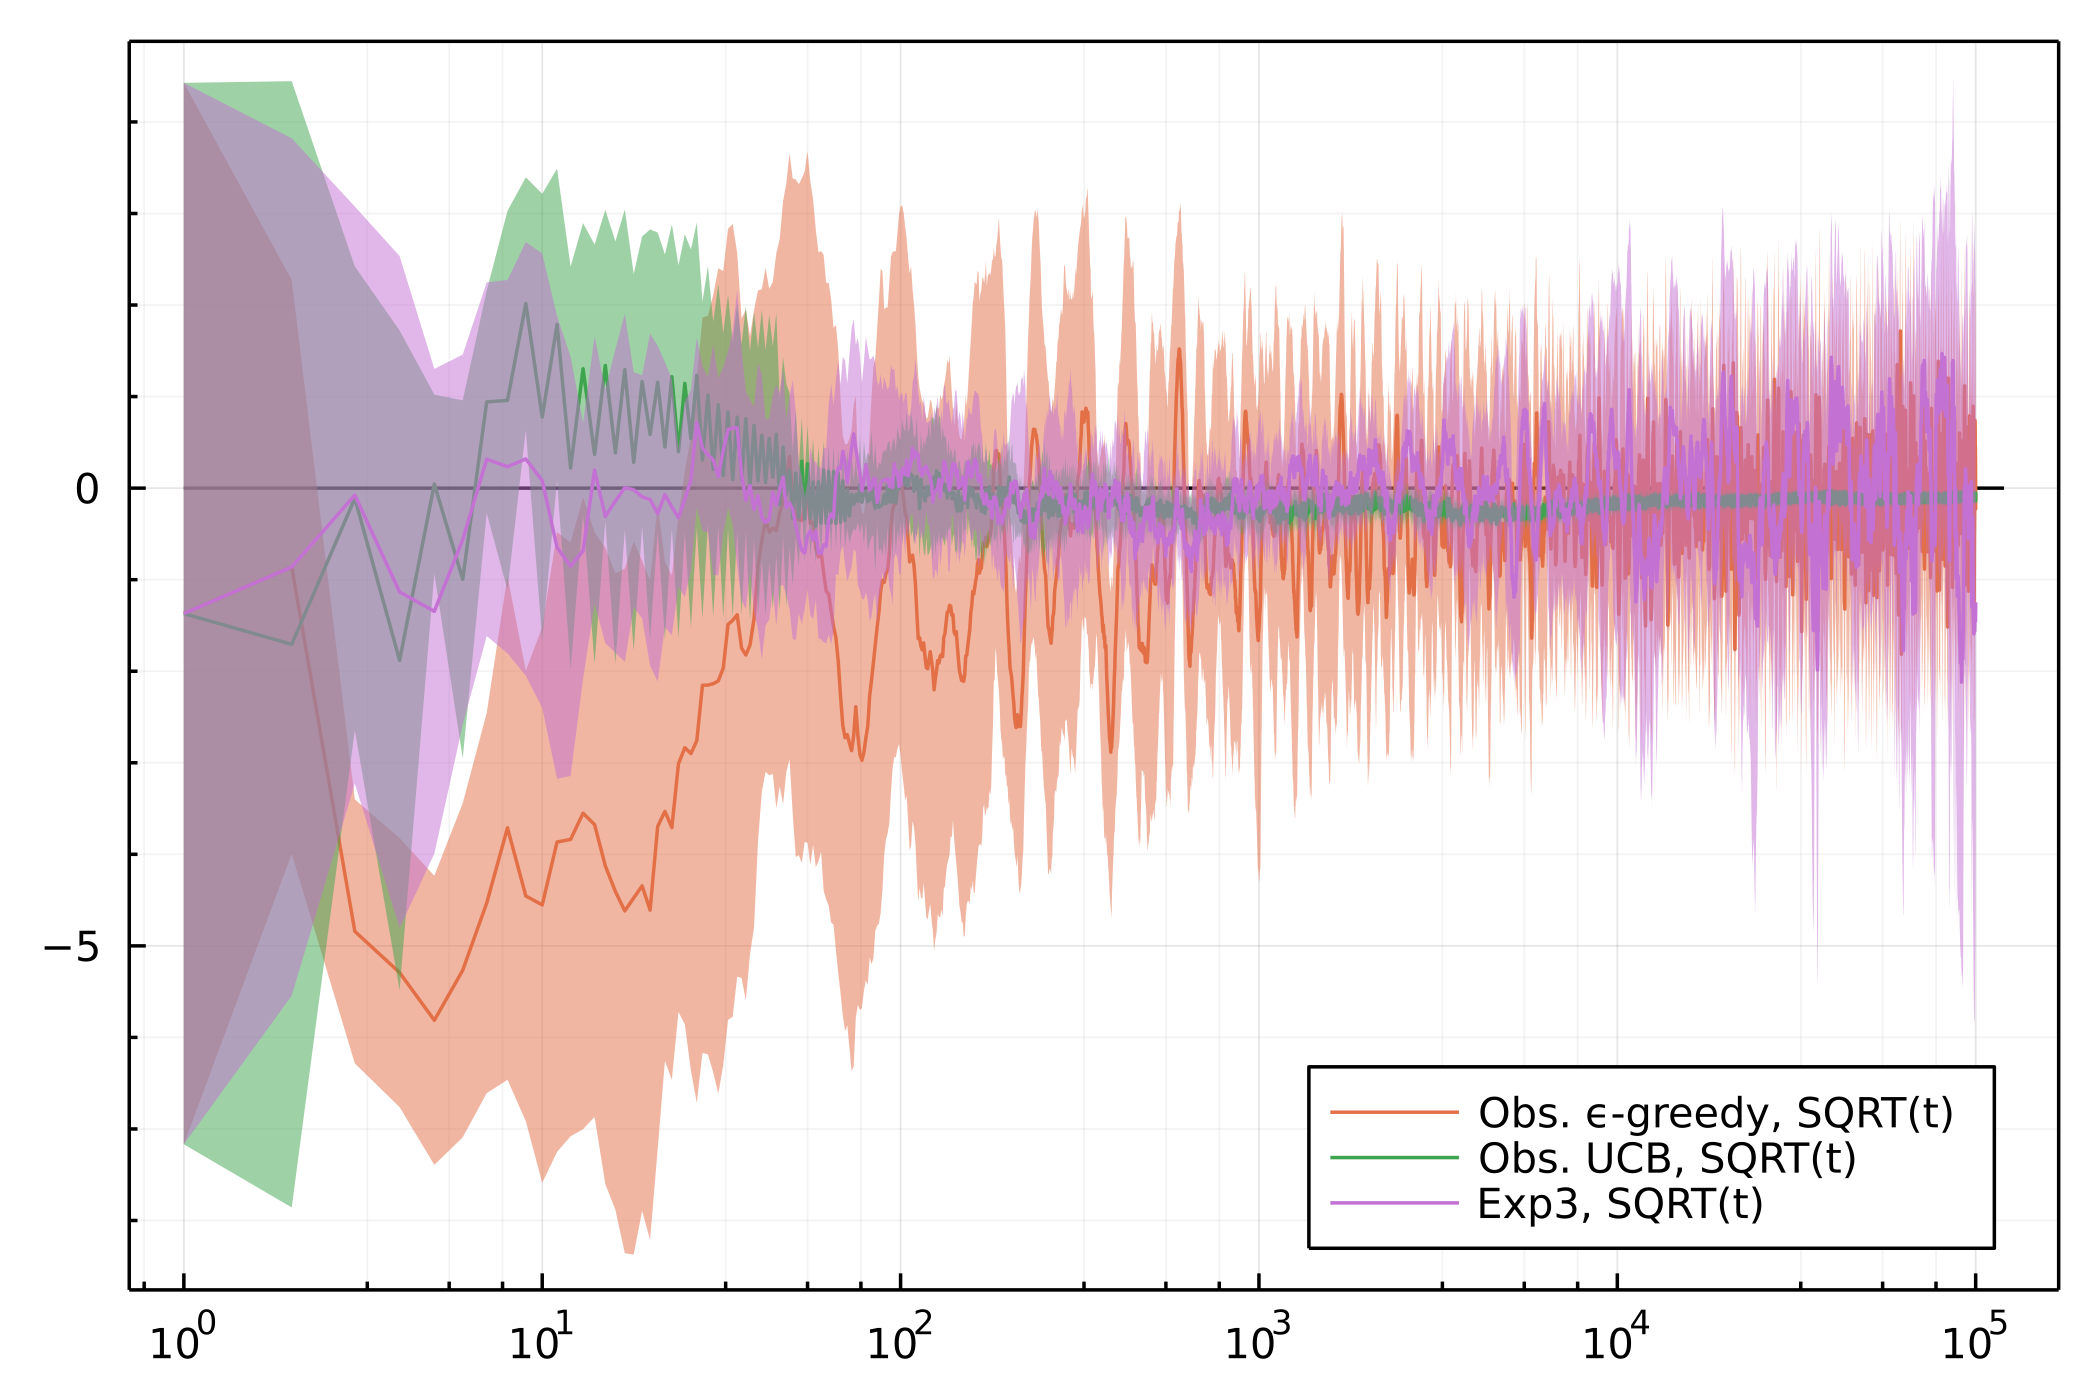
\includegraphics[width=1\textwidth]{sg/best/graphs_5_01_ObservableEpsilonGreedy_ObservableUCB_Exp3_SqrtT_3_3.png}
        \caption{Observable bandits with $\sqrtt$ step}
        \label{exp:sg:best:5:33:obs:sqrt}
    \end{subfigure}
    \caption[Comparison of three best bandits and their observable counterparts on \chasename{5} in a state $s = \left(3, 3\right)$]{
        This quartet of figures studies development of deviation of learned values from the value iteration result over time.
        The comparison is made on a \textbf{Chase} instance \chasename{5} in a mixed-strategy state $s = \left(3, 3\right)$ for the three best bandits from previous comparisons, $\epsilon$-greedy, UCB and Exp3, in combination with the two step functions, $\lint$ and $\sqrtt$.
        The top half compares the standard bandits together, the bottom half their observable complements.
    }
    \label{exp:sg:best:5:33}
\end{figure}
Here \reffig{exp:sg:best:5:33}, the situation can be divided into two categories.
First, the observable variants converge for both step function, only the $\sqrtt$ causing more oscillation at the end.
Second, the non-observable $\epsilon$-greedy approaches the optimal value but not as quickly and precisely as Exp3.
The non-observable UCB converges to another value, because it found a pure strategy in a state when mixed one is required.

\subsection{Strategies}
Here we shortly list and compare strategies acquired by the bandit algorithms in an example state.
The strategy is computed as the average use of that said arm.
In terminology from \refsec{bandit:learn} the strategy in state $s$, which is being learned by the bandit, is computed as
\begin{equation}
    \pi(a) = \frac{n^t(a)}{\sum_{a \in A}n^t(a)} \qquad \forall a \in A.
\end{equation}

In the table \reftab{exp:sg:strategies}, the average policies over the $10$ runs are listed.
For simplicity, we include only the runs with $\sqrtt$ step and only the strategies of the Tagger.
\begin{table}
    \centering
    \begin{tabular}{ l | r | r | r | r | r | r }
         & $\Updownarrow$ & $\Leftrightarrow$ & $\uparrow$ & $\rightarrow$ & $\downarrow$ & $\leftarrow$ \\
        \hhline{=|=|=|=|=|=|=}
        \rowcolor{lightgray} value iteration & 0 & 0 & 0.4 & 0.6 & 0 & 0 \\
        \hline
        Best of N & 0.997 & 0.001 & 0.001 & 0.001 & 0 & 0 \\
        Obs. Best of N & 0.997 & 0.001 & 0.001 & 0.001 & 0 & 0 \\
        \hline
        $\epsilon$-greedy & 0.07 & 0.21 & 0.18 & 0.54 & 0 & 0 \\
        Obs. $\epsilon$-greedy & 0.03 & 0.27 & 0.26 & 0.69 & 0 & 0 \\
        \hline
        Successive elim. & 0.02 & 0.02 & 0.02 & 0.94 & 0 & 0 \\
        Obs. Successive elim. & 0.02 & 0.03 & 0.02 & 0.93 & 0 & 0 \\
        \hline
        UCB & 0.01 & 0.16 & 0.21 & 0.62 & 0 & 0 \\
        Obs. UCB & 0.0 & 0.10 & 0.23 & 0.66 & 0 & 0 \\
        \hline
        Exp3 & 0.01 & 0.08 & 0.27 & 0.64 & 0 & 0
    \end{tabular}
    \caption[Tagger's strategies on \tagname{3}{01} in a state $s = \left(3, 3\right)$]{
        This table compares strategies learned by individual bandits used in the bandit iteration framework to the optimal mixed strategy found by the value iteration algorithm.
        These depicted Tagger's strategies correspond to distributions over actions: $\Updownarrow$ = "shoot beam vertically"; $\Leftrightarrow$ = "shoot beam horizontally"; $\uparrow$, $\rightarrow$, $\downarrow$, $\leftarrow$ = "move to the adjacent square determined by the direction of the arrow".
        This strategy was learned on \textbf{Tag} instance \tagname{3}{01} in a state $s = \left(3, 3\right)$.
    }
    \label{exp:sg:strategies}
\end{table}
The data in the table confirm what was already clear in the graph comparison before.
The best of N simply selects the best action after the first N trials, while successive elimination removes the not so good arms.
But both of them do not reach near the optimal strategies and thus could not converge to the optimal 0 deviation in the experiments before.

The rows for $\epsilon$-greedy show that the bandit truly explores as it has a bit bigger usage of actions $\Updownarrow$ (shoot laser beam vertically) and $\Leftrightarrow$ (shoot laser beam horizontally) which are not used in the optimal strategy at all.
Moreover, it can be said that the other bandits explore a lot less.

The UCB together with the observable variant gets quite close to the values found by the value iteration.
It should be noted, that most of these strategies could turn out better if the beginning was not included.
If the probabilities were computed from let's say second half, it could filter the wrong choices in the beginning and thus get closer to the optimal strategies.

The Exp3 bandit results in very similar average strategy as the UCB and observable UCB algorithms and thus is again close to the optimum.

\section{OS-POSGs and B-HSVI algorithm}\label{exp:osposg}
In \refsec{bg:osposg} we presented the One sided partially observable stochastic game formalism used to model scenarios, where one of the adversarial agents does not have full information about the environment state.
Then, in \refsec{standard:osposg} we showed an algorithm invented by \cite{osposgs}, which is proven to approximately solve problems modelled as OS-POSGs with the use of linear programming.
To avoid the poor scalability of such linear program, which can grow very large for partially observable settings, we altered the HSVI algorithm to form a new method called B-HSVI in \refsec{new:bhsvi}.

Here, we experimentally evaluate the B-HSVI algorithm and compare the different multi-armed bandit type selections on a selected instance of an OS-POSG game.
In contrast to the SGs, the observable variants cannot be applied to this setting.
Therefore, we consider only the standard bandit algorithms receiving feedback only for actions selected by them.

Note, that we will focus mainly on the results which are different from the previous comparisons
The similarities will be mentioned but not thoroughly analysed.

\subsection{Pursuit-Evasion}\label{exp:osposg:type}
For comparison purposes we selected a game type similar to the \textit{Chase} and \textit{Tag} game types called \textit{Pursuit-evasion}, or shortly \textbf{PEG}.
This game type is taken from \cite{poposgsthesis} and was inspired by \cite{peg1}.

The game is played on a grid with a fixed number of rows and instance-dependent number of columns.
The two players are then placed in the environment and their actions correspond to moving to an adjacent square.
The player 1, called the \textit{Pursuer} and represented by $n$ independent units, aims to get one of these units on the same grid cell as the \textit{Evader}'s single unit and this way terminate the game.
The Evader, on the other hand tries to escape for as long as possible.
For catching the Evader, the Pursuer receives reward $1.0$, otherwise $0.0$.

As player 1, the Pursuer does not have full information, thus the position of the Evader is unknown to him.
To simplify the problem, we employ the information sets \refother{standard:osposg:infoset}, hence allowing the Pursuer to know perfectly his own positions on the grid, effectively reducing the dimension of the belief search space.
The Evader has access to full information and knows his and the adversary's states and the actions played by both of them.

For the comparison purposes, we set the parameters of the game to a grid $3 \times 3$ and fix the number of Pursuer unit to $n = 2$.
However, for the sake of clarity, the transition probabilities are either $1$ or $0$, thus prohibiting failed effects of actions.

For the comparisons, we consider two initial settings as shown on \reffig{exp:osposg:type:fig}.
The setup on the right should be a bit easier for the algorithm to solve as the Evader is with some probability very close to getting caught.

\begin{figure}[ht]
    \centering
    \begin{subfigure}[b]{0.45\textwidth}
        \centering
        \begin{tikzpicture}
            \foreach \x in {0,1,2}{\foreach \y in {0,1,2}\node[box] at (\x,\y){};}
            \node[box] at (0, 2) {\Large$\bullet$};
            \node[box] at (1, 2) {\Large$\bullet$};
            \node[box] at (2, 2) {};

            \node[box] at (0, 1) {};
            \node[box] at (1, 1) {};
            \node[box] at (2, 1) {};

            \node[box] at (0, 0) {};
            \node[box] at (1, 0) {};
            \node[box] at (2, 0) {1.0};
        \end{tikzpicture}
        \caption{\textbf{PEG 1} with initial belief $\binit_1$}
        \label{exp:osposg:type:fig:1}
    \end{subfigure}
    \hfill
    \begin{subfigure}[b]{0.45\textwidth}
        \centering
        \begin{tikzpicture}
            \foreach \x in {0,1,2}{\foreach \y in {0,1,2}\node[box] at (\x,\y){};}
            \node[box] at (0, 2) {0.25};
            \node[box] at (1, 2) {\Large$\bullet$};
            \node[box] at (2, 2) {0.25};

            \node[box] at (0, 1) {};
            \node[box] at (1, 1) {\Large$\bullet$};
            \node[box] at (2, 1) {};

            \node[box] at (0, 0) {0.25};
            \node[box] at (1, 0) {};
            \node[box] at (2, 0) {0.25};
        \end{tikzpicture}
        \caption{\textbf{PEG 2} with initial belief $\binit_2$}
        \label{exp:osposg:type:fig:2}
    \end{subfigure}
    \caption[Example \textbf{PEG} instance]{
        Illustration of the environment, where the game of \textbf{PEG} \refsec{exp:osposg:type} is played.
        In the figures, the $\bullet$ symbol represents the units of the Pursuer and the numbers, represent the initial belief $\binit$ about the position of the Evader.
    }
    \label{exp:osposg:type:fig}
\end{figure}

\subsection{Environment and parameters}\label{exp:osposg:env}
As in the previous comparison, the convergence of the individual bandit algorithms inside the B-HSVI algorithms depends on the parameters and the means of evaluation.
These details are briefly described in this section.

\subsubsection{Reference}\label{exp:osposg:env:ref}
As well as in the previous experiments, we need some referential solution to which all the bandit algorithms will be compared.
Ideally, we would take the exact optimal solution, but for this class of problems, this value is not available.
Thus, we use the result of the original HSVI algorithm, which is proven to converge to an $\epsilon$-neighbourhood of the true solution.

Specifically, we solved the two possible initial settings of the \textbf{PEG} game instance \reffig{exp:osposg:type:fig} to a precision $\epsilon = 10^{-4}$.
The retrieved solution is a tuple $\left(l, u\right)$ where $l \in \mathbb{R}$ is the lower bound and $u \in \mathbb{R}$ is the upper bound and where $l \leq u$.
The value used as a reference then corresponds to the number exactly between these two bounds, i.e. the arithmetic average of $l$ and $u$.

In the experiments we observe how the bandits and the B-HSVI approach this referential value.

\subsubsection{Means of evaluation}\label{exp:osposg:env:eval}
As opposed to the value iteration and bandit iteration for stochastic games, the HSVI-based algorithms only focus on finding the close approximation of the initial state and the value of the others is not guaranteed to be inside the $\epsilon$-neighbourhood.
To provide two different situations for comparison we choose the two initial starting settings as described in \refsec{exp:osposg:type}.
On the other hand, with these bounds-focused algorithms there are two possible means of comparison of the individual runs, each convenient for different type of analysis.
The first is tracking the approach of the two bounds to the optimal value somewhere between them.
We focus on this to better distinguish between behaviour of the bandits on the lower bound and the upper bound.
The second and least important one is observing the gap between the two bounds going to zero, which provides a more general idea about the convergence of the algorithm.

\subsubsection{Setting}\label{exp:osposg:env:runs}
Experiments were conducted on the \textbf{PEG} instance described in \refsec{exp:osposg:type} on both initial starting points as shown in \reffig{exp:osposg:type:fig}.
Moreover, each run was repeated both with the default discount factor $\gamma = 0.95$ and with a smaller one $\gamma = 0.9$.

Each of these types of problems were executed $5$ times for each non-observable bandit algorithm with multiple different parameter values.
The runs were set up for $5 \cdot 10^4$ discrete time steps, where one time step corresponds to a single update of both the lower and upper bound.
This number of time steps corresponds to approximately 8-10 hours of solve time on the \textit{Metacentrum} machine mentioned at the beginning of the chapter.
All the runs had a unique random seed for the pseudo-random number generator.

The parameters selected for comparisons were decided by similar rules of thumb as in the previous experiments.
The best found values for individual algorithms are compared later in this chapter in \refsec{exp:osposg:individual}.

\subsubsection{Graphs}\label{exp:osposg:env:graphs}
As in the experiments for stochastic games, the analysis includes demonstration on the graphs, even though, there are a few differences from the previous ones.
Similarly, the $y$ axis corresponds to a mean value over the $5$ runs highlighted in full colour with the band of standard deviation around it.
However, here the number of evaluations is not as big and the graphs are synoptic so there is no need for logarithmic scale on the $x$ axis.
For more technical details see \refsec{exp:sg:env:graphs}.

The least important type of graphs is the plot displaying convergence of the gap between bounding functions to zero.
These graphs are very similar as those in \refsec{exp:sg}.

The second and more important graph type depicts how both bounds approach to the optimal value found by HSVI with linear programs.
These graphs differ as two lines highlighted by the same colour belong to a single specific bandit algorithm with given parameter value.
These are more descriptive of the course of optimization because they distinguish between the improvements in each respective bound and thus a deeper analysis can be made.

\subsection{Individual bandits}\label{exp:osposg:individual}
In this short section we discuss the bandit algorithms individually with respect to the evaluated parameters.
The interesting realizations are demonstrated on images, while the less important ones are only mentioned.

Surprisingly, most of the bandits do not change their behaviour much based on the tested parameters even though chosen really different.
The Exp3 bandit algorithm, for example, for all the selections of the explorative parameter $\gamma \in \left\{0.1, 0.25, 0.5, 1.0\right\}$ behaved almost exactly the same for all the chosen runs with only slight changes within the standard deviation interval.
The same thing can be said about the Best of N and even about the Successive elimination bandit for its exploration parameter $\alpha \in \left\{1, 2, 10\right\}$.
Thus, the parameters for the bulk comparison of the bandit algorithms were chosen as those with the best mean value even though it was never out of the interval of standard deviations of the other runs.

Conversely, the very important realization is that the UCB multi-armed bandit is not suitable for the HSVI algorithm at all.
While it and its observable complement dominated all other bandits on most instances, here it is one of the poorly performing bandits with only the Successive elimination being incomparably worse.
And it seems that the parameter which controls tightening of the confidence bounds around average reward, set similarly as for the Successive elimination, $\alpha \in \left\{1, 2, 10\right\}$ has the opposite effect than the intuitive idea.
\begin{figure}[ht]
    \begin{subfigure}[b]{0.45\textwidth}
        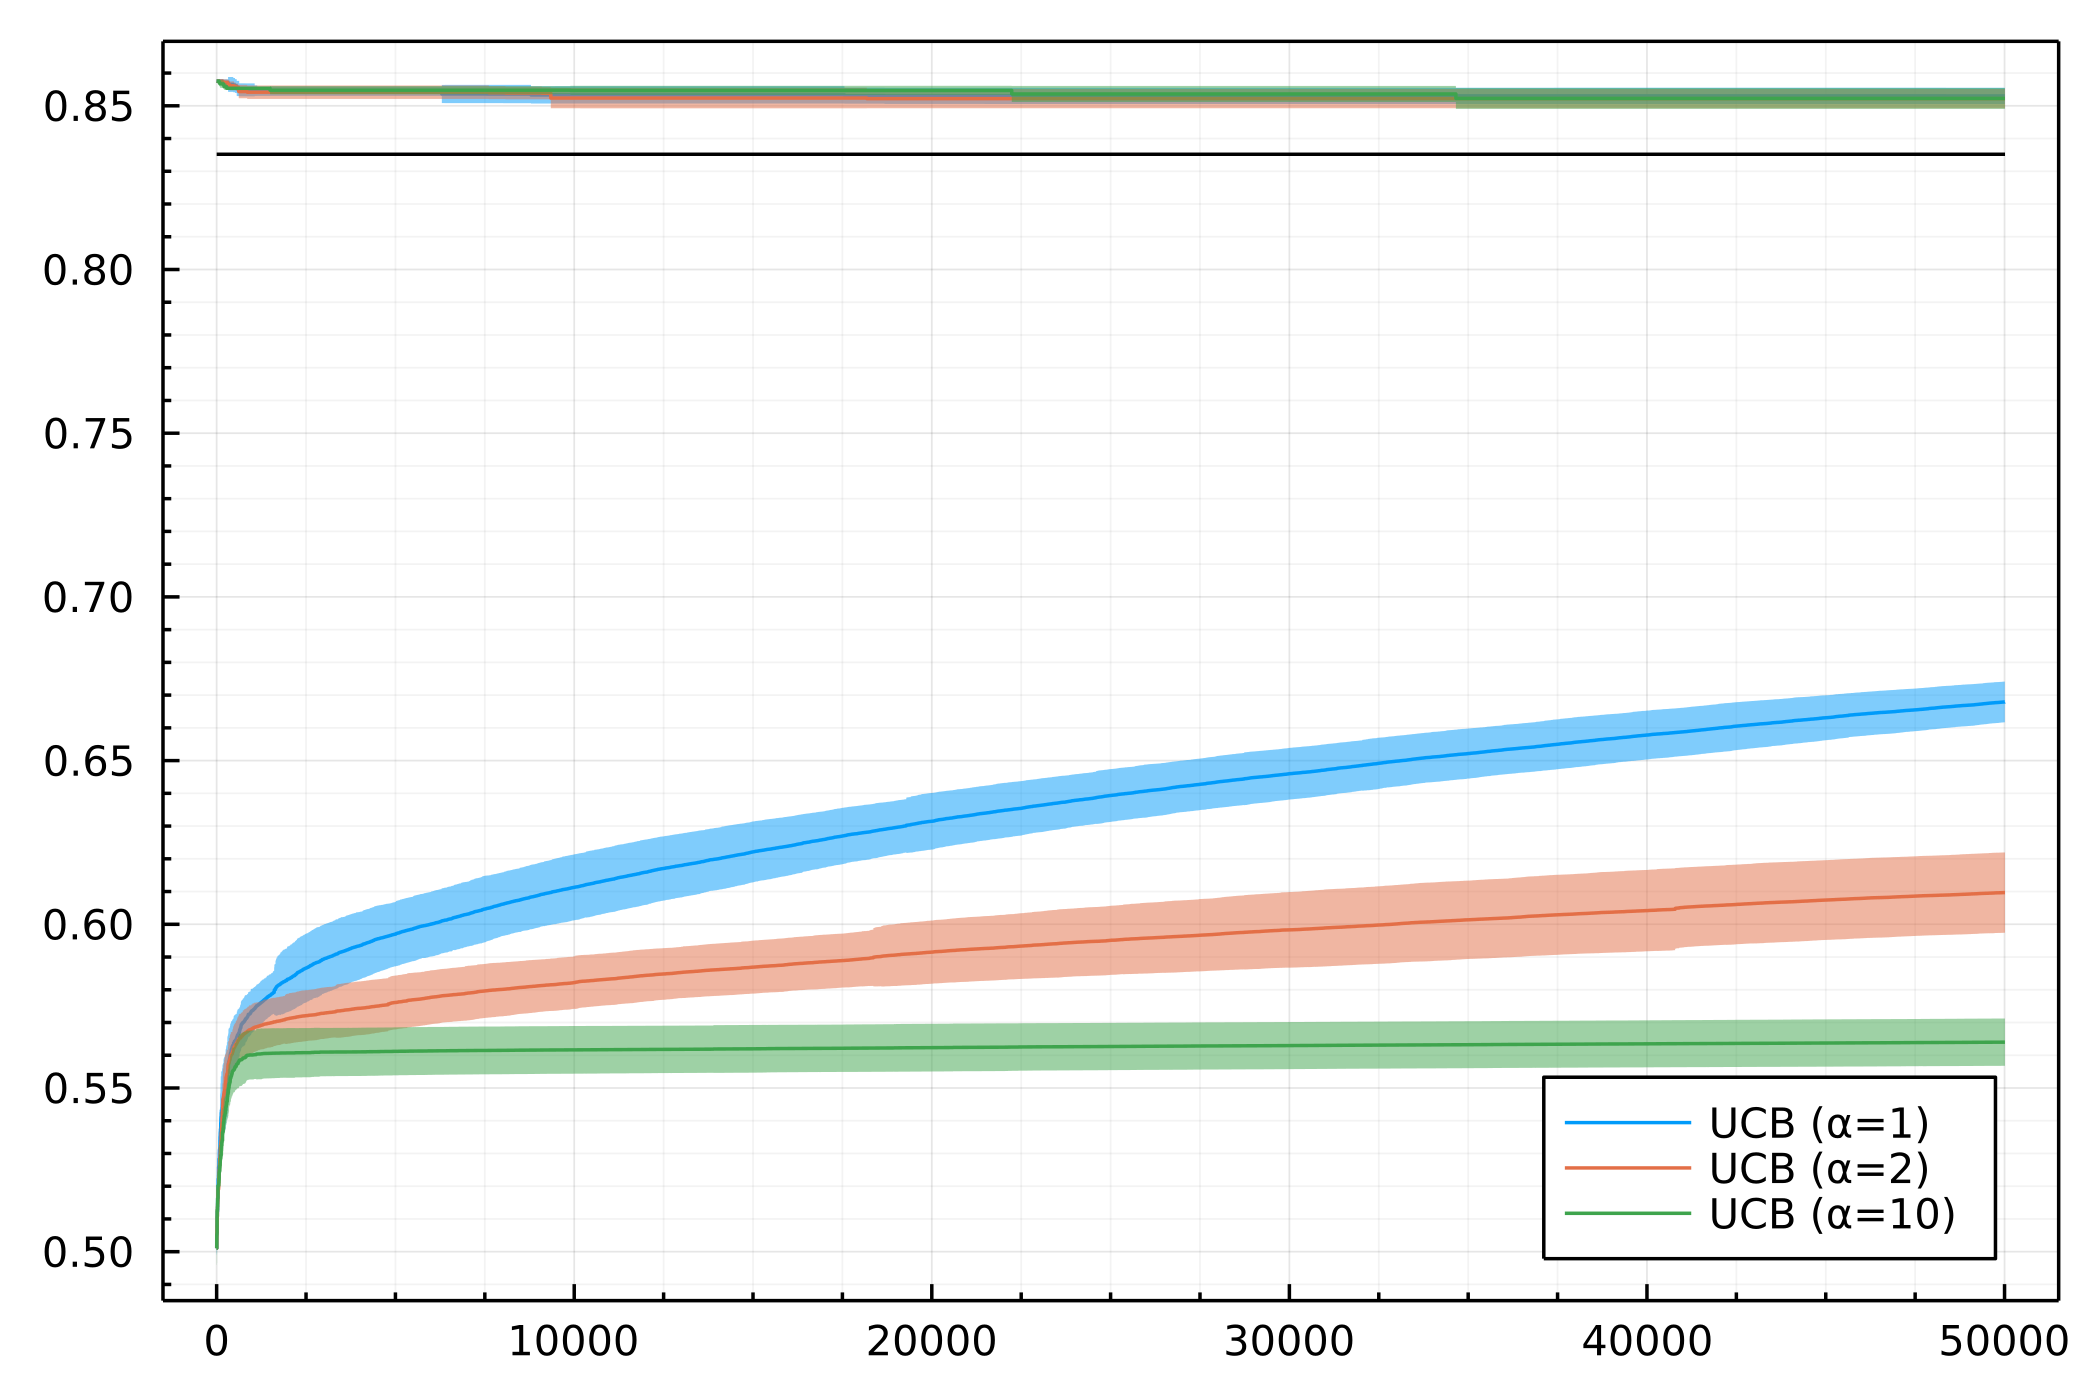
\includegraphics[width=1\textwidth]{osposg/ucb/UCB_original_discount_095.png}
        \caption{The bounds of HSVI approaching the true value}
        \label{exp:osposg:individual:ucb:bounds}
    \end{subfigure}
    \begin{subfigure}[b]{0.45\textwidth}
        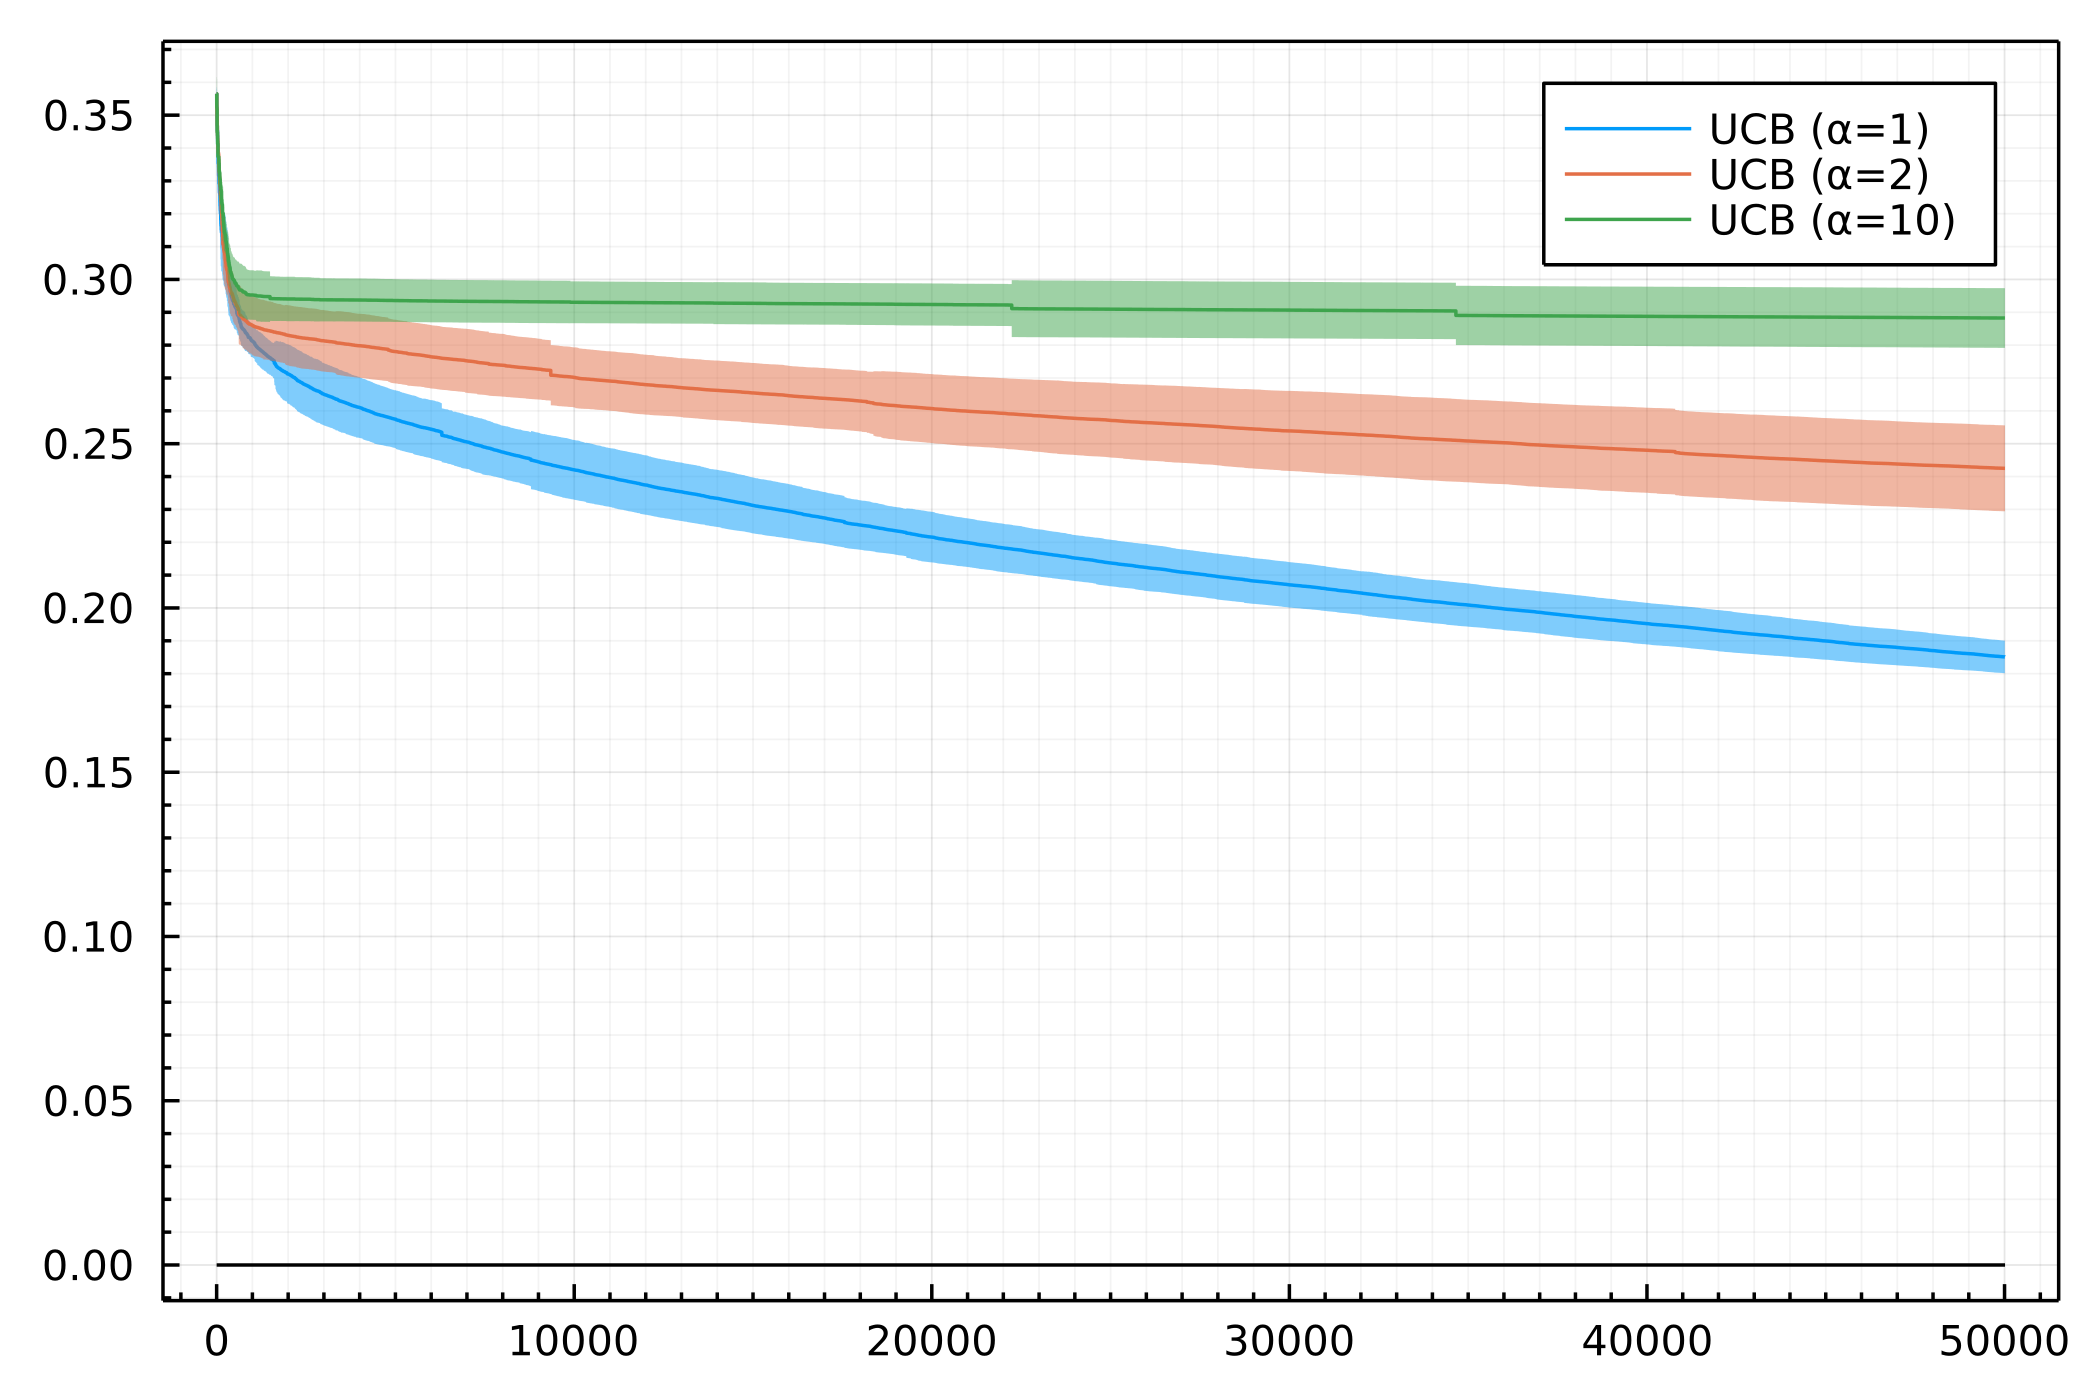
\includegraphics[width=1\textwidth]{osposg/ucb/gap_UCB_original_discount_095.png}
        \caption{The gap between bounds converging to zero}
        \label{exp:osposg:individual:ucb:gap}
    \end{subfigure}
    \caption[UCB bandit with different parameter values]{
        The behaviour of the UCB bandit algorithm on the \textbf{PEG} instance with initial settings as in \ref{exp:osposg:type:fig:1} with the discount factor $\gamma = 0.95$.
        On the left figure is show dependence of values found by the upper and lower bound on the discrete time steps representing one point-based update and how the bounds approach the true value.
        The right graph depicts convergence of the gap between bounds to zero depending on the same discrete time steps.
    }
    \label{exp:osposg:individual:ucb}
\end{figure}
The parameter setting $\alpha = 1$ shows the best results while the $\alpha = 10$ does not converge almost at all when considering the lower bound.
This goes against the conclusions from the previous experiments, where bigger exploration meant much better convergence.
It could be caused by the fact that with smaller $\alpha$ the UCB gradually degrades to the greedy bandit and as will be shown in the next comparison the $\epsilon$-greedy works well with the HSVI algorithm.

On the upper bound, the different parameters for the UCB do not show significant differences in convergence.

The best parameter over the all trials for $\epsilon$-greedy bandit algorithm is $\epsilon = 0.3$, even though not by a large margin.
This holds mainly for the lower bound, because in the upper bound the more aggressive exploration parameter value $\epsilon = 0.5$ converges slightly closer to the real value.
However, when compared by the convergence of the gap to zero, the lower bound improvements outweigh the upper bound, thus making the $\epsilon = 0.3$ a better choice overall.

With these best parameters selected, we can compare all the bandit algorithms together.

\subsection{Bulk comparison}\label{exp:osposg:bulk}
The table \reftab{exp:osposg:bulk:params} lists the parameters deemed best from the previous analysis in \refsec{exp:osposg:individual}.
These parameters are used for the comparison of all bandit algorithms together in this section.
\begin{table}
    \begin{tabular}{l || c | c | c | c | c}
        bandit & Best of N & $\epsilon$-greedy & Successive elimination & UCB & Exp3 \\
        \hline
        parameter & $N = 100$ & $\epsilon = 0.3$ & \multicolumn{2}{c |}{$\alpha = 1$} & $\gamma = 0.1$
    \end{tabular}
    \caption[Selected parameters for multi-armed bandits for the B-HSVI algorithm]{
        The best found parameter values for each individual bandit algorithm tested on \textbf{PEG} OS-POSG within the B-HSVI framework.
        The argumentation about these values is presented in \refsec{exp:osposg:individual}.
    }
    \label{exp:osposg:bulk:params}
\end{table}

The change of learning rate slightly changes the optimal solution found by the linear programming utilizing HSVI algorithm.
It would be expected, that solving the game with the lower discount factor $\gamma = 0.9$, the game would become easier for the approximate algorithms to solve.
However, during testing of the B-HSVI algorithm, it converged slightly farther from the optimal value than when the default $\gamma = 0.95$ was employed.
On the other hand, the standard deviation intervals surrounding the plotted means are noticeably tighter for the smaller discount factor than for the default one and thus the values were learned by the bandits with higher confidence.

All the bandits evaluated on the \textbf{PEG} instance with both initial settings and with the discount factor $0.95$ is shown in the \reffig{exp:osposg:bulk:fig}.
\begin{figure}[ht]
    \begin{subfigure}[t]{0.45\linewidth}
        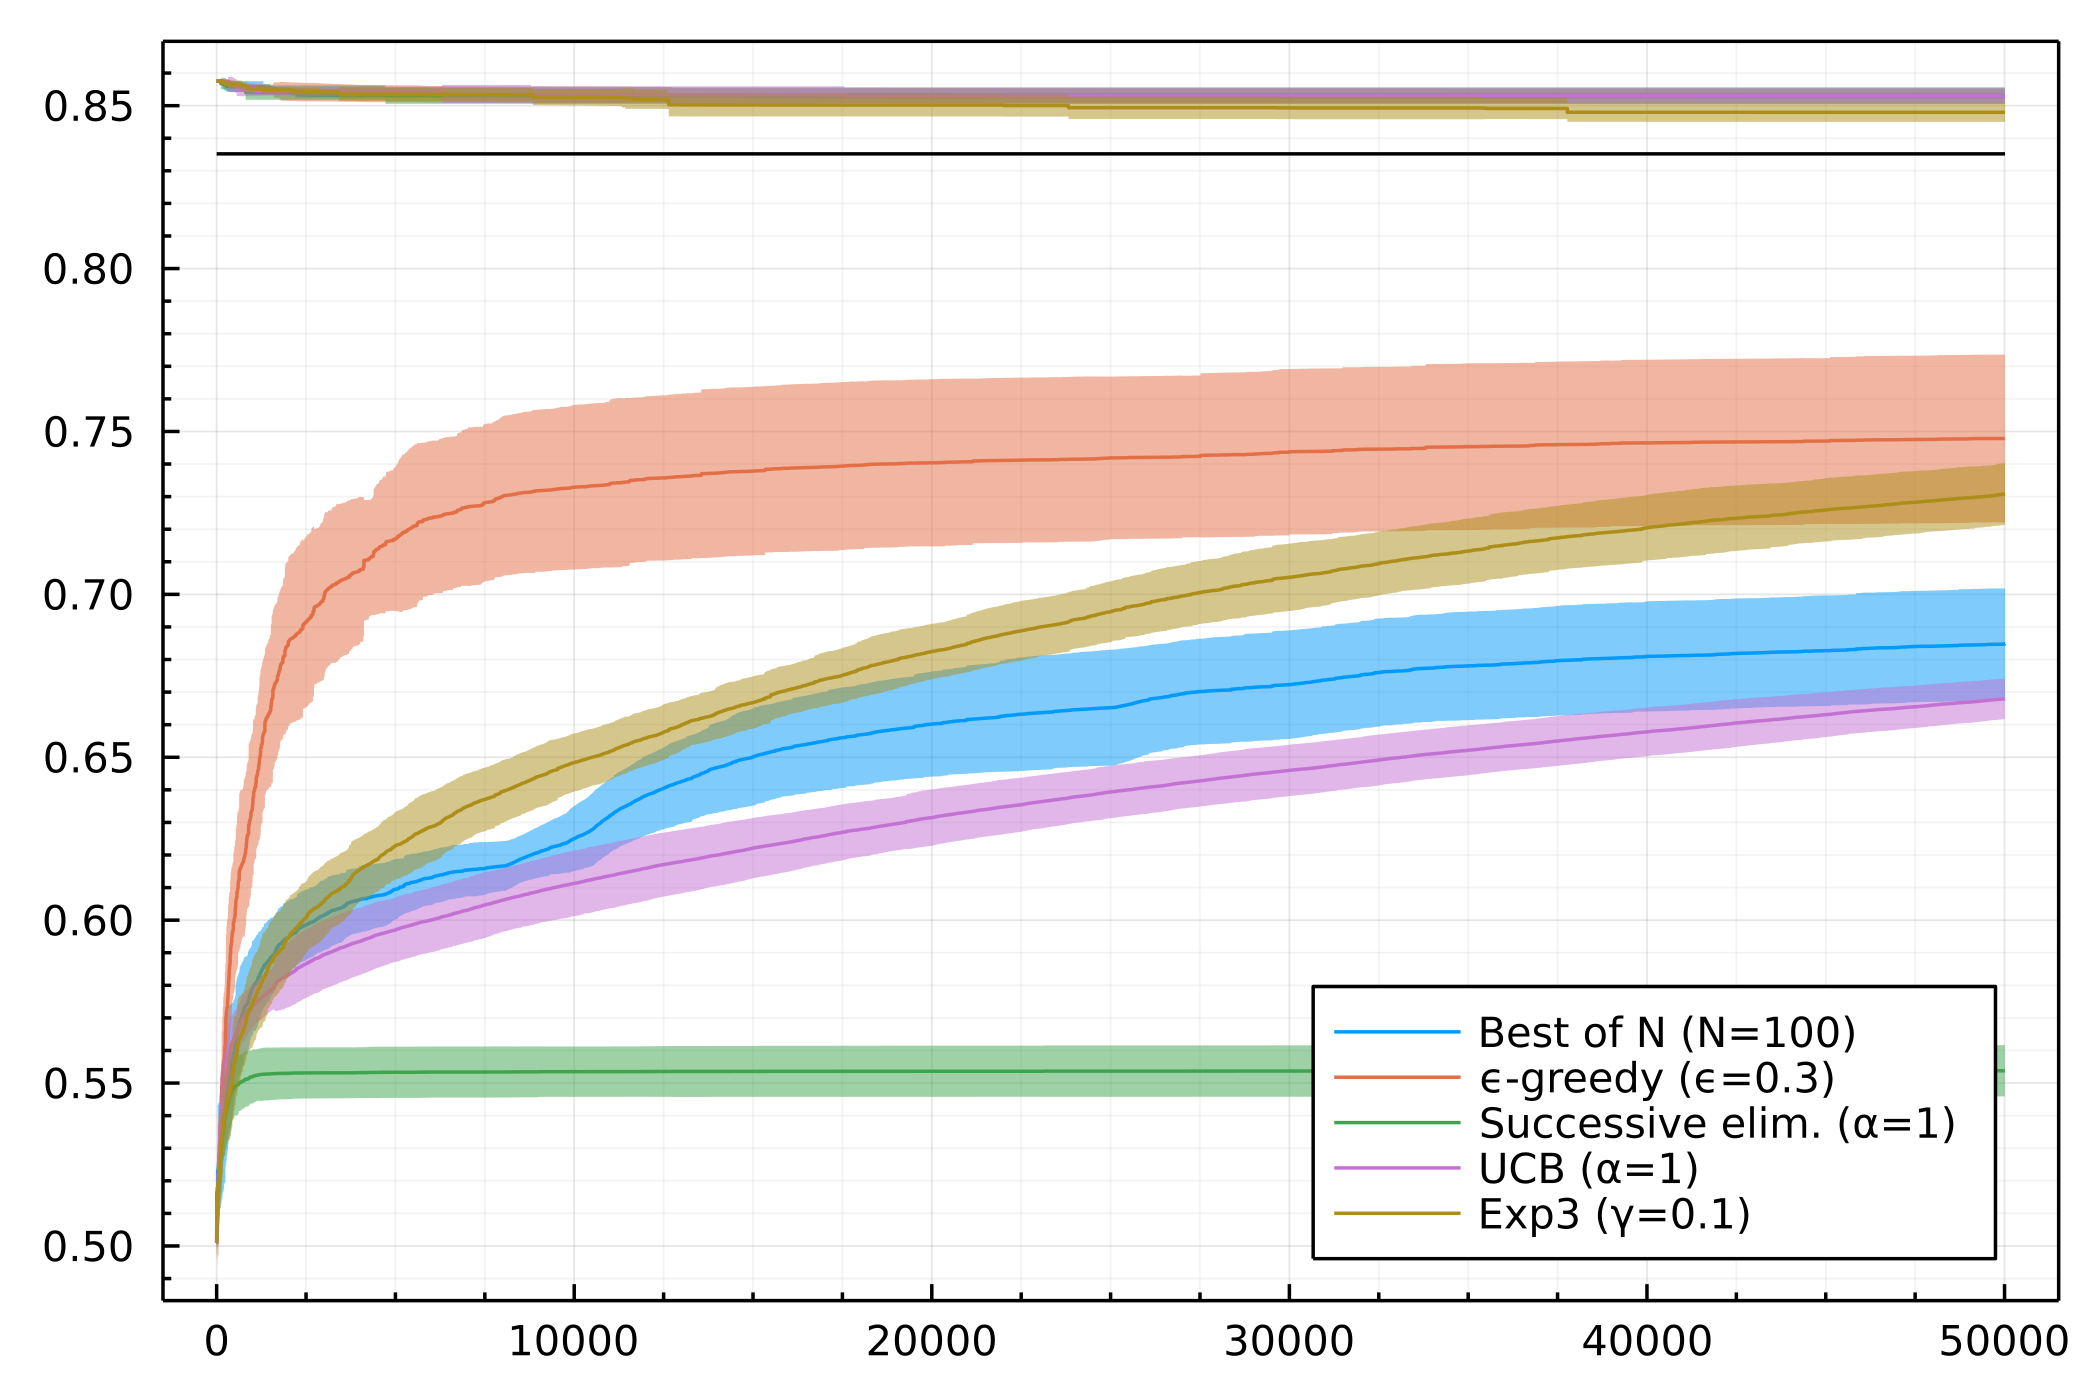
\includegraphics[width=1\textwidth]{osposg/bulk/original_discount_095.png}
        \caption{Value bounds for the original setting \reffig{exp:osposg:type:fig:1}}
        \label{exp:osposg:bulk:fig:original:bounds}
    \end{subfigure}
    \hfill
    \begin{subfigure}[t]{0.45\linewidth}
        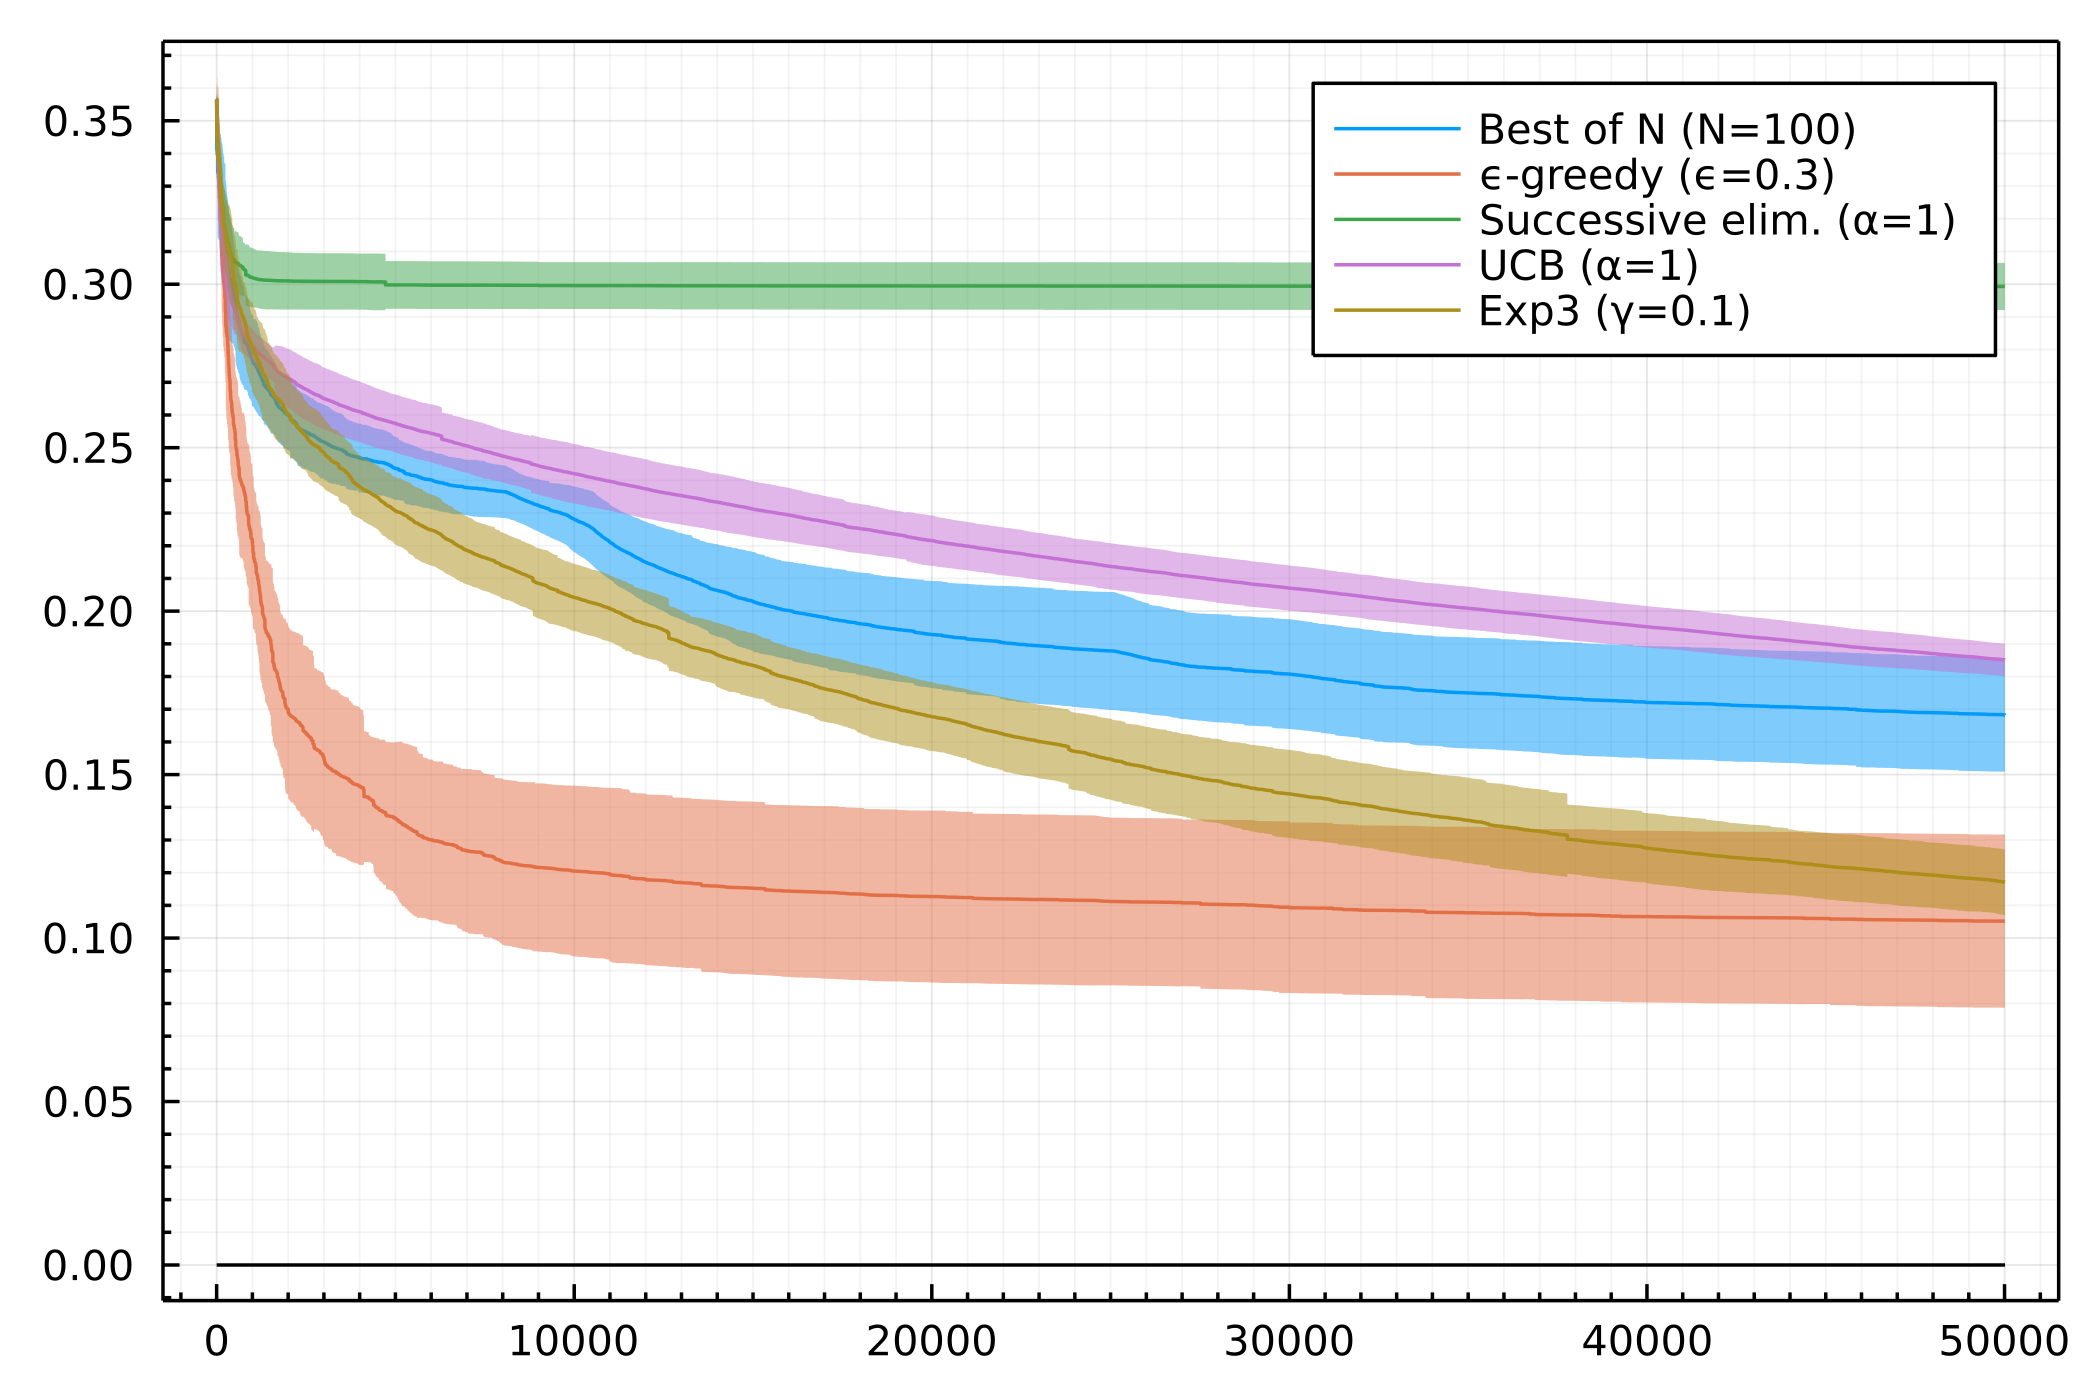
\includegraphics[width=1\textwidth]{osposg/bulk/gap_original_discount_095.png}
        \caption{Gap between the bounds for the original setting \reffig{exp:osposg:type:fig:1}}
        \label{exp:osposg:bulk:fig:original:gap}
    \end{subfigure}
    \begin{subfigure}[t]{0.45\linewidth}
        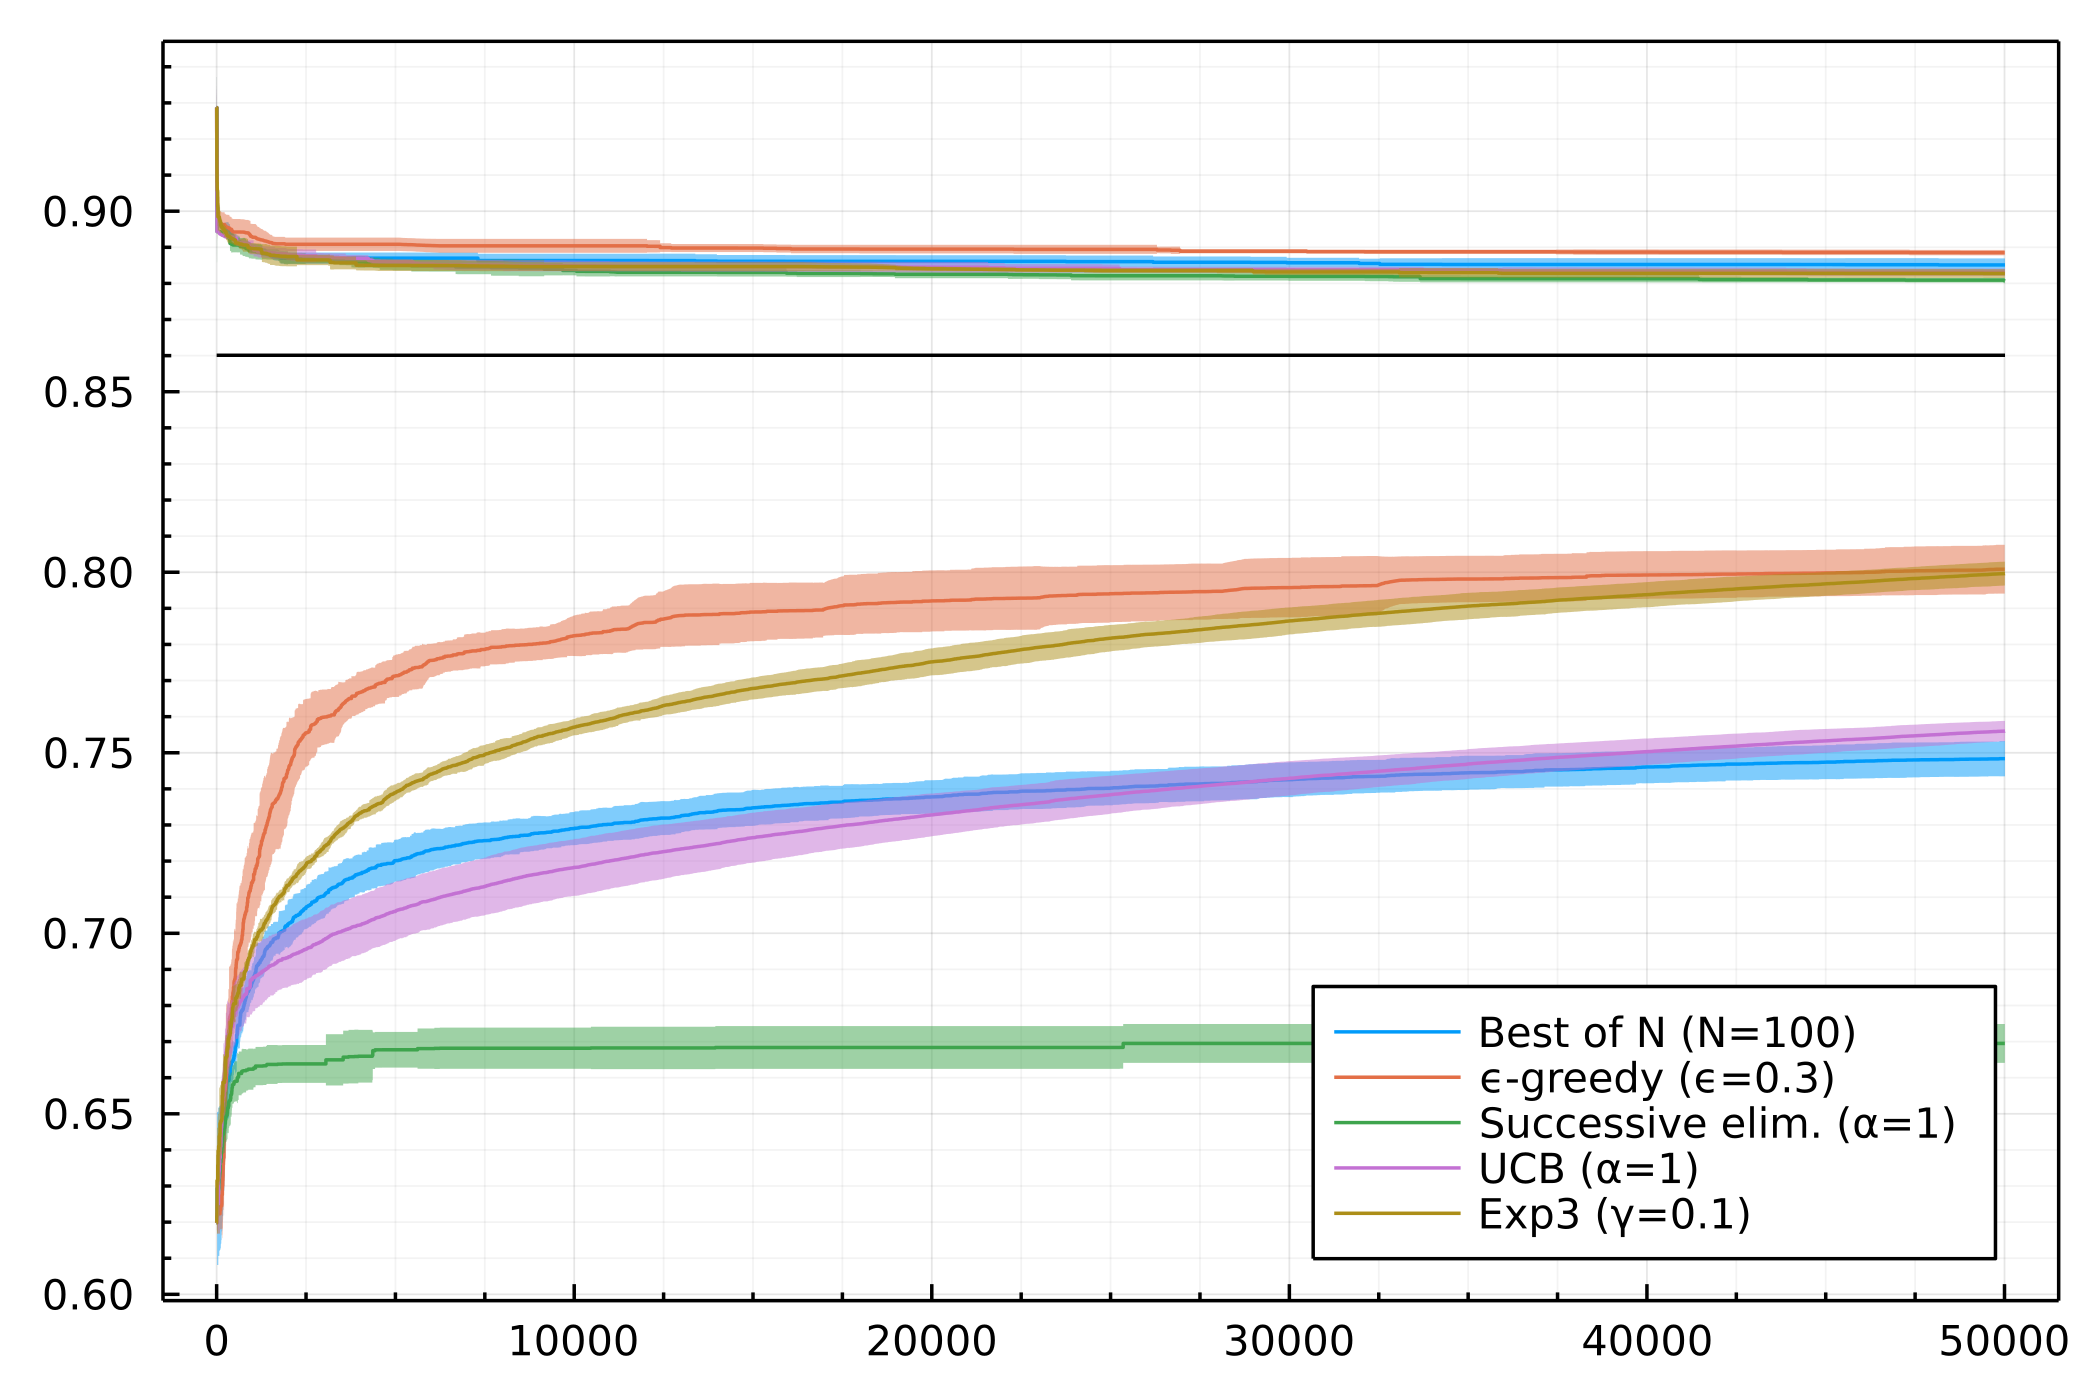
\includegraphics[width=1\textwidth]{osposg/bulk/easier_discount_095.png}
        \caption{Value bounds for the modified setting \reffig{exp:osposg:type:fig:2}}
        \label{exp:osposg:bulk:fig:easier:bounds}
    \end{subfigure}
    \hfill
    \begin{subfigure}[t]{0.45\linewidth}
        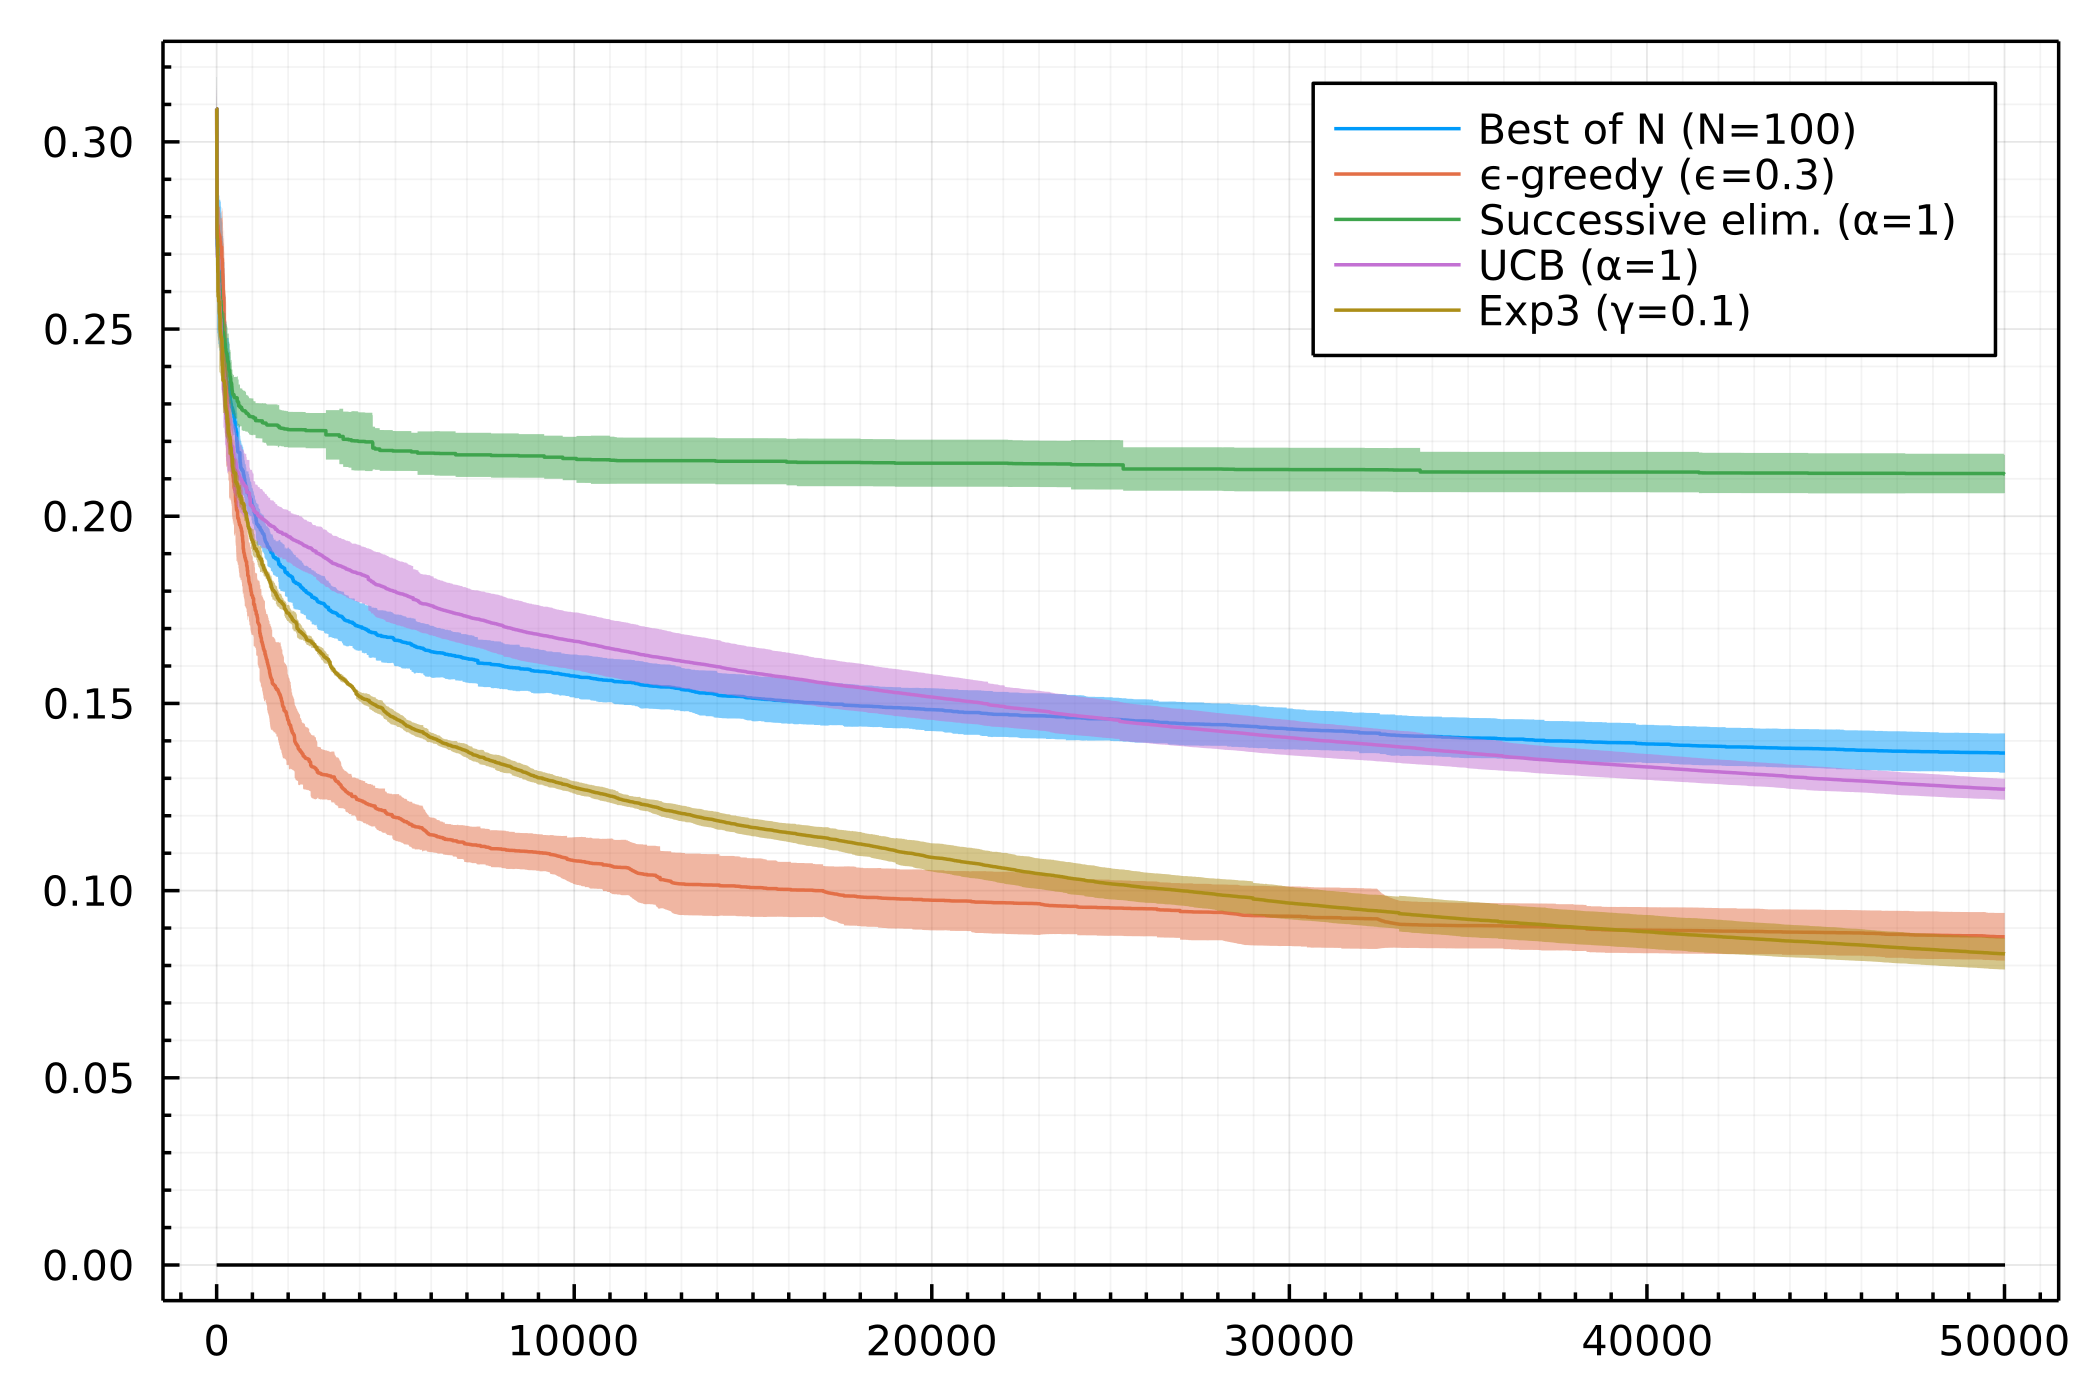
\includegraphics[width=1\textwidth]{osposg/bulk/gap_easier_discount_095.png}
        \caption{Gap between the bounds for the modified setting \reffig{exp:osposg:type:fig:2}}
        \label{exp:osposg:bulk:fig:easier:gap}
    \end{subfigure}
    \caption[Comparison of the multi-armed bandits on the \textbf{PEG} instance]{
        This figure depicts the convergence course of the multi-armed bandits with the best found parameters on the \textbf{PEG} instance with the use of discount factor $\gamma = 0.95$.
        The upper two graphs belong to the initial state in \reffig{exp:osposg:type:fig:1}, where the Pursuer is located in the upper left corner and initial belief $\binit$ is pure in the bottom right corner.
        The bottom two charts then belong to the initial state in \reffig{exp:osposg:type:fig:2}, with the Pursuer in the middle and the Evader with uniform probability in each corner.
        The left graphs show dependence of both lower and upper bounds on discrete time steps corresponding to bandit updates and the right graphs show decrease of the gap between bounds for the same time steps.
    }
    \label{exp:osposg:bulk:fig}
\end{figure}
The courses of convergence are very similar for all the runs, only the absolute values differ, thus it suffices to discuss a single case.

The Successive elimination bandit algorithm performs by far the worst on the lower bound.
The upper bound is by a tiny margin better, but it does not suffice to make it a suitable algorithm as the lower bound slowly converges to a completely different value.

Surprisingly, the Best of N algorithm is for many bandit updates better than the UCB.
On the easier initial setting in the lower half of the \reffig{exp:osposg:bulk:fig} the UCB at last overcomes the Best of N, so this can be expected even for the harder problem in later iterations after the predefined horizon.
This can be caused by the setting of the parameter $N$.
Until all actions are tried, the search is conducted as uniform sampling over the actions and thus provides enough exploration power to improve quickly, but after the best action is fixed, no exploration is conducted by the bandit.
The only exploration at that moment is the randomized selection of $\alpha$-vectors, but evidently it is not enough and the more explorative UCB continues slowly improving.
Note, however, that this holds only for the selected $\alpha$ for UCB, as for higher values it does not converge to the true value at all.

The best two algorithms are $\epsilon$-greedy and Exp3 which both get closer to the real value, for the easier example in the bottom half of \reffig{exp:osposg:bulk:fig} the gap between bounds gets even under 0.1.
Even though, the $\epsilon$-greedy with $\epsilon = 0.3$ improves very quickly at the beginning, in later iterations the improvements slows down as are more often chosen random actions which do not move the values in the correct direction on average.
Again, an adaptive annealing approach could help overcome this issue.
In contrast, the Exp3 improves more steadily and does not slow down as much and based on the trends in the chart, it would continue converging while the $\epsilon$-greedy would slow down more.

In the upper bound there are not very large differences between the individual bandit algorithms, but that is caused by the presolve procedure which gets the initial approximation really close to the real value.
However, the bottom graphs in \reffig{exp:osposg:bulk:fig} suggest that the situation is different, because it seems like the $\epsilon$-greedy is the worst, while Exp3 and Successive elimination are closest to the optimal value.

To obtain the best performance, the suggestion would be to use the Exp3 algorithm and fine-tune its $\gamma$ parameter more thoroughly, or use a combination of different bandits for the upper resp. lower bound.

\section{Summary}
In this chapter, we compared the bandit algorithms on different instances of games \textit{Tag} and \textit{Chase}.
Generally, it can be said, that neither Best of N, Successive elimination nor their observable variants are usable in the context of games as they discard some actions during the learning without possible correction and thus can prevent themselves from finding the optima.

From the other bandit algorithms the best option is the observable UCB multi-armed bandit in combination with the $\sqrtt$ averaging step function as they almost always converge quickly and without fluctuations in value.
The Exp3 bandit is also very good but sometimes struggles with speed and frequent oscillation around the optimal value with the $\sqrtt$ step.
The observable $\epsilon$-greedy usually performs well but cannot compete with the two before.
Unsurprisingly, the non-observable variants of $\epsilon$-greedy and UCB perform poorly as they seek to find a single best action.
These two algorithms converge slowly and often to some suboptimal value.

It turns out, that the average play employed in the observable bandits is a powerful factor in quality of the solution.
Also, the speed increasing $\sqrtt$ step is convenient and works really well for the average play UCB.
The other algorithms are then caused to oscillate because of it.
Perhaps, some function which decreases more rapidly than $\frac{1}{\sqrt{t}}$ but slower than $\frac{1}{t}$ could be proposed and lead to better results without fluctuations.

Then, we focused on the OS-POSG model and the proposed B-HSVI algorithm, which uses multi-armed bandits as well.
This time, however, only the non-observable variants as they fit the OS-POSG model more.
The comparisons of the bandit algorithms were conducted on a game of \textit{Pursuit-Evasion} of size $3 \times 3$.

The experimental evaluation showed surprising results as the UCB algorithm whose observable complement mostly dominated in the context of observable SGs, now does not perform well except for a very specific choices of parameters.
On the other hand, the $\epsilon$-greedy algorithm outperformed its expectations as it did not converge as good in stochastic games.
The Exp3 algorithm was consistently good and fulfilled its promises gained by performing well before, except for the fluctuations caused mainly by the alternative step function $\sqrtt$.

To conclude this chapter, we evaluated the bandit algorithms on two large domains of problems and compared their performance on specific instances.
Some of them exceeded their anticipated results, some did not fulfil them.
If a single bandit algorithms needed to be selected for each domain, it would be the \textit{Observable UCB} bandit for stochastic games as it is able to converge to real values even for states with randomized strategies and the \textit{Exp3} for One sided partially observable stochastic games as it performed consistently good for both upper and lower bound and showed more potential even after the fixed discrete horizon in the number of bandit updates.

\end{document}
